\documentclass[12pt,a4paper,twoside,openany]{book}
\usepackage[utf8]{vietnam}
\def\i{\item}
\setcounter{chapter}{4}
%\setcounter{section}{28}
\usepackage{picture} %Công cụ tạo header dọc trang (quay header)
\usepackage{cite}
\usepackage{ifthen}
\usepackage{amsmath,amssymb,pb-diagram}
\usepackage{comment}
\usepackage{multirow}
\usepackage{indentfirst}
\usepackage[width=19.20cm, height=26.90cm, left=2.20cm, right=2.20cm, top=2.20cm, bottom=2.20cm]{geometry}
\setlength{\parindent}{0cm}% Thụt lề
\setlength{\parskip}{2.2pt} % khoảng cách giữa 2 đoạn văn bản
\linespread{1.2}  % dãn dòng
\usepackage[svgnames,table]{xcolor}
\usepackage[all]{xy}
\usepackage{bbding}
\usepackage{stmaryrd}
\usepackage{mathptmx}
\usepackage{float}
\usepackage{multicol}
\usepackage{tabularx,booktabs}
\newcolumntype{Y}{>{\centering\arraybackslash}X}
\def\tieudeduoi{Nắm chắc kiến thức và kĩ năng toán 6}
\def\i{\item}
%%%===================Qrcode==============================%%%
%\usepackage{tikz}
%\usepackage{qrcode}				%Qrcode
%\def\maQR#1#2{
%	\tikz\path
%	node[above,draw=black,line width=2pt,rounded corners=1mm]{\qrcode[height=1in]{#2}}
%	node[below,rounded corners=1mm]{\href{#2}{#1}}
%	;
%}
%%%===========================================================%%%
%%%%%%%%%%%%%%%%%%%%%%%%%%%%%%%%%%%%%%%%%%
\usepackage[shortlabels]{enumitem}
\setenumerate{itemsep=1pt,topsep=1pt}
\setlist[enumerate,1]{itemsep=0pt,topsep=0pt,label=\protect\circled{\arabic*}}
\setlist[enumerate,2]{itemsep=0pt,topsep=0pt,label=\protect\circledqd{\small\alph*},wide=0.5cm,
leftmargin=0.5cm}
\setlist[enumerate,3]{itemsep=0pt,topsep=0pt,label=\protect\circledh{\small\roman*},wide=1cm,leftmargin=1cm}
\setlist[itemize,1]{itemsep=0pt,topsep=0pt,label=\protect{\small\starletdot}}
\setlist[itemize,2]{itemsep=0pt,topsep=0pt,label=\protect{\small\rhombusdot},wide=0.35cm,
leftmargin=0.35cm}
\setlist[itemize,3]{itemsep=0pt,topsep=0pt,label=\protect{\small\faAngellist},wide=0.5cm,leftmargin=.5cm}
%%%%%%%%%%%%%%%%%%%%%%%%%%%%%%%%%%%%%%%%%%%%%%%%
\usepackage{fancyhdr}
\renewcommand{\headrulewidth}{0pt}
%\renewcommand\sectionmark[1]{%
%	\markright{Bài \thesection.\ #1}}
%\renewcommand{\chaptermark}[1]{\markboth{Chuyên đề \thechapter.\ #1}{}}
%%%%%%%%%%%%%%%%%%%%%%%%%%%%%%%%%%%%%%%%%
\usepackage{graphicx}
\usepackage[labelsep=period]{caption}
\usepackage{subcaption}
%%%%%%%%%%%%%%%%%%%%%%%%%%%%%%%%%%%%%%%%%%%

%%%%%%%%%%%%%%%%%%%%%%%%%%%%%%%%%%%%%%%%%%
\newcommand\vt[1]{\overrightarrow{#1}}
\newcommand\sm[1]{{\displaystyle\sum\limits_{i=1}^{#1}}}
\newcommand\sk[1]{{\displaystyle\sum_{i=0}^{#1}}}
%%%%%%%%%%%%%%%%%%%%%%%%%%%%%%%%%%%%%%%%%
%Theorem
\usepackage{pgf,tikz,pgfplots}
\usetikzlibrary{arrows}
\usetikzlibrary[patterns]
\usetikzlibrary{shapes.geometric}
%%%%%%%%%%%%%%%%%%%%%%%%%%%%%%%%%%%%%%%%%%%%%
%%  Điều chỉnh chữ trong tiêu đề
\setcounter{secnumdepth}{5}
\numberwithin{equation}{section}
\numberwithin{figure}{section}
\renewcommand{\thepart}{\Roman{part}.}
\renewcommand{\thechapter}{\arabic{chapter}}
\renewcommand{\thesection}{{\usefont{T5}{uag}{db}{sc}vấn đề \arabic{section}.}}
\renewcommand{\thesubsection}{\Alph{subsection}.}
\renewcommand{\thesubsubsection}{\arabic{subsubsection}.} \renewcommand{\theequation}{\arabic{chapter}.\arabic{section}.\arabic{equation}}
\renewcommand{\thefigure}{\arabic{chapter}.\arabic{section}.\arabic{figure}}
%%%%%%%%%%%%%%%%%%%%%%%%%%%%%%%%%%%%%%%%%%%%%%%%%%%%
%%%%%%%%%%%%%%%%%%%%%%%%%%%%%%%%%%%%%%%%%%%%%%%%%%%%%%%%
%\usepackage[answerdelayed]{exercise}
%\renewcommand{\QuestionNB}{(\alph{Question})}
%\renewcommand{\AnswerHeader}{\vspace*{-16pt}}
%\setlength{\ExerciseSkipBefore}{0.1\baselineskip}
%\setlength{\ExerciseSkipAfter}{0pt}
%\setlength{\QuestionBefore}{1pt}
%\font\nsieu=vnr10 at 1pt
%%%%%%%%%%%%%%%%%%%%%%%%%%%%%%%%%
\def\R{\mathbb{R}}
\def\N{\mathbb{N}}
%%%%%%%%%%%%%%%%%%%%%%%%%%%%%%%%%%%%%%%%%%%%%%%%
\usepackage{wrapfig}
\usepackage{yhmath}%\wideparen
%%%%%%%%%%%%%%%%%%%%%%%%%%%%%%%%%%%%%%%%%%%%%%%%%%%%%%%%%
%\usepackage{contour} %Lặp lại từ, dùng làm đậm small cap
\usepackage{multido}
%%%%%%%%%%%%%%%%%%%%%%%%%%%%%%%%%%%%%%%%%%
%%%%%%%%%%%%%%%%%%%%%%%%%%%%%%%%%%%%%%%%%%%%
%%%Môi trường liệt kê
\usepackage{oplotsymbl} % Biểu tượng
\usepackage{fontawesome} %Biểu tượng
\newcommand\circled[1]{\tikz[baseline=(char.base)]{
     \node[shape=circle,minimum size =15pt,
     inner sep=1.25pt] (char) 
            {\fontfamily{qhv}\bfseries\small\selectfont#1};}}
\newcommand\circledqd[1]{\tikz[baseline=(char.base)]{\node[shape=circle,fill=cyan!10,draw,inner sep=1pt,
outer sep=0pt,minimum size =15pt,font=\fontsize{12}{12}\selectfont] (char){#1};}}
\newcommand\circledh[1]{\tikz[baseline=(char.base)]{\node[shape=circle,draw,minimum size =15pt, 
inner sep=1.25pt,font=\fontsize{12}{12}\selectfont] (char){#1};}}
\newcommand\diamondnumh[1]{\tikz[baseline=(char.base)]
	\node[draw,double,diamond, text width=9pt,align=center,inner sep=1pt,font=\fontsize{12}{12}\selectfont\bfseries] (char){#1};}
\usetikzlibrary{intersections,shadings,calc,angles,quotes}
\usepackage{tkz-euclide}
\usepackage{tkz-tab}
%\definecolor{xanhnhat}{RGB}{224,255,255}
%%%%%%%%%%%%%%%================================%%%%%%%%%%%%%
%%%Dóng khung
\newcommand\khungct[1]
{\noindent
\begin{tikzpicture}%
	\tikzstyle{khung} = [rectangle, inner sep=8pt,double]%
	\node [khung] {%
		$
		\; #1.\;
		$
	};%
	\end{tikzpicture}}
\newcommand\khung[1]
{\noindent\begin{tikzpicture}%
	\tikzstyle{khung} = [rectangle, inner sep=6pt,thick]%
	\node [khung]{%
		$
		\; #1\;
		$
	};%
	\end{tikzpicture}}
%%%%====================================================%%%%
%%%===================Hệ hoặc, hệ và===================%%%
\newcommand{\hoac}[1]{
\left[\begin{aligned}#1\end{aligned}\right. }
\newcommand{\heva}[1]{
\left\{\begin{aligned}#1\end{aligned}\right.}
\usepackage{longtable}
%%%================Viết tắt lệnh=========================%%%%
\usepackage{pgfornament}
\def\cao{1.7}
\pagestyle{fancy}
\fancyhf{}
\fancyhead[CO]{%Header trang lẻ
\begin{tikzpicture}[overlay, remember picture]%
\begin{scope}
	\clip (current page.north west)  rectangle ($(current page.north east)+(0,-1.5*\cao)$);
	%Đường trên trên
     \draw[line width=0.8pt] ($ (current page.north west)-(1cm,0.9*\cao)$) -- +(1.132*\textwidth,0) coordinate(A)--([turn]-60:0.36*\cao)--+(0.56*\cao,0)--([turn]60:0.36*\cao) coordinate(B)--+(0.3*\textwidth,0);
%     Đường kẽ dưới
     \draw[line width=0.8pt] ($ (current page.north west)-(1cm,0.94*\cao)$) -- +(1.138*\textwidth,0)  
     --([turn]-60:0.26*\cao)--+(0.524*\cao,0)--([turn]60:0.26*\cao) --+(0.3*\textwidth,0);
	%Node chương
    \node[anchor=north west, inner sep=0mm, shift={(2cm,-0.55*\cao)},text width=0.9*\textwidth] at ([xshift=0.2cm]current page.north west) {
    {\it\leftmark}}; 
  	%Node trang
   \node[draw,regular polygon,regular polygon sides=6,inner sep=2pt, outer sep =5mm,minimum size=0.95*\cao cm,line width=1pt] at 
   ([yshift=9pt,xshift=-0.25pt]$0.5*(A)+0.5*(B)$) {\fontfamily{qhv}\selectfont\bfseries\thepage};	
\end{scope}
\end{tikzpicture}
} 

\fancyhead[CE]{%Header trang chẵn
\begin{tikzpicture}[overlay, remember picture]%
\begin{scope}
	\clip (current page.north west)  rectangle ($(current page.north east)+(0,-1.5*\cao)$);
	%Đường trên trên
	\draw[line width=0.8pt] ($ (current page.north east)-(-1cm,0.9*\cao)$) -- +(-1.132*\textwidth,0) coordinate(A) %
	--([turn]60:0.36*\cao)--+(-0.56*\cao,0)--([turn]-60:0.36*\cao) coordinate(B)--+(-0.3*\textwidth,0);
	%Đường kẽ dưới
	\draw[line width=0.8pt] ($ (current page.north east)+(1cm,-0.94*\cao)$) -- +(-1.138*\textwidth,0)--([turn]60:0.26*\cao)--+(-0.524*\cao,0)--([turn]-60:0.26*\cao) --+(-0.3*\textwidth,0);
	%Node chương
	\node[anchor=north east, inner sep=0mm, shift={(-2cm,-0.55*\cao)},text width=0.925\linewidth,align=right] at ([xshift=-0.1cm]current page.north east){\itshape\rightmark}; 
	%Node trang
	\node[draw,regular polygon,regular polygon sides=6,inner sep=2pt , outer sep =5mm,minimum size=0.95*\cao cm,line width=1pt] at 
	([yshift=9pt, xshift = 0.26pt]$0.5*(A)+0.5*(B)$) {\fontfamily{qhv}\selectfont\bfseries\thepage};	
\end{scope}
\end{tikzpicture}
}




\fancyfoot[CO]{%Footer trang lẻ
    \begin{tikzpicture}[overlay, remember picture]%
    \clip (current page.south west) rectangle ($(current page.south east)+(0,1.5*\cao)$);  
    %Đường trên
    \draw[line width=0.8pt] ($(current page.south west)+(0,0.55*\cao)$) -- +(2.65*\cao,0) -- ([turn]60:0.4*\cao)--+(1.3*\textwidth,0); 
    %Đường kẽ dưới
	\draw[line width=0.8pt] ($(current page.south west)+(0,0.25*\cao)$) -- +(2.42*\cao,0) -- ([turn]60:0.7*\cao)--+(1.3*\textwidth,0); 
     %Chữ footer 
	\node[anchor=south, minimum size=.5in, yshift=0.01cm ] at ([xshift=1cm]current page.south)
    {\it\tieudeduoi};
\end{tikzpicture}
}

\fancyfoot[CE]{%Footer trang chẵn
    \begin{tikzpicture}[overlay, remember picture]%
    \clip (current page.south west) rectangle ($(current page.south east)+(0,1.5*\cao)$);  
    %Đường kẻ trên
    \draw[line width=0.8pt] ($(current page.south east)+(0,0.55*\cao)$) -- +(-2.65*\cao,0) -- ([turn]-60:0.4*\cao)-- +(-1.3*\textwidth,0); 
    %Đường kẻ dưới
	\draw[line width=0.8pt] ($(current page.south east)+(0,0.25*\cao)$) -- +(-2.42*\cao,0) -- ([turn]-60:0.7*\cao)-- +(-1.3*\textwidth,0);  
    %Chữ footer 
    \node[anchor=south, minimum size=.5in, yshift=0.01cm ] at ([xshift=-1cm]current page.south)
    {\it\tieudeduoi};
\end{tikzpicture}
}

\usepackage[most,many]{tcolorbox} 
\tcbuselibrary{skins}
\usetikzlibrary{shadings}
\usetikzlibrary{shadows}
\usepackage{varwidth}
\usepackage{collect}
\definecollection{btcol}
\definecollection{vdcol}
\definecollection{excol}
%%%==========Lệnh lời giải==========%%%
\newcommand{\loigiai}[1]{}
%%%==========Môi trường chèn hình==========%%%
\newdimen\widthimmini
\newdimen\heightimmini
\newdimen\textimagewidth
\newbox\imbox
\newcommand{\immini}[3][-12pt]{
		\setbox\imbox=\vbox{\hbox{#3}}
		\widthimmini=\wd\imbox
		\heightimmini=\ht\imbox	
		\textimagewidth=\dimexpr\linewidth - 1.075\widthimmini\relax
\par\vspace*{\dimexpr#1\relax}\noindent{\ignorespaces\begin{minipage}[t]{\textimagewidth}
	\vspace*{0pt}\ignorespaces
	\begingroup
	#2
	\endgroup
	\end{minipage}~
	\begin{minipage}[t]{\widthimmini}
	\vspace*{-1pt}
\begin{center}
	\begingroup
		#3
	\endgroup
\end{center}
\end{minipage}}}

\DeclareSymbolFont{yhlargesymbols}{OMX}{yhex}{m}{n}
\DeclareMathAccent{\wideparen}{\mathord}{yhlargesymbols}{"F3}

\newlength\boxwidth
\newbool{btracnghiem}
\newbool{blbaitap}
\newbool{blvd}

\definecolor{nennam}{RGB}{238,238,238}
\definecolor{maukhung}{RGB}{255,246,143}
\def\boxhead{
    \settowidth\boxwidth{Ví dụ 99}
\begin{tcolorbox}[breakable,top=0.5cm,bottom=-0.1cm,enhanced,before skip=10pt,after skip=5mm,
    boxsep=2mm,attach boxed title to top left={xshift=5mm,yshift=-\tcboxedtitleheight},boxrule=0.75pt,
    colback=nennam!25,rounded corners=southeast,arc=3.5pt,arc is curved,drop fuzzy shadow,left=5pt,right=5pt,
	title={\makebox[1.15\boxwidth][c]{}},
	 boxed title style={interior empty,frame code={
	 	       \filldraw[fill=nennam!80,line width=0.7pt] ([xshift=5mm]frame.north east) coordinate (B) arc (180:0:1mm)
	 	         ([xshift=3mm]frame.north west) coordinate (A)   arc(0:180:1mm);
	 	        \filldraw[fill=nennam!25,line width=0.65pt]
	 	        	 	       ([shift={(-.115,.1)}]A)--([shift={(.1cm,.1)}]B)[rounded corners=1mm]--([shift={(0,0)}]B)--([shift={(-0.1cm,-15pt)}]B)
	 	        	 	       --([shift={(0.1cm,-15pt)}]A)
	 	        	 	       --([shift={(0,0)}]A)[rounded corners=1mm]--([shift={(-.115,.1)}]A);
	 	       \path ([shift={(0pt,-6pt)}]A)--([shift={(0,-6pt)}]B) 
	 	      node[midway]{\refstepcounter{vd}\bfseries\fontfamily{pag}\selectfont Ví dụ \thevd};  
	  }}	 	      
      ]}
 \newcommand{\boxend}{\end{tcolorbox}}


%%%%==========Môi trường ví dụ==========%%%
\newcounter{vd}[section]

\newcommand{\ghichuvd}{}
\BeforeBeginEnvironment{vd}{\global\setbool{blvd}{true}
	\global\setbool{blbaitap}{false}\global\setbool{bltracnghiem}{false}}
\newenvironment{vd}[1][]{\Pluudapan%điều khiển lưu đáp
	\boxhead \ifthenelse{\equal{#1}{}}{\gdef\ghichuvd{}}{\gdef\ghichuvd{\par\hfill{(\textit{#1})}}}}
{\ghichuvd\boxend}
\newcommand{\khongindapanvd}{\renewcommand{\boxend}{\end{tcolorbox}}
\renewcommand{\loigiai}[1]{}
}

\newcommand{\indapanvd}{
	\renewcommand{\loigiai}[1]{
\renewcommand{\boxend}{\end{tcolorbox}\vspace*{-15pt}\begin{center}
	{\fontfamily{qag}\bfseries\selectfont Lời giải}\\[-19pt]
	\end{center}\vspace*{-15pt}
	\hspace*{-0.2cm}
	##1}}}


%%%=================moi truong bai tap=================%%%
\newcommand{\namebt}{Bài tập }
\def\boxheadbt{\begin{tcolorbox}[enhanced,breakable,
	before skip=2mm,after skip=9pt,
    left=1mm,right=1mm,top=2mm,bottom=1mm,
%	colback=gray!10,
	boxrule=0pt,
	arc=3mm,rounded corners,
	colbacklower=white, frame hidden]}
\newcommand{\boxendbt}{\end{tcolorbox}}
\makeatletter
\newcounter{bt}
\AtBeginEnvironment{bt}{\global\setbool{blvd}{false}
	\global\setbool{blbaitap}{true}\global\setbool{bltracnghiem}{false}}
\newenvironment{bt}[1][]{
	\refstepcounter{bt}\Pluudapan%điều khiển lưu đáp 
	\ifthenelse{\equal{#1}{}}{\boxheadbt{{\bfseries \namebt \thechapter.\thebt.  }}}
	{\boxheadbt{{\bfseries\namebt \thechapter.\thebt \ (#1). }}}}
	{\boxendbt} 
\makeatother
\newcommand{\khongindapanbaitap}{\renewcommand{\boxendbt}{\end{tcolorbox}}
	\renewcommand{\loigiai}[1]{
			\begin{Answer}
			\begingroup
			##1
			\endgroup
			\end{Answer}
	}
}
\newcommand{\indapanbaitap}{
	\renewcommand{\loigiai}[1]{
	\renewcommand{\boxendbt}{\end{tcolorbox}
	{\bfseries\selectfont\noindent \hdg}\\[0pt]
	##1
	}
	}
}

%%%============Môi trường đóng khung============%%%
\RequirePackage[framemethod=default]{mdframed}

%\newmdenv[skipabove=7pt,
%skipbelow=7pt,
%rightline=false,
%leftline=true,
%topline=false,
%bottomline=false,
%backgroundcolor=black!5,
%innerleftmargin=5pt,
%innerrightmargin=5pt,
%innertopmargin=5pt,
%leftmargin=0cm,
%rightmargin=0cm,
%linewidth=3pt,
%innerbottommargin=5pt]{cBox}
%
%\newmdenv[skipabove=7pt,
%skipbelow=7pt,
%rightline=false,
%leftline=true,
%topline=false,
%bottomline=false,
%linecolor=orange,
%backgroundcolor=nennam,
%innerleftmargin=5pt,
%innerrightmargin=5pt,
%innertopmargin=5pt,
%leftmargin=0cm,
%rightmargin=0cm,
%linewidth=3pt,
%]{bBox}

%\newmdenv[skipabove=7pt,
%skipbelow=7pt,
%rightline=false,
%leftline=true,
%topline=false,
%bottomline=true,
%backgroundcolor=nennam,
%innerleftmargin=5pt,
%innerrightmargin=5pt,
%innertopmargin=5pt,
%leftmargin=0cm,
%rightmargin=0cm,
%linewidth=2pt,
%]{dnBox}
%%%=============Moi truong dn==================%%%
%\newcounter{sodn}[section]
%\newenvironment{dn}{\begin{dnBox}\refstepcounter{sodn}
%{\fontfamily{qag}\selectfontĐịnh nghĩa \arabic{chapter}.\arabic{section}.\thesodn}.\;
%}
%{\end{dnBox}}

%%%%==============Moi truong dang====================%%%
%\definecolor{xanh}{HTML}{04AA6D}
%\definecolor{xanhdatroi}{HTML}{2196F3}
%\definecolor{cam}{HTML}{ff9800}
%\definecolor{do}{HTML}{f44336}
%
%\newcounter{sodang}[section]
%\makeatletter
%\def\calcLength(#1,#2)#3{%
%\pgfpointdiff{\pgfpointanchor{#1}{center}}%
%             {\pgfpointanchor{#2}{center}}%
%\pgf@xa=\pgf@x%
%\pgf@ya=\pgf@y%
%\FPeval\@temp@a{\pgfmath@tonumber{\pgf@xa}}%
%\FPeval\@temp@b{\pgfmath@tonumber{\pgf@ya}}%
%\FPeval\@temp@sum{(\@temp@a*\@temp@a+\@temp@b*\@temp@b)}%
%\FProot{\FPMathLen}{\@temp@sum}{2}%
%\FPround\FPMathLen\FPMathLen5\relax
%\global\expandafter\edef\csname #3\endcsname{\FPMathLen}
%}
%\makeatother
%
%\newmdenv[skipabove=7pt,
%skipbelow=7pt,
%rightline=false,
%leftline=true,
%topline=false,
%bottomline=false,
%linecolor=xanhdatroi,
%backgroundcolor=nennam,
%innerleftmargin=5pt,
%innerrightmargin=5pt,
%innertopmargin=5pt,
%leftmargin=0cm,
%rightmargin=0cm,
%linewidth=2pt,
%]{dangBox}
%
%\newenvironment{dang}[1][]{\begin{dangBox}\refstepcounter{sodang}\setcounter{vd}{0}
%\begin{tikzpicture}[remember picture,overlay]
%\path (-6pt,7pt) node[fill=xanhdatroi,inner sep=6pt,text width=0.975\linewidth,anchor=north west] (AT)
%	{{\bfseries\fontfamily{pag}\selectfont\color{white}Dạng~\arabic{section}.\thesodang. #1}};
%\path (AT.north east) coordinate (A)
%		(AT.south east) coordinate (B)
%		($ (A)!0.5!(B) $) coordinate (C);
%\calcLength(A,C){mylen}
%\draw[xanhdatroi,ultra thick,fill=white] ([xshift=0.5*\mylen]C) 
%coordinate (TC) let  \p1 = ($ (C) - (A) $),  \n1 = {veclen(\x1,\y1)} 
% in circle (1.25*\n1);
% \path (TC) let  \p1 = ($ ([xshift=-12pt]C) - (A) $),  \n1 = {veclen(\x1,\y1)} 
%  in  node{\includegraphics[width=\n1]{Khaibao/pencil}};
%\end{tikzpicture}
%
%\par\bigskip\noindent
%}
%{\end{dangBox}}

%%%================Moi truong phuong phap===================%%%
%\newmdenv[skipabove=7pt,
%skipbelow=7pt,
%rightline=false,
%leftline=true,
%topline=false,
%bottomline=false,
%linecolor=cam,
%backgroundcolor=nennam,
%innerleftmargin=5pt,
%innerrightmargin=5pt,
%innertopmargin=5pt,
%leftmargin=0cm,
%rightmargin=0cm,
%linewidth=2pt,
%]{ppBox}
%
%\newenvironment{pp}[1][]{\begin{ppBox}
%\begin{tikzpicture}[remember picture,overlay]
%\path (-6pt,7pt) node[fill=cam,inner sep=6pt,text width=0.975\linewidth,anchor=north west] (AT)
%	{{\bfseries\fontfamily{pag}\selectfont\color{white}Phương pháp #1}};
%\path (AT.north east) coordinate (A)
%		(AT.south east) coordinate (B)
%		($ (A)!0.5!(B) $) coordinate (C);
%\calcLength(A,C){mylen}
%\draw[cam,ultra thick,fill=white] ([xshift=0.5*\mylen]C) 
%coordinate (TC) let  \p1 = ($ (C) - (A) $),  \n1 = {veclen(\x1,\y1)} 
% in circle (1.25*\n1);
% \path (TC) let  \p1 = ($ ([xshift=-12pt]C) - (A) $),  \n1 = {veclen(\x1,\y1)} 
%  in  node{
\includegraphics[width=\n1]{Khaibao/Key}};
%\end{tikzpicture}
%
%\par\bigskip\noindent
%}
%{\end{ppBox}}



%%%================Moi truong phan tich===================%%%
%\newenvironment{pt}
%{\begin{TCBox}{\fontfamily{qag}
%			\bfseries\selectfont Phân tích:\\ }}
%	{\end{TCBox}}

%%%=============Moi truong hệ quả==================%%%
%\newcounter{sohq}[section]
%\newenvironment{hq}{\begin{cBox}\refstepcounter{sohq}
%{\fontfamily{qag}\selectfontHệ quả \arabic{chapter}.\arabic{section}.\thesohq}.\;
%}{\end{cBox}}

%%%%=============Moi truong bổ đề==================%%%
%\newcounter{sobd}[section]
%\newenvironment{bd}{\begin{cBox}\refstepcounter{sobd}
%		{\fontfamily{qag}\selectfont Bổ đề 
%			\arabic{section}.\thesobd}.\;
%	}{\end{cBox}}
%
%%%%=============Moi truong tính chất==================%%%
%\newmdenv[skipabove=5pt,
%skipbelow=5pt,
%rightline=false,
%leftline=true,
%topline=false,
%bottomline=false,
%backgroundcolor=nennam,
%innerleftmargin=5pt,
%innerrightmargin=5pt,
%innertopmargin=5pt,
%leftmargin=0cm,
%rightmargin=0cm,
%linewidth=3pt,
%innerbottommargin=5pt
%]{TCBox}
%\newcounter{sotc}[section]
%\newenvironment{tc}
%{\begin{TCBox}{\fontfamily{qag}\refstepcounter{sotc}
%\bfseries\selectfont Tính chất \arabic{section}.\thesotc.}}
%{\end{TCBox}}
%%%%=============Moi truong chứng minh==================%%%
%\newenvironment{proof}{\noindent{ \bf\textit{ Chứng minh}}\\}{}
%%%%=============Moi truong nx==================%%%
%\newenvironment{nx}
%{\begin{TCBox}{\fontfamily{qag}
%\bfseries\selectfont Nhận xét: }}
%{\end{TCBox}}
%%%%=============Moi truong lời giải==================%%%
%\newenvironment{dapan}{\noindent{ \bf{ \hdg}}\\}{}
%%%%=============Moi truong đề thi==================%%%
%\newenvironment{dethi}{\refstepcounter{bt}\noindent{ \bf{ Câu \thebt.  }}}{}
%%%%=============Moi truong dl==================%%%
%\newmdenv[skipabove=7pt,
%skipbelow=7pt,
%rightline=false,
%leftline=true,
%topline=false,
%bottomline=false,
%backgroundcolor=nennam,
%innerleftmargin=5pt,
%innerrightmargin=5pt,
%innertopmargin=5pt,
%leftmargin=0cm,
%rightmargin=0cm,
%linewidth=3pt,
%innerbottommargin=5pt
%]{DLBox}
%
%\newcounter{sodl}[section]
%\newenvironment{dl}
%{\begin{DLBox}{\fontfamily{qag}\refstepcounter{sodl}
%\bfseries\selectfont Định lý \arabic{section}.\thesodl.}}
%{\end{DLBox}}

%%%=============Moi truong chú ý==================%%%
\newmdenv[skipabove=7pt,
skipbelow=7pt,
rightline=false,
leftline=true,
topline=false,
bottomline=false,
%backgroundcolor=black!5!white,
innerleftmargin=5pt,
innerrightmargin=5pt,
innertopmargin=0pt,
leftmargin=0cm,
rightmargin=0cm,
linewidth=3pt,
innerbottommargin=0pt
]{NoteBox}

%\newenvironment{cy}
%{\begin{NoteBox}{\fontfamily{qag}\refstepcounter{sodl}
%\bfseries\selectfont Chú ý}. }
%{\end{NoteBox}}

\newenvironment{ly}
{\begin{NoteBox}{\fontfamily{qag}
%			\refstepcounter{sodl}
\bfseries\selectfont Lưu ý}.}
{\end{NoteBox}}

%%%======================Box cho tiểu mục lục=================
%\newmdenv[skipabove=7pt,
%skipbelow=7pt,
%rightline=false,
%leftline=false,
%topline=true,
%bottomline=true,
%backgroundcolor=nennam,
%innerleftmargin=1pt,
%innerrightmargin=1pt,
%innertopmargin=5pt,
%leftmargin=0cm,
%rightmargin=0cm,
%linewidth=2pt,
%]{bhBox}
% 
%\newmdenv[skipabove=7pt,
%skipbelow=7pt,
%rightline=false,
%leftline=true,
%topline=false,
%bottomline=false,
%backgroundcolor=nennam,
%innerleftmargin=5pt,
%innerrightmargin=5pt,
%innertopmargin=5pt,
%leftmargin=12cm,
%rightmargin=12cm,
%linewidth=3pt,
%]{bmBox}
%%%======================================================%%%
%%%====================Phần trắc nghiệm======================%%%
\usepackage{mathrsfs}  
\usepackage{ifthen}
\usepackage{etoolbox}
\usepackage{intcalc}%Tính mod
\usepackage{forloop}
%\usepackage{catchfile}%đưa file vào văn bản ngay lập tức
\newcounter{ex}[section]%số câu hỏi
\newcounter{dapan}[ex] %Số thứ tự a, b, c, d để đưa vào đáp án
\newcounter{numTrue}[ex]%Số thứ tự đáp án của câu
\newcommand{\dotEX}{.}%dấu kết thúc mỗi phương án
\newbool{bltracnghiem}%Kiểm tra có phải trắc nghiệm không
%%%==========khoanh đáp án===========%%%
%\newcommand\excircled[1]{\tikz[baseline=(char.base)]{\node[shape=circle,draw,line width=0.65pt,
%inner sep=1pt,fill=cyan!15,
%minimum size =13pt,font=\fontfamily{pag}\fontsize{9.5pt}{10pt}\selectfont] (char){#1};}}
%\newcommand\excircledda[1]{\tikz[baseline=(char.base)]{\node[shape=circle,draw,line width=0.65pt,
%inner sep=1pt,fill=orange!15,
%minimum size =13pt,font=\fontfamily{pag}\fontsize{10pt}{10pt}\bfseries\selectfont] (char){\color{orange}#1};}}
%\newcommand\excircledxanh[1]{\tikz[baseline=(char.base)]{\node[shape=circle,draw,line width=0.65pt,
%inner sep=1pt,
%minimum size =13pt,font=\fontfamily{pag}\fontsize{10pt}{10pt}\bfseries\selectfont] (char){#1};}}
%%%==========môi trường ex==========%%%
%%\AtBeginEnvironment{ex}{\vspace*{-1.25\parskip}}
%\newcommand{\exhead}[1][]{\par\noindent\refstepcounter{ex}
%%Thông tin đầu câu trắc nghiệm
%%{\fontfamily{pag}\fontsize{11pt}{13pt}\selectfont\bfseries Câu \arabic{chapter}.\arabic{section}.\arabic{ex}.}\
%{\fontfamily{pag}\fontsize{11pt}{12pt}\selectfont\bfseries Câu \arabic{ex}.\ignorespaces
%\ifthenelse{\equal{#1}{}}{}{{(\textit{#1})}}}
%\global\setbool{bltracnghiem}{true}
%}%khai báo của môi trường ex
%\newcommand{\exend}{%Kết thúc môi trường trắc nghiệm
%\renewcommand{\loigiai}[1]{\begin{Answer}
%	{\noindent{\small\usefont{T5}{HLButlong}{m}{n} \dauloigiaitracnghiem}
%	##1\par\noindent
%	Chọn đáp án \excircledda{\Alph{numTrue}}
%  	}
% \end{Answer}
%}
%\renewcommand{\exend}{\shipoutAnswer}}%Kết thúc môi trường trắc nghiệm
%%\newcommand{\indapan}{\shipoutAnswer}
%\newcommand{\dapansaucauhoi}{
%\renewcommand{\loigiai}[1]{\begin{Answer}
%	{\noindent{\small\usefont{T5}{HLButlong}{m}{n} \dauloigiaitracnghiem}
%	##1\par\noindent
%	Chọn đáp án \excircledda{\Alph{numTrue}}
%  	}
% \end{Answer}
%}
%\renewcommand{\exend}{\shipoutAnswer}
%\renewcommand{\exbend}{\medskip\shipoutAnswer}}
%\newcommand{\khongindapansaucauhoi}{
%\renewcommand{\loigiai}[1]{\begin{Answer}
%	{\noindent{\small\usefont{T5}{HLButlong}{m}{n} \dauloigiaitracnghiem}
%	##1\par\noindent
%	Chọn đáp án \excircledda{\Alph{numTrue}}
%  	}
% \end{Answer}
%}

%\def\tabex{20pt}%Thụt đầu dòng của trắc nghiệm tính bằng pt
%\def\tieudeboxvd{Câu} %tiêu đề trong nhãn của ô
%
%\renewcommand{\exend}{}}
%\newcommand{\khongluuloigiai}{\renewcommand{\loigiai}{}}
%%%%================Môi trường ex================%%%
%\AtBeginEnvironment{ex}{\global\setbool{blvd}{false}
%	\global\setbool{blbaitap}{false}\global\setbool{bltracnghiem}{true}}
%\newenvironment{ex}[1][]{\Pluudapan%điều khiển lưu đáp 
%\refstepcounter{ex}%%%===phần tiêu đầu câu
%\par\noindent{\selectfont\bfseries  Câu \arabic{ex}\ignorespaces}\ifthenelse{\equal{#1}{}}{\,}{\,{ (\textit{#1}).}}\unskip%%%===phần ghi chú câu
%\unskip}{\exend}
%%%%%%%%Tự động chọn \motcot, \haicot, \boncot
%     	\newlength\widthcha
%        \newlength\widthchb
%        \newlength\widthchc
%        \newlength\widthchd
%        \newlength\widthch
%        \newlength\tabmaxwidth
%        \newlength\fourthtabwidth
%        \newlength\halftabwidth
%        \newlength\fifthtabwidth
%        \newlength\thirdtabwidth
%\setlength\fourthtabwidth{\dimexpr0.225\linewidth-0.25\tabex-30pt\relax}
%\setlength\halftabwidth{\dimexpr 0.475\linewidth-0.5\tabex-20pt\relax}
%\newcommand{\choice}[4]{
%\settowidth\widthch{#1}
%\settowidth\widthchb{#2}
%\ifdim\widthch<\widthchb\relax\setlength{\widthch}{\widthchb}\fi%
%\settowidth\widthchc{#3}%
%\ifdim\widthch<\widthchc\relax\setlength{\widthch}{\widthchc}\fi%
%\settowidth\widthchd{#4}%
%\ifdim\widthch<\widthchd\relax\setlength{\widthch}{\widthchd}\fi%
%\ifdim\widthch<\fourthtabwidth
%     \boncot{#1}{#2}{#3}{#4}
%      \else\ifdim\widthch<\halftabwidth
%          \haicot{#1}{#2}{#3}{#4}
%        \else
%          \motcot{#1}{#2}{#3}{#4}
%      \fi
%\fi}

%\newcommand{\boncot}[4]{
%	\setlength{\topsep}{0pt}%
%   \setlength{\partopsep}{0pt}%
%  \begin{tabbing}
%  \hspace*{\tabex}\=
%  \hspace*{\dimexpr0.25\linewidth-0.25\tabex\relax}
%  \=\hspace*{\dimexpr0.25\linewidth-0.25\tabex\relax}
%  \=\hspace*{\dimexpr0.25\linewidth-0.25\tabex\relax}
%  \=\kill
%  \phantom{a}\>
%  \refstepcounter{dapan}\excircled{A} #1\dotEX
%  \>
%  \refstepcounter{dapan}\excircled{B} #2\dotEX
%  \>
% \refstepcounter{dapan}\excircled{C} #3\dotEX
%  \>
% \refstepcounter{dapan}\excircled{D} #4\dotEX\vspace*{-1.25\parskip}
%\end{tabbing}
%%\end{center}
%}
   
%\newcommand{\haicot}[4]{
% \setlength{\topsep}{0pt}%
% \setlength{\partopsep}{0pt}%
% \begin{tabbing}
% \hspace*{\tabex}\= \hspace*{\dimexpr0.5\linewidth-0.5\tabex+6pt\relax}\=\kill
%  \phantom{a}\>\refstepcounter{dapan}\excircled{A} #1\dotEX\>
%   \refstepcounter{dapan}\excircled{B} #2\dotEX\\ 
%  \phantom{a}\>\refstepcounter{dapan}\excircled{C} #3\dotEX\>
%    \refstepcounter{dapan}\excircled{D} #4\dotEX\vspace*{-1.25\parskip}
%\end{tabbing}
% }
%\newcommand{\motcot}[4]{
% \par\noindent
%\hspace*{\tabex}\refstepcounter{dapan}\excircled{A} #1\dotEX\\
%\hspace*{\tabex}\refstepcounter{dapan}\excircled{B} #2\dotEX\\ 
%\hspace*{\tabex}\refstepcounter{dapan}\excircled{C} #3\dotEX\\
%\hspace*{\tabex}\refstepcounter{dapan}\excircled{D} #4\dotEX
%}

%%%===========in đáp án==============%%%
%\def\alist{}
%\def\True{\ignorespaces\setcounter{numTrue}{\thedapan}{\ifnum\value{numTrue}=1 \listgadd{\alist}{A}\fi
%	\ifnum\value{numTrue}=2 \listgadd{\alist}{B}\fi
%	\ifnum\value{numTrue}=3 \listgadd{\alist}{C}\fi
%	\ifnum\value{numTrue}=4 \listgadd{\alist}{D}\fi}} 
%\renewcommand{\loigiai}[1]{\begin{Answer}
%\ifbool{bltracnghiem}
%	{\noindent{\small\usefont{T5}{HLButlong}{m}{n} \dauloigiaitracnghiem}
%	#1\par\noindent
%	Chọn đáp án \excircledda{\Alph{numTrue}}
%  	}
%  	{
%  	\begingroup
%  	#1
%  	\endgroup
%  	}
% \end{Answer}
%}
%%%===============In đáp án ra bảng=================%%%
%\newcounter{itemcount}
%\renewcommand*{\do}[1]
% {\refstepcounter{itemcount} #1}
%\dolistloop{\alist}

%%%=================môi trường task================%%%
%\usepackage{tasks}
%\settasks{
%  item-indent =\dimexpr \parindent+\parindent, 
%  before-skip = -1.5pt , % undo paragraph skip
%  after-skip =-2pt , % undo paragraph skip
%  after-item-skip =-2pt% undo paragraph skip
%}
%\AtBeginEnvironment{tasks}
%	{\mbox{}\vspace*{\dimexpr -\baselineskip+3mm}}
%	


%%=================Bảng đáp án=================%%
%\newcounter{itemcount}
%\def\bangdapan{
%\begin{center}
%	\begin{tcolorbox}[enhanced,hbox,
%			left=8mm,right=8mm,boxrule=0.4pt,
%			colback=white,
%			%drop fuzzy midday shadow=black!50!yellow,
%			drop lifted shadow=black!50!yellow,arc is angular,
%			before=\par\vspace*{-1mm},after=\par\bigskip]
%			{\bfseries\fontfamily{qag}\selectfont ĐÁP ÁN BÀI \arabic{section}} 
%		\end{tcolorbox}
%		\vspace*{-0.5cm}
%\end{center}
%
%\setcounter{itemcount}{0}
% \renewcommand*{\do}[1]{\refstepcounter{itemcount} 
% {\makebox[22pt][l]{\ifthenelse{\value{itemcount}<10}
% {\phantom{.}\theitemcount}{\theitemcount}.}~{\fontfamily{qag}\selectfont##1}}\ignorespaces
% \ifthenelse{\equal{\value{itemcount}}{\value{ex}}}{.}{,}
% \ifthenelse{\equal{\intcalcMod{\value{itemcount}}{10}}{0}}
%   {\newline}{}
% }
%\noindent\dolistloop{\alist}}


%%=================Bảng đáp án dạng hộp=================%%
%\newcounter{itemcounth}
%\def\bangdapanhop{
%\begin{center}
%	\begin{tcolorbox}[enhanced,hbox,
%			left=8mm,right=8mm,boxrule=0.4pt,
%			colback=white,
%			%drop fuzzy midday shadow=black!50!yellow,
%			drop lifted shadow=black!50!yellow,arc is angular,
%			before=\par\vspace*{-1mm},after=\par\bigskip]
%			{\bfseries\fontfamily{qag}\selectfont ĐÁP ÁN BÀI \arabic{section}} 
%		\end{tcolorbox}
%		\vspace*{-0.5cm}
%\end{center}

%\setlength{\fboxrule}{1pt}
%\setcounter{itemcounth}{0}
% \renewcommand*{\do}[1]{\refstepcounter{itemcounth} 
% \fcolorbox{black}{cyan!10}{\makebox[1cm][c]{
% {\theitemcounth.}\ignorespaces{\fontfamily{qag}\bfseries\selectfont\color{violet}##1 }}}
% \ifthenelse{\equal{\intcalcMod{\value{itemcounth}}{10}}{0}}
% {\par\noindent\ignorespaces}{}
% }
%\noindent\dolistloop{\alist}}
%
%\begin{center}
%{\fontfamily{qag}\selectfont Đáp án dạng danh sách, dùng đưa vào các ứng dụng chấm điểm}
%\end{center}
%\renewcommand*{\do}[1]
% {\refstepcounter{itemcount} 
% \ifthenelse{\equal{\value{itemcount}}{\value{ex}}}
% {#1.}
% {#1,}
% }
% \setcounter{itemcount}{0}
%\noindent\dolistloop{\alist}

%%%=====================khung trac nghiem=====================%%%
%\newtcolorbox{vdbox}[2][]{
%	enhanced,
%	before skip=2mm,after skip=2mm,
%	top=2pt,bottom=5pt,left=6pt,right=3pt,
%	colback=nencl,colbacktitle=nencl,
%	colframe=khungcl,
%	boxrule=0.2mm, %width=0.95\linewidth,
%	attach boxed title to top left={xshift=1cm,yshift*=1mm-\tcboxedtitleheight},
%	varwidth boxed title*=-3cm,
%	boxed title style={
%		frame code={
%			\draw[color=khungcl,line width=0.2mm,fill=black!30]
%			([yshift=-1mm,xshift=-1mm]frame.north west)
%			arc[start angle=0,end angle=180,radius=1mm]
%			([yshift=-1mm,xshift=1mm]frame.north east)
%			arc[start angle=180,end angle=0,radius=1mm];
%			\draw[color=khungcl,fill=nencl,line width=0.2mm]
%			([xshift=-2mm]frame.north west) -- ([xshift=2mm]frame.north east)
%			[rounded corners=1mm]--
%			([xshift=1mm,yshift=-1mm]frame.north east) -- (frame.south east) --
%			(frame.south west) -- ([xshift=-1mm,yshift=-1mm]frame.north west)
%			[sharp corners]-- cycle;
%		},
%		interior engine=empty,
%	},
%	fonttitle=\fontfamily{pag}\fontsize{11pt}{11pt}\bfseries\selectfont,
%	title={#2},#1
%}
%%%=====================Het khung trac nghiem=====================%%%
%%%==============Moi truong vdex===============%%%
%\newcommand{\exbend}{\end{vdbox}}
%\AtBeginEnvironment{exb}{\global\setbool{bltracnghiem}{true}\global\setbool{blvd}{false}
%\global\setbool{blbaitap}{false}}
%\newenvironment{exb}[1][]{\refstepcounter{ex}\Pluudapan%điều khiển lưu đáp 
%\ifthenelse{\equal{#1}{}}{\begin{vdbox}{\tieudeboxvd\ \theex}}
%{\begin{vdbox}{\tieudeboxvd\ \theex\ {\mdseries({\small\textit{#1}})}}}
%}
%{\exbend}
%%%==============Hết moi truong vdex===============%%%

 
%%%============Dòng kẻ 22/7=============%%%
%\newcommand{\exbdongke}{}
%\newcommand{\sodongke}[1][5]{
%\ifnum #1>0
%	\renewcommand{\exbdongke}{
%		\begin{center}
%		{\fontfamily{qag}\selectfont\bfseries Bài Làm}\vspace*{-\baselineskip}
%		\end{center}
%		\foreach \k in {1,...,#1}
%			{\par\vspace*{2pt}\noindent\makebox[\linewidth]{\dotfill}}
%	}
%\else
%	\renewcommand{\exbdongke}{}
%\fi
%}
%%%============Het dòng kẻ 22/7=============%%%
%%%============Tạo dòng kẻ 22/7=============%%%
%\newcommand{\taodongke}[1][5]{
%	\sodongke[#1]	
%	\global\setbool{blluudapan}{true}
%}
%\newcommand{\vohieuhoadongke}{\renewcommand{\taodongke}[1][]{}}
%%%============Het tạo dòng kẻ 22/7=============%%%



%\newcommand{\hdg}{Hướng dẫn giải}
%%%%============Lenh hien thi dap an=============%%%
%\newcommand{\hienthidapan}{\global\setbool{blluudapan}{false}
%	\renewcommand{\exbdongke}{}
%	\renewcommand{\loigiai}[1]{\ifbool{blvd}{
%		\renewcommand{\boxend}{\end{tcolorbox}
%			\vspace*{-\baselineskip}
%			\begin{center}
%			{\bfseries\selectfont Lời giải} 
%			\end{center}
%%			\vspace*{-0.8\baselineskip}
%			\begingroup
%			\noindent##1
%			\endgroup}
%		 }{\ifbool{blbaitap}{
%		 		\renewcommand{\boxendbt}{\end{tcolorbox}
%		 			\vspace*{-\baselineskip}
%		 			\begin{center}
%		 			{\it\bfseries\selectfont\noindent \hdg\\
%		 			} 
%		 			\end{center}
%		 			\vspace*{-0.8\baselineskip}
%		 			\begingroup
%		 			\noindent##1
%		 			\endgroup}
%		 	 }{\ifbool{bltracnghiem}{
%		 	 		 		\renewcommand{\exend}{\par\noindent{\small\usefont{T5}{HLButlong}{m}{n} \dauloigiaitracnghiem}
%		 	 		 				##1\par\noindent
%		 	 		 				Chọn đáp án \excircledda{\Alph{numTrue}}
%		 	 		 			}
%		 	 		 	  \renewcommand{\exbend}{\end{vdbox}\par\noindent{\small\usefont{T5}{HLButlong}{m}{n} \dauloigiaitracnghiem}
%		 	 		 	  		 	 	##1\par\noindent
%		 	 		 	  		 	 	Chọn đáp án \excircledda{\Alph{numTrue}}
%		 	 		 	  		 	}
%		 	 }{}}		 
%		 }
%	}
%}
%%%============Hết lenh hien thi dap an=============%%%

%%%============Lenh luu dap an=============%%%
\newbool{blluudapan}
\newcommand{\luudapan}{\sodongke[0]
	\global\setbool{blluudapan}{true}
}
\makeatletter
\newcommand{\loigiai@aux}[2]{a}
\newcommand{\Pluudapan}{ 
%%%==================xử lý câu đầu tiên
\ifbool{blluudapan}{
\ifbool{blvd}{ %truong hop vi 
		\renewcommand{\loigiai}[1]{%
		  \@bsphack\expandafter\loigiai@aux\expandafter{\expanded{\thevd}}{##1}\@esphack
		}
		\renewcommand{\loigiai@aux}[2]{%
		  \begin{collect}{vdcol}{\par\noindent{\fontfamily{qag}\bfseries
		  	\small\selectfont  VD ##1}.\ignorespaces}{}{}{} 
			##2%
		  \end{collect}
		}
	\renewcommand{\boxend}{\end{tcolorbox}\exbdongke}
	}{\ifbool{blbaitap}{ % truong hop bai tap
			\renewcommand{\loigiai}[1]{%
			  \@bsphack\expandafter\loigiai@aux\expandafter{\expanded{\thebt }}{##1}\@esphack
			}
			\renewcommand{\loigiai@aux}[2]{%
			  \begin{collect}{btcol}{\par\noindent{\fontfamily{qag}\bfseries
			  	\small\selectfont  BT ##1}.\ignorespaces}{}{}{} 
				##2%
			  \end{collect}
			}
		\renewcommand{\boxendbt}{\end{tcolorbox}\vspace*{3pt}\exbdongke}
		}{\ifbool{bltracnghiem}{ % truong hop trac nghiem
					\renewcommand{\loigiai}[1]{%
					  \@bsphack\expandafter\loigiai@aux\expandafter{\expanded{\theex.\Alph{numTrue}}}{##1}\@esphack
					}
					\renewcommand{\loigiai@aux}[2]{%
					  \begin{collect}{excol}{\par\noindent{\fontfamily{qag}\bfseries
					  	\small\selectfont  TN ##1}.\ignorespaces}{}{}{} 
						##2
					  \end{collect}
					}
				\renewcommand{\exend}{\exbdongke} 
			    \renewcommand{\exbend}{\end{vdbox}\exbdongke} 
				}{}
		}
	}
}{}%ket thuc dieu kien luu an
}
\makeatother

%%%============Hết lenh luu dap an=============%%%

%%%============Lenh in dap an vi du=============%%%
%\newcommand{\dapanvidu}{
%\begin{center}
%%{\usefont{T5}{HLButlong}{m}{n} ĐÁP ÁN VÍ DỤ}
%{\bfseries\fontfamily{ugq}\selectfont ĐÁP ÁN VÍ DỤ}
%\end{center}
%\vspace*{-\baselineskip}
%\includecollection{vdcol}}
%%%============Hết lenh in dap an vi du=============%%%

%%%============Lenh in dap an bai tap=============%%%
%\newcommand{\dapanbaitap}{
%\begin{center}
%%{\usefont{T5}{HLButlong}{m}{n} ĐÁP ÁN VÍ DỤ}
%{\bfseries\fontfamily{ugq}\selectfont ĐÁP ÁN BÀI TẬP}
%\end{center}
%\vspace*{-\baselineskip}
%\includecollection{btcol}}
%%%============Hết lenh in dap an bai tap=============%%%

%%%============Lenh in dap an bai tap=============%%%
%\newcommand{\dapantracnghiem}{
%\begin{center}
%%{\usefont{T5}{HLButlong}{m}{n} ĐÁP ÁN VÍ DỤ}
%{\bfseries\fontfamily{ugq}\selectfont ĐÁP ÁN TRẮC NGHIỆM}
%\end{center}
%\vspace*{-\baselineskip}
%\includecollection{excol}}
%%%============Hết lenh in dap an bai tap=============%%%

%%%============Dat noi dung cau hoi=============%%%
%\newtcolorbox{cauhoi}[1][]{enhanced,breakable,
%	before skip=1mm,after skip=1mm,
%	boxrule=0pt,left=11mm,right=0mm,top=3mm,bottom=1mm,
%	arc=0mm,colback=white,fontupper={\fontfamily{pag}\selectfont\fontsize{13pt}{13pt}},
%	underlay={%
%		\path  node at ([shift={(5mm,2pt)}]interior.west){
\includegraphics[height=25pt]{Khaibao/Logo.pdf}};
%	},
%	#1}	
%%%============Het dat noi dung cau hoi=============%%%


%%%%%%%%%%%%%%%%%%%%%%%%%%%%%%%%%%%%%%%%%%%%%%%%%%%%%%%
%\newcommand{\dauloigiaitracnghiem}{Hướng dẫn:} %%%chi tiết hơn thì dùng lệnh ở dưới
%%%\newcommand{\dauloigiaitracnghiem}{Hướng dẫn giải Câu \arabic{ex}.}
%%%\hienthidapan
%%%\luudapan
%%%\dongke
%\newcommand{\dapso}[1]{
%	\luudapan %điều chỉnh in hay không in đáp án khi có đáp số
%	\renewcommand{\boxendbt}{\end{tcolorbox}
%	\phantom{a}\hfill
%	\begingroup
%	{\usefont{T5}{HLButlong}{m}{n}Đáp số:} #1
%	\endgroup
%}
%\renewcommand{\boxend}{\end{tcolorbox}
%\phantom{a}\hfill
%\begingroup
%{\usefont{T5}{HLButlong}{m}{n}Đáp số:} #1
%\endgroup
%}
%}


%%%==========Môi trường chia cột================%%%
%\setlength\multicolsep{0pt}
%\newlist{listEXt}{enumerate}{2}
%\setlist[listEXt]{label=\protect\circled{\alph*},topsep=0pt,itemsep=0pt}
%\newenvironment{listEX}[1][2]
%{\begin{multicols}{#1}\begin{enumerate}[label=\protect\circled{\alph*}]}
%{\end{enumerate}\end{multicols}}
%%%==========Hết môi trường chia cột================%%%

\DeclareSymbolFont{AMSb}{U}{msb}{m}{n}
\makeatletter
\DeclareSymbolFontAlphabet{\math@bb}{AMSb}
\AtBeginDocument{\protected\def\mathbb{\math@bb}} 
\g@addto@macro\normalsize{
\setlength{\abovedisplayskip}{4pt}%
\setlength{\belowdisplayskip}{2pt}%
\setlength{\abovedisplayshortskip}{4pt}%
\setlength{\belowdisplayshortskip}{1pt}%
}
\makeatother

%%%=== KÍ HIỆU CUNG ===
\usetikzlibrary{tikzmark}
%\newcommand{\arc}[1]{%
%\tikzmarknode{a}{#1}
%\begin{tikzpicture}[overlay,remember picture]
%\draw ([yshift=1pt]a.north west) to[bend left=20] ([yshift=1pt]a.north east);
%\end{tikzpicture}%
%}
%%=== KÍ HIỆU ĐỒNG DẠNG ===
%\renewcommand{\backsim}{\ 
%\mathord{\raisebox{0.035\baselineskip}
%{\rotatebox{90}{\fontfamily{qag}\selectfont S}}}\
%} 
%%=== KÍ HIỆU SONG SONG ===
\usepackage{indentfirst}
%\DeclareSymbolFont{symbolsC}{U}{txsyc}{m}{n}
%\DeclareMathSymbol{\varparallel}{\mathrel}{symbolsC}{9}
%\renewcommand{\varparallel}{\mathbin{\! \raisebox{0.025\baselineskip}/ \mkern-2mu \raisebox{0.025\baselineskip}/ \!}}
%\renewcommand{\parallel}{\mathbin{\! \raisebox{0.025\baselineskip}/ \mkern-2mu \raisebox{0.025\baselineskip}/ \!}}


%%%%============Khai báo lệnh viết tắt TIKZ=============%%%
%
%\def\tructam(#1,#2,#3)(#4){
%	%Trực tâm tam giác
%	\path
%	($(#1)!(#3)!(#2)$) coordinate (zzzz1)
%	($(#1)!(#2)!(#3)$) coordinate (zzzz2)
%	(intersection of #3--zzzz1 and #2--zzzz2) coordinate (#4)
%	;
%}
%\def\trongtam(#1,#2,#3)(#4){
%	%Trọng tâm tam giác
%	\path
%	($(#1)!0.5!(#2)$) coordinate (zzzz1)
%	($(#1)!0.5!(#3)$) coordinate (zzzz2)
%	(intersection of #3--zzzz1 and #2--zzzz2) coordinate (#4)
%	;
%}
%\def\noitiep(#1,#2,#3)(#4){
%	%Tầm đường tròn nội tiếp
%	\path
%	($(#1)!1mm!(#2)$) coordinate (a1)
%	($(#1)!1mm!(#3)$) coordinate (a2)
%	($(a1)!0.5!(a2)$) coordinate (at)
%	($(#2)!1mm!(#1)$) coordinate (b1)
%	($(#2)!1mm!(#3)$) coordinate (b2)
%	($(b1)!0.5!(b2)$) coordinate (bt)
%	(intersection of #1--at and #2--bt) coordinate (#4)
%	;
%}
%\def\ngoaitiep(#1,#2,#3)(#4){
%	%Tầm đường tròn ngoại tiếp
%	\path
%	($(#1)!0.5!(#2)$) coordinate (A1)
%	($(A1)!1mm!90:(#2)$) coordinate (d1)
%	($(#1)!0.5!(#3)$) coordinate (A2)
%	($(A2)!1mm!90:(#1)$) coordinate (d2)
%	(intersection of A1--d1 and A2--d2) coordinate (#4)
%	;
%}
%\def\dtron(#1,#2){
%	% Đường tròn tâm A bán kính AB
%	\path[name path =#1#2] (#1) let\p1=($(#1)-(#2)$) in circle ({veclen(\x1,\y1)});
%	\draw (#1) let\p1=($(#1)-(#2)$) in circle ({veclen(\x1,\y1)});
%}
%%Chân đường phân giác
%\def\chanpg(#1,#2,#3)(#4){
%	\path let
%	\p1=($(#2)-(#1)$),\p2=($(#2)-(#3)$),
%	\n1={veclen(\x1,\y1)},\n2={veclen(\x2,\y2)}
%	in ($(#1)!scalar((\n1)/(\n1+\n2))!(#3)$) coordinate(#4);
%}
%%Tâm đường tròn bàng tiếp
%\def\bangtiep(#1,#2,#3)(#4){
%	\path
%	(#2)--(#1)--([turn]0:1) coordinate (p1t)
%	(#2)--(#3)--([turn]0:1) coordinate (p3t);
%	\chanpg(#3,#1,p1t)(p1tt)
%	\chanpg(#1,#3,p3t)(p3tt)
%	\coordinate (#4) at (intersection of #1--p1tt and #3--p3tt);
%}
%% Điểm đẳng giác của 4 qua tam giác 123 tên là 5
%\def\diemdanggiac(#1,#2,#3,#4)(#5){
%	\chanpg(#1,#2,#3)(pg2)
%	\chanpg(#1,#3,#2)(pg3)
%	\path 	($(#2)!(#4)!(pg2)$)	coordinate(pg22)
%	($(#4)!2!(pg22)$)	coordinate(dx2)
%	($(#3)!(#4)!(pg3)$)	coordinate(pg33)
%	($(#4)!2!(pg33)$)	coordinate(dx3)
%	(intersection of #2--dx2 and #3--dx3) coordinate (#5) 
%	;
%}
%\def\dxtruc(#1,#2,#3)(#4){
%	\path
%	($(#2)!(#1)!(#3)$)coordinate(hinhchieu1)
%	($(#1)!2!(hinhchieu1)$)coordinate(#4)
%	;
%}
%%% ------ Tọa độ điểm 
%\def\toado(#1){
%	\path 
%	(4,0) coordinate (xi)
%	(0,4) coordinate (yi)
%	(0,0) coordinate (O)
%	($(O)!(#1)!(xi)$) coordinate (x#1)
%	($(O)!(#1)!(yi)$) coordinate (y#1);
%	\draw[dashed] (x#1)--(#1)--(y#1);
%}
%%%============Kết thúc TIKZ=============%%%












\definecolor{doc}{RGB}{0,60,110}
\usepackage{titletoc}
\usepackage{pdfrender}
\usepackage{framed}
\contentsmargin{0cm}
\newcounter{sochuong} %điếm số chương
\setcounter{sochuong}{0}

\patchcmd{\tableofcontents}{\contentsname}{\sffamily\contentsname}{}{}
%%%=========================part================%%%
\makeatletter

\newif\ifnotstarredversion


\renewcommand*\l@part[2]{%
    \ifnum \c@tocdepth >-2\relax
    \addpenalty{-\@highpenalty}%
    \addvspace{10pt \@plus\p@}%
    \setlength\@tempdima{3em}%
    \begingroup
   \hypersetup{linkcolor=violet}
   \tikz[remember picture, overlay]{
	\draw[thick] (1,-7pt) coordinate (A) arc (270:90:14pt)
	--++(0.935*\linewidth,0) coordinate (B) arc (90:-90:14pt)--cycle;%
	\path (A)--(B) node[midway]
	{\bfseries\fontfamily{pag}\selectfont {\scshape Phần} #1 - Trang #2};
	}
    \par\smallskip
	\penalty\@highpenalty
	\setcounter{chapter}{0}
    \endgroup
    \fi
}

\def\@part[#1]#2{%
  \thispagestyle{fancy}
  \setcounter{chapter}{0}
  \startcontents[chapters]
  \refstepcounter{part}
  \addcontentsline{toc}{part}{\Roman{part}. #1}%
  \markboth{Phần \Roman{part}. #1}{Phần \Roman{part}. #1}%
  {\interlinepenalty \@M
    \begin{center}
    \begin{tikzpicture}[remember picture]
   		\path (0,0)  to [ornament=88] +(0.55\textwidth,0);
%		\path[blue] (-0.5,0) node[anchor=north west] {\pgfornament[width=1cm]{41}}
%		+(0.525\textwidth,0) node[anchor=north west] {\pgfornament[width=1cm,symmetry=v]{41}};
   		\path (0,-1) node[anchor=north west] (A){
   		\begin{minipage}{0.55\linewidth}
   		\begin{center}
%   		   			{\Huge\sffamily\bfseries Phần \Roman{part}.  \\[12pt]
%   		   		        \MakeUppercase{#2}}
				\textpdfrender{
					TextRenderingMode=FillStroke,
					LineWidth=0.4pt,
					FillColor=violet,
				}{\Huge\sffamily\bfseries Phần \Roman{part}}\\[15pt]
			    \textpdfrender{
			    					TextRenderingMode=FillStroke,
			    					LineWidth=0.4pt,
			    					FillColor=violet,
			    				}{\Huge\fontfamily{qag}\selectfont\bfseries \MakeUppercase{#2}}
   		\end{center}
   		\end{minipage}
   		};
   		\path ([yshift=-1cm]A.south west)  to [ornament=88] +(0.55\textwidth,0);
    \end{tikzpicture}
    \end{center}
      }%
      \@endpart
    }

\titlecontents{chapter}[0pc]
{\addvspace{20pt}%
\begin{tikzpicture}[remember picture, overlay]%
\draw[thick](-4,-7pt) -- (2.5,-7pt) arc (-90:90:13pt)--++(-6,0)--cycle;%
\node[anchor=east,align=right] at (2.75,5pt){{\fontfamily{pag}\bfseries\selectfont
 Chủ đề} {\large\fontfamily{phv}\selectfont\bfseries
 \thecontentslabel}};%
\end{tikzpicture}
\large\scshape\bfseries
\hypersetup{linkcolor=blue}
\hspace*{3.1cm}}%
{}
{}
{\;\titlerule\;\sc\bfseries Trang {\fontfamily{phv}\selectfont\ \thecontentspage}\begin{tikzpicture}[remember picture, overlay]
\draw (2pt,0) --+(3,0);
\end{tikzpicture}}%

\titlecontents{section}
  [1.5cm]
  {\vspace*{0.15\baselineskip}\sffamily\bfseries}{\makebox[1.4cm][l]{\thecontentslabel}}{}
  {\titlerule*[0.65pc]{.}\thecontentspage}

\titlecontents{subsection}
  [2.85cm]
  {\sffamily\vspace*{-0.15\baselineskip}}{\makebox[0.825cm][l]{\thecontentslabel}}{}  
{\titlerule*[1pc]{.}\thecontentspage}
\titlecontents{subsubsection}
  [3.5cm]
  {\sffamily\vspace*{-0.15\baselineskip}}{\makebox[0.825cm][l]{\thecontentslabel}}{}  
  {\titlerule*[1pc]{.}\thecontentspage}
%%%%%%%===================================================
%%%%%%Mục lục của chương
\titlecontents{uchapter}[0.1pt]
{}
{\thecontentslabel\; }
{}
{\titlerule*[0.65pc]{.}\thecontentspage}
[]

\titlecontents{usection}[0.1pt]
{}
{\thecontentslabel\; }
{}
{\titlerule*[0.65pc]{.}\thecontentspage}
[]

\titlecontents{usubsection}[0.75cm]
{\small} 
{\thecontentslabel\; }
{}
{{\titlerule}{\small\thecontentspage}}
[]
\makeatletter
\renewcommand{\tableofcontents}{%
\newpage
\markboth{Mục lục}{Mục lục}
%\renewcommand{\rightmark}{Mục lục}
\begin{center}
	\begin{tcolorbox}[enhanced,hbox,
			left=8mm,right=8mm,boxrule=0.4pt,
			colback=white,colframe=blue,
			%drop fuzzy midday shadow=black!50!yellow,
			drop lifted shadow=black!50!yellow,arc is angular,
			before=\par\vspace*{-1mm},after=\par\bigskip]
			{\bfseries\large\fontfamily{qag}\selectfont MỤC LỤC} 
		\end{tcolorbox}
\end{center}
\newcounter{somucluc}
\vskip-1.25cm
\@starttoc{toc}}
\makeatother
%%%%%%%%%%%%%%%%%%%%%%%%%%%%%%%%%%%%%%%%%%%%%%%%
%----------- Phần điều chỉnh hiển thị chapter - section - ....
%%%%%%%%%%%%%%%%%%%%%%%%%%%%%%%%%%%%%%%%%%%%%%%%%%%%
\usepackage[explicit]{titlesec}
\titlespacing*{\chapter}{0pt}{10pt}{0pt}%left,top,bottom
\titleformat{\chapter}[display]
{
   \thispagestyle{fancy}
   \startcontents[chapters]
}
{
\tikz[remember picture,overlay]
		{\draw[ultra thick,line join=bevel,opacity=0.75] (0,-0.2) coordinate(A)  --+(0.2*\textwidth,0) coordinate(B)
			 -- ([turn]55:0.11*\textwidth) coordinate(C)--+(0.758*\textwidth,0) coordinate(D);
		  \draw[line width=0.75pt,line join=bevel] (0,-0.135)--+(0.208*\textwidth,0) 
		  			 			 -- ([turn]55:0.11*\textwidth) --+(0.75*\textwidth,0) ;
		  %Node chữ chương
		  \node[anchor=south,inner sep=7pt] at   ([yshift=1pt]$0.5*(A)+0.5*(B)$) {
		   {\Large \it {\bfseries Chủ đề\ \thechapter}}};%\chaptertitlename
		 %Tên chương
	   	 \node[anchor=north,inner sep=3pt,text width=0.75*\textwidth,align=center] at ([yshift=-3pt]$0.5*(C)+0.5*(D)$) 
	   	 	{\fontfamily{qag}\LARGE\selectfont\bfseries\MakeUppercase{#1}};
		}	   	 
}{1em}{} 
%%%%%%%%%%%%%%%%%%%%%%%%%%%%%%%%%%%%%%%%%%%%%%%%%%%%%%%%%%
%%%%%%%%%%%%%%%%%%%%%%%%%%%%%%%%%%%%%%%%%%%%%%%%%%%%%%%%%%
\titleformat{\section}
{\normalfont\fontsize{12}{13}\bfseries\xdef\alist{}}
{\fontfamily{qhv}\selectfont\thesection}{.15em}
{\fontsize{12}{13}\fontfamily{qag}\selectfont
	{#1}}
[\color{black}]
%%---------------
\titleformat{\subsection}
{\normalfont\fontsize{10}{12}\bfseries\setcounter{vd}{0}}
{\fontsize{10}{12}{\bfseries\fontfamily{pag}\selectfont
\thesubsection}}{.5em}
{\fontsize{10}{12}\fontfamily{pag}\bfseries\selectfont#1}
[\color{black}]
%%-------------------
\titleformat{\subsubsection}
{\normalfont\fontsize{10}{12}\bfseries}
{\fontsize{10}{12}\bfseries\thesubsubsection}{.5em}
{\fontsize{10}{12}\selectfont#1}[]
%\titlespacing{\chapter}
%{0pc}{*0.5}{*6}[0pc]
%\titlespacing*{command}{left}{before-sep}{after-sep}[right-sep]
\titlespacing{\section}
{0pc}{*1.0}{*0.3}[0pc]
\titlespacing{\subsection}
{0pc}{*0.5}{*0.2}[0pc]
\titlespacing{\subsubsection}
{0pc}{*0.5}{*0.2}[0pc]
%%%%%%%%%%%%%%%%%%%%%%%%%%%%%%%%%%%%%%%%%%%%%
%Lien ket, phải đặt sau cùng
\usepackage[colorlinks=true,unicode]{hyperref}
\hypersetup{
	colorlinks=true,
	citecolor=black,
	linkcolor=black,
	%citecolor=green,
	%linkcolor=red,
	pagebackref=true,
	% linktocpage=true,
	bookmarksopen=true}
	
%%%=================In tiểu mục lục=================%%%
\newcommand{\tieumucluc}{
\noindent

\par\noindent
{\fontfamily{qag}\selectfont\bfseries\color{orange}Mục lục của Chủ đề \thechapter}
\vspace*{-\parskip}
\begin{center}
\begin{minipage}{0.8\linewidth}
\begin{bmBox}
	\hypersetup{linkcolor=violet}
	\printcontents[chapters]{u}{1}{\setcounter{tocdepth}{1}}
\end{bmBox}
\end{minipage}
\end{center}
\hypersetup{linkcolor=black}
}

%%%=================In tiểu mục lục hai=================%%%
%\newcommand{\tieumuclucH}{
%\noindent
%%\begin{minipage}{0.8\linewidth}
%\begin{bhBox}
%	\hypersetup{linkcolor=violet}
%	\printcontents[chapters]{l}{1}{\setcounter{tocdepth}{1}}
%\end{bhBox}
%%\end{minipage}
%\hypersetup{linkcolor=black}
%}

\makeatother
%%%%%%%%%%%%%%%%  Điều chỉnh Header
\renewcommand{\sectionmark}[1]
{\markright{\itshape\selectfont
		Vấn đề \arabic{section}.\ #1}}
\renewcommand{\chaptermark}[1]
{\markboth{Chủ đề \arabic{chapter}.\ #1}{}}




%\tcbuselibrary{raster}
%%Chia thành 2 cột
\newcommand{\haividu}[2]{
\begin{tcbraster}[%Chia làm 2 cột, 1 dòng
        raster columns=2,
        raster rows=1,
		raster equal height,
		size=small,colframe=cyan,colback=nencl,
		colbacktitle=nencl,
		raster left skip=0pt,
		raster right skip=0pt,
		left=1mm,right=1mm,
		top=3pt,bottom=3pt,
		arc is angular,
		arc=3pt,
%		title={\small\fontfamily{qag}\bfseries\selectfont\color{blue!70!black} Ví dụ \thetcbrasternum}
        ]
    %%%=============cột thứ nhất=============%%%
        \begin{tcolorbox}
        {\small\fontfamily{qag}\bfseries\selectfont Ví dụ \thetcbrasternum.} #1
        \end{tcolorbox}
     %%%===========cột thứ hai==============%%%
     \begin{tcolorbox}[enhanced,underlay={\begin{tcbclipinterior}
                \tikzset{daucham/.style={dash pattern=on .02mm off 2.mm, line cap=round}}
                \draw[daucham,line width=1pt,xstep=80,ystep=0.65,color=gray]
               ([xshift=5pt]interior.north west) grid ([xshift=-2pt]interior.south east);	
                \end{tcbclipinterior}}]
                    \begin{tcolorbox}[boxrule=0mm,
                         grow to left by=1mm,
                         grow to right by=1mm,
                         left=0pt,right=0pt,top=0pt,
                         sharp corners]
                   {\small\fontfamily{qag}\bfseries\selectfont Ví dụ \thetcbrasternum.}  #2
%                   {\vspace*{-12pt}\begin{center}
%                   {\bfseries\fontfamily{qag}\small\selectfont Bài làm}
%                   \end{center}}
            \end{tcolorbox}
      \end{tcolorbox}                 
\end{tcbraster}}
%%Chia ví dụ thành 4 cột
\newcommand{\bonvidu}[4]{
\begin{tcbraster}[%Chia làm 2 cột, 1 dòng
        raster columns=2,
        raster rows=2,
		raster equal height,
		size=small,colframe=cyan,colback=nencl,
		colbacktitle=nencl,
		raster left skip=0pt,
		raster right skip=0pt,
		left=1mm,right=1mm,
		top=3pt,bottom=3pt,
		arc is angular,
		arc=3pt,
%		title={\small\fontfamily{qag}\bfseries\selectfont\color{blue!70!black} Ví dụ \thetcbrasternum}
        ]
    %%%=============Ví dụ thứ nhất=============%%%
        \begin{tcolorbox}
        {\small\fontfamily{qag}\bfseries\selectfont Ví dụ \thetcbrasternum.} #1
        \end{tcolorbox}
     %%%===========Ví dụ thứ hai==============%%%
     \begin{tcolorbox}[enhanced,underlay={\begin{tcbclipinterior}
                \tikzset{daucham/.style={dash pattern=on .02mm off 2.mm, line cap=round}}
                \draw[daucham,line width=1pt,xstep=80,ystep=0.65,color=gray]
               ([xshift=5pt]interior.north west) grid ([xshift=-2pt]interior.south east);	
                \end{tcbclipinterior}}]
                    \begin{tcolorbox}[boxrule=0mm,
                         grow to left by=1mm,
                         grow to right by=1mm,
                         left=0pt,right=0pt,top=0pt,
                         sharp corners]
                   {\small\fontfamily{qag}\bfseries\selectfont Ví dụ \thetcbrasternum.}  #2
%                   {\vspace*{-15pt}\begin{center}
%                   {\bfseries\fontfamily{qag}\small\selectfont Bài làm}
%                   \end{center}}
            \end{tcolorbox}
      \end{tcolorbox}           
         %%%===========Ví dụ thứ ba==============%%%
         \begin{tcolorbox}[enhanced,underlay={\begin{tcbclipinterior}
                    \tikzset{daucham/.style={dash pattern=on .02mm off 2.mm, line cap=round}}
                    \draw[daucham,line width=1pt,xstep=80,ystep=0.65,color=gray]
                   ([xshift=5pt]interior.north west) grid ([xshift=-2pt]interior.south east);	
                    \end{tcbclipinterior}}]
                        \begin{tcolorbox}[boxrule=0mm,
                             grow to left by=1mm,
                             grow to right by=1mm,
                             left=0pt,right=0pt,top=0pt,
                             sharp corners]
                       {\small\fontfamily{qag}\bfseries\selectfont Ví dụ \thetcbrasternum.}  #3
%                       {\vspace*{-15pt}\begin{center}
%                       {\bfseries\fontfamily{qag}\small\selectfont Bài làm}
%                       \end{center}}
                \end{tcolorbox}
          \end{tcolorbox}            
         %%%===========Ví dụ thứ tư==============%%%
         \begin{tcolorbox}[enhanced,underlay={\begin{tcbclipinterior}
                    \tikzset{daucham/.style={dash pattern=on .02mm off 2.mm, line cap=round}}
                    \draw[daucham,line width=1pt,xstep=80,ystep=0.65,color=gray]
                   ([xshift=5pt]interior.north west) grid ([xshift=-2pt]interior.south east);	
                    \end{tcbclipinterior}}]
                        \begin{tcolorbox}[boxrule=0mm,
                             grow to left by=1mm,
                             grow to right by=1mm,
                             left=0pt,right=0pt,top=0pt,
                             sharp corners]
                       {\small\fontfamily{qag}\bfseries\selectfont Ví dụ \thetcbrasternum.}  #4
%                       {\vspace*{-15pt}\begin{center}
%                       {\bfseries\fontfamily{qag}\small\selectfont Bài làm}
%                       \end{center}}
                \end{tcolorbox}
          \end{tcolorbox}                 
\end{tcbraster}}

%%%==================Môi trường chấm bên phải================%%%
\newtcolorbox{rightdots}[1][5cm]{blanker,breakable,right=3mm+#1,left=0pt,top=0pt,bottom=0pt,
	code={\def\tabex{0pt}},
	underlay={
 	  \begin{scope}[line width=1.5pt,line cap=round]
			\tikzset{circle dotted/.style={dash pattern=on .02mm off 2.mm}}
			\draw[circle dotted,xstep=70,ystep=0.7,color=gray!70] (interior.north east) grid ([xshift=-#1]interior.south east);	
		\end{scope}}}
%\usepackage{paracol}
\tcbuselibrary{skins}
\usepackage{relsize}
\setlength{\columnsep}{4pt}
%%\setlength{\topsep}{0pt}
%%Chia thành 2 ô
\newcommand{\dauchamhaio}[3][7cm]{%
\begin{paracol}{2}
    %%%=============cột thứ nhất=============%%%
      \begin{tcolorbox}[breakable,enhanced,arc is angular,
              		arc=2pt,boxrule=0.35mm,
        			left=1mm,right=1mm,
        			top=3pt,bottom=3pt,
              		height=#1,
            		colback=white,
            		colframe=blue,
              	underlay={\begin{tcbclipinterior}
                 \tikzset{daucham/.style={dash pattern=on .9 mm off  0.6 mm, line cap=round}}
                 \draw[daucham,line width=0.5pt,xstep=80,ystep=0.85,color=gray!70]
                ([shift={(0,-5pt)}]interior.north west) grid (interior.south east);	
                 \end{tcbclipinterior}}]
                     \begin{tcolorbox}[boxrule=0mm,
                         colframe=white,
                          grow to left by=2mm,
                          grow to right by=2mm,
                          left=0pt,right=0pt,top=-3pt,
                          colback=white,
                          arc is angular,
                          arc=2pt]
                    {\fontfamily{qag}\bfseries\selectfont \relscale{0.9}{Luyện tập 1}.}  
                    #2
             \end{tcolorbox}
       \end{tcolorbox}       
     %%%===========cột thứ hai==============%%%
  \switchcolumn
     \begin{tcolorbox}[breakable,enhanced,arc is angular,
             		arc=2pt,boxrule=0.35mm,
       				left=1mm,right=1mm,
       				top=3pt,bottom=3pt,
             		height=#1,colframe=blue,
           		   colback=white,
             	underlay={\begin{tcbclipinterior}
                \tikzset{daucham/.style={dash pattern=on .9 mm off  0.6 mm, line cap=round}}
                \draw[daucham,line width=0.5pt,xstep=80,ystep=0.85,color=gray!70]
               ([shift={(0,-5pt)}]interior.north west) grid (interior.south east);	
                \end{tcbclipinterior}}]
                    \begin{tcolorbox}[boxrule=0mm,
                        colframe=white,
                         grow to left by=2mm,
                         grow to right by=2mm,
                         left=0pt,right=0pt,top=-3pt,
                         colback=white,
                         arc is angular,
                         arc=2pt]
                   { \fontfamily{qag}\bfseries\selectfont \relscale{0.9}{Luyện tập 2}.}  
                   #3
            \end{tcolorbox}
      \end{tcolorbox}       
 \end{paracol}          
}
%%%========================================================%%%
\newcommand{\dauchambono}[5][7cm]{%
\begin{paracol}{2}
    %%%=============cột thứ nhất=============%%%
      \begin{tcolorbox}[breakable,enhanced,arc is angular,
              		arc=2pt,boxrule=0.35mm,
        			left=1mm,right=1mm,
        			top=3pt,bottom=3pt,
              		height=#1,
				 colframe=blue,
            		colback=white,
              	underlay={\begin{tcbclipinterior}
                 \tikzset{daucham/.style={dash pattern=on .9 mm off  0.6 mm, line cap=round}}
                 \draw[daucham,line width=0.5pt,xstep=80,ystep=0.85,color=gray!70]
                ([shift={(0,-5pt)}]interior.north west) grid (interior.south east);	
                 \end{tcbclipinterior}}]
                     \begin{tcolorbox}[boxrule=0mm,
                         colframe=white,
                          grow to left by=2mm,
                          grow to right by=2mm,
                          left=0pt,right=0pt,top=-3pt,
                          colback=white,
                          arc is angular,
                          arc=2pt]
                    { \fontfamily{qag}\bfseries\selectfont \relscale{0.9}{Luyện tập 1}.}  
                    #2
             \end{tcolorbox}
       \end{tcolorbox}       
     %%%===========cột thứ hai==============%%%
  \switchcolumn
     \begin{tcolorbox}[breakable,enhanced,arc is angular,
             		arc=2pt,boxrule=0.35mm,
       				left=1mm,right=1mm,
       				top=3pt,bottom=3pt,
             		height=#1,
 					colframe=blue,
           		   colback=white,
             	underlay={\begin{tcbclipinterior}
                \tikzset{daucham/.style={dash pattern=on .9 mm off  0.6 mm, line cap=round}}
                \draw[daucham,line width=0.5pt,xstep=80,ystep=0.85,color=gray!70]
               ([shift={(0,-5pt)}]interior.north west) grid (interior.south east);	
                \end{tcbclipinterior}}]
                    \begin{tcolorbox}[boxrule=0mm,
                        colframe=white,
                         grow to left by=2mm,
                         grow to right by=2mm,
                         left=0pt,right=0pt,top=-3pt,
                         colback=white,
                         arc is angular,
                         arc=2pt]
                   { \fontfamily{qag}\bfseries\selectfont \relscale{0.9}{Luyện tập 2}.}  
                   #3
            \end{tcolorbox}
      \end{tcolorbox}       
      %%%=============cột thứ ba=============%%%
        \switchcolumn
        \begin{tcolorbox}[breakable,enhanced,arc is angular,
                		arc=2pt,boxrule=0.35mm,
                    before skip=0pt,
          			left=1mm,right=1mm,
          			top=3pt,bottom=3pt,
                		height=#1,
 colframe=blue,
              		 colback=white,
                	underlay={\begin{tcbclipinterior}
                   \tikzset{daucham/.style={dash pattern=on .9 mm off  0.6 mm, line cap=round}}
                   \draw[daucham,line width=0.5pt,xstep=80,ystep=0.85,color=gray!70]
                  ([shift={(0,-5pt)}]interior.north west) grid (interior.south east);	
                   \end{tcbclipinterior}}]
                       \begin{tcolorbox}[boxrule=0mm,
                           colframe=white,
                            grow to left by=2mm,
                            grow to right by=2mm,
                            left=0pt,right=0pt,top=-3pt,
                            colback=white,
                            arc is angular,
                            arc=2pt]
                      { \fontfamily{qag}\bfseries\selectfont \relscale{0.9}{Luyện tập 3}.}  
                      #4
               \end{tcolorbox}
         \end{tcolorbox}       
       %%%===========cột thứ tư==============%%%
    \switchcolumn
       \begin{tcolorbox}[breakable,enhanced,arc is angular,
               		arc=2pt,boxrule=0.35mm,
         			left=1mm,right=1mm,
                    before skip=0pt,
         			top=3pt,bottom=3pt,
               		height=#1,
 colframe=blue,
             		   colback=white,
               	underlay={\begin{tcbclipinterior}
                  \tikzset{daucham/.style={dash pattern=on .9 mm off  0.6 mm, line cap=round}}
                  \draw[daucham,line width=0.5pt,xstep=80,ystep=0.85,color=gray!70]
                 ([shift={(0,-5pt)}]interior.north west) grid (interior.south east);	
                  \end{tcbclipinterior}}]
                      \begin{tcolorbox}[boxrule=0mm,
                          colframe=white,
                           grow to left by=2mm,
                           grow to right by=2mm,
                           left=0pt,right=0pt,top=-3pt,
                           colback=white,
                           arc is angular,
                           arc=2pt]
                     { \fontfamily{qag}\bfseries\selectfont \relscale{0.9}{Luyện tập 4}.}  
                     #5
              \end{tcolorbox}
        \end{tcolorbox}       
 \end{paracol}          
}

%%%========================================================%%%
\newcommand{\dauchamsauo}[7][7cm]{%
\begin{paracol}{2}
    %%%=============cột thứ nhất=============%%%
      \begin{tcolorbox}[breakable,enhanced,arc is angular,
              		arc=2pt,boxrule=0.35mm,
        			left=1mm,right=1mm,
        			top=3pt,bottom=3pt,
              		height=#1,
 colframe=blue,
            		 colback=white,
              	underlay={\begin{tcbclipinterior}
                 \tikzset{daucham/.style={dash pattern=on .9 mm off  0.6 mm, line cap=round}}
                 \draw[daucham,line width=0.5pt,xstep=80,ystep=0.85,color=gray!70]
                ([shift={(0,-5pt)}]interior.north west) grid (interior.south east);	
                 \end{tcbclipinterior}}]
                     \begin{tcolorbox}[boxrule=0mm,
                         colframe=white,
                          grow to left by=2mm,
                          grow to right by=2mm,
                          left=0pt,right=0pt,top=-3pt,
                          colback=white,
                          arc is angular,
                          arc=2pt]
                    { \fontfamily{qag}\bfseries\selectfont \relscale{0.9}{Luyện tập 1}.}  
                    #2
             \end{tcolorbox}
       \end{tcolorbox}       
     %%%===========cột thứ hai==============%%%
  \switchcolumn
     \begin{tcolorbox}[breakable,enhanced,arc is angular,
             		arc=2pt,boxrule=0.35mm,
       				left=1mm,right=1mm,
       				top=3pt,bottom=3pt,
             		height=#1,
 colframe=blue,
           		   colback=white,
             	underlay={\begin{tcbclipinterior}
                \tikzset{daucham/.style={dash pattern=on .9 mm off  0.6 mm, line cap=round}}
                \draw[daucham,line width=0.5pt,xstep=80,ystep=0.85,color=gray!70]
               ([shift={(0,-5pt)}]interior.north west) grid (interior.south east);	
                \end{tcbclipinterior}}]
                    \begin{tcolorbox}[boxrule=0mm,
                        colframe=white,
                         grow to left by=2mm,
                         grow to right by=2mm,
                         left=0pt,right=0pt,top=-3pt,
                         colback=white,
                         arc is angular,
                         arc=2pt]
                   { \fontfamily{qag}\bfseries\selectfont \relscale{0.9}{Luyện tập 2}.}  
                   #3
            \end{tcolorbox}
      \end{tcolorbox}       
      %%%=============cột thứ ba=============%%%
        \switchcolumn
        \begin{tcolorbox}[breakable,enhanced,arc is angular,
                		arc=2pt,boxrule=0.35mm,
                    before skip=0pt,
          			left=1mm,right=1mm,
          			top=3pt,bottom=3pt,
                		height=#1,
 colframe=blue,
              		 colback=white,
                	underlay={\begin{tcbclipinterior}
                   \tikzset{daucham/.style={dash pattern=on .9 mm off  0.6 mm, line cap=round}}
                   \draw[daucham,line width=0.5pt,xstep=80,ystep=0.85,color=gray!70]
                  ([shift={(0,-5pt)}]interior.north west) grid (interior.south east);	
                   \end{tcbclipinterior}}]
                       \begin{tcolorbox}[boxrule=0mm,
                           colframe=white,
                            grow to left by=2mm,
                            grow to right by=2mm,
                            left=0pt,right=0pt,top=-3pt,
                            colback=white,
                            arc is angular,
                            arc=2pt]
                      { \fontfamily{qag}\bfseries\selectfont \relscale{0.9}{Luyện tập 3}.}  
                      #4
               \end{tcolorbox}
         \end{tcolorbox}       
       %%%===========cột thứ tư==============%%%
    \switchcolumn
       \begin{tcolorbox}[breakable,enhanced,arc is angular,
               		arc=2pt,boxrule=0.35mm,
         			left=1mm,right=1mm,
                    before skip=0pt,
         			top=3pt,bottom=3pt,
               		height=#1,
 colframe=blue,
             		   colback=white,
               	underlay={\begin{tcbclipinterior}
                  \tikzset{daucham/.style={dash pattern=on .9 mm off  0.6 mm, line cap=round}}
                  \draw[daucham,line width=0.5pt,xstep=80,ystep=0.85,color=gray!70]
                 ([shift={(0,-5pt)}]interior.north west) grid (interior.south east);	
                  \end{tcbclipinterior}}]
                      \begin{tcolorbox}[boxrule=0mm,
                          colframe=white,
                           grow to left by=2mm,
                           grow to right by=2mm,
                           left=0pt,right=0pt,top=-3pt,
                           colback=white,
                           arc is angular,
                           arc=2pt]
                     { \fontfamily{qag}\bfseries\selectfont \relscale{0.9}{Luyện tập 4}.}  
                     #5
              \end{tcolorbox}
        \end{tcolorbox}       
      %%%=============cột thứ năm=============%%%
        \switchcolumn
        \begin{tcolorbox}[breakable,enhanced,arc is angular,
                		arc=2pt,boxrule=0.35mm,
                    before skip=0pt,
          			left=1mm,right=1mm,
          			top=3pt,bottom=3pt,
                		height=#1,
 colframe=blue,
              		 colback=white,
                	underlay={\begin{tcbclipinterior}
                   \tikzset{daucham/.style={dash pattern=on .9 mm off  0.6 mm, line cap=round}}
                   \draw[daucham,line width=0.5pt,xstep=80,ystep=0.85,color=gray!70]
                  ([shift={(0,-5pt)}]interior.north west) grid (interior.south east);	
                   \end{tcbclipinterior}}]
                       \begin{tcolorbox}[boxrule=0mm,
                           colframe=white,
                            grow to left by=2mm,
                            grow to right by=2mm,
                            left=0pt,right=0pt,top=-3pt,
                            colback=white,
                            arc is angular,
                            arc=2pt]
                      { \fontfamily{qag}\bfseries\selectfont \relscale{0.9}{Luyện tập 5}.}  
                      #6
               \end{tcolorbox}
         \end{tcolorbox}       
       %%%===========cột thứ sau==============%%%
    \switchcolumn
       \begin{tcolorbox}[breakable,enhanced,arc is angular,
               		arc=2pt,boxrule=0.35mm,
         			left=1mm,right=1mm,
                    before skip=0pt,
         			top=3pt,bottom=3pt,
               		height=#1,
 colframe=blue,
             		   colback=white,
               	underlay={\begin{tcbclipinterior}
                  \tikzset{daucham/.style={dash pattern=on .9 mm off  0.6 mm, line cap=round}}
                  \draw[daucham,line width=0.5pt,xstep=80,ystep=0.85,color=gray!70]
                 ([shift={(0,-5pt)}]interior.north west) grid (interior.south east);	
                  \end{tcbclipinterior}}]
                      \begin{tcolorbox}[boxrule=0mm,
                          colframe=white,
                           grow to left by=2mm,
                           grow to right by=2mm,
                           left=0pt,right=0pt,top=-3pt,
                           colback=white,
                           arc is angular,
                           arc=2pt]
                     { \fontfamily{qag}\bfseries\selectfont \relscale{0.9}{Luyện tập 6}.}  
                     #7
              \end{tcolorbox}
        \end{tcolorbox}               
 \end{paracol}          
}

%%%========================================================%%%
\newcommand{\dauchamtamo}[9][7cm]{%
\begin{paracol}{2}
    %%%=============cột thứ nhất=============%%%
      \begin{tcolorbox}[breakable,enhanced,arc is angular,
              		arc=2pt,boxrule=0.35mm,
        			left=1mm,right=1mm,
        			top=3pt,bottom=3pt,
              		height=#1,
 colframe=blue,
            		 colback=white,
              	underlay={\begin{tcbclipinterior}
                 \tikzset{daucham/.style={dash pattern=on .9 mm off  0.6 mm, line cap=round}}
                 \draw[daucham,line width=0.5pt,xstep=80,ystep=0.85,color=gray!70]
                ([shift={(0,-5pt)}]interior.north west) grid (interior.south east);	
                 \end{tcbclipinterior}}]
                     \begin{tcolorbox}[boxrule=0mm,
                         colframe=white,
                          grow to left by=2mm,
                          grow to right by=2mm,
                          left=0pt,right=0pt,top=-3pt,
                          colback=white,
                          arc is angular,
                          arc=2pt]
                    {\fontfamily{qag}\bfseries\selectfont \relscale{0.9}{Luyện tập 1}.}  
                    #2
             \end{tcolorbox}
       \end{tcolorbox}       
     %%%===========cột thứ hai==============%%%
  \switchcolumn
     \begin{tcolorbox}[breakable,enhanced,arc is angular,
             		arc=2pt,boxrule=0.35mm,
       				left=1mm,right=1mm,
       				top=3pt,bottom=3pt,
             		height=#1,
 colframe=blue,
           		   colback=white,
             	underlay={\begin{tcbclipinterior}
                \tikzset{daucham/.style={dash pattern=on .9 mm off  0.6 mm, line cap=round}}
                \draw[daucham,line width=0.5pt,xstep=80,ystep=0.85,color=gray!70]
               ([shift={(0,-5pt)}]interior.north west) grid (interior.south east);	
                \end{tcbclipinterior}}]
                    \begin{tcolorbox}[boxrule=0mm,
                        colframe=white,
                         grow to left by=2mm,
                         grow to right by=2mm,
                         left=0pt,right=0pt,top=-3pt,
                         colback=white,
                         arc is angular,
                         arc=2pt]
                   {\fontfamily{qag}\bfseries\selectfont \relscale{0.9}{Luyện tập 2}.}  
                   #3
            \end{tcolorbox}
      \end{tcolorbox}       
      %%%=============cột thứ ba=============%%%
        \switchcolumn
        \begin{tcolorbox}[breakable,enhanced,arc is angular,
                		arc=2pt,boxrule=0.35mm,
                    before skip=0pt,
          			left=1mm,right=1mm,
          			top=3pt,bottom=3pt,
                		height=#1,
 colframe=blue,
              		 colback=white,
                	underlay={\begin{tcbclipinterior}
                   \tikzset{daucham/.style={dash pattern=on .9 mm off  0.6 mm, line cap=round}}
                   \draw[daucham,line width=0.5pt,xstep=80,ystep=0.85,color=gray!70]
                  ([shift={(0,-5pt)}]interior.north west) grid (interior.south east);	
                   \end{tcbclipinterior}}]
                       \begin{tcolorbox}[boxrule=0mm,
                           colframe=white,
                            grow to left by=2mm,
                            grow to right by=2mm,
                            left=0pt,right=0pt,top=-3pt,
                            colback=white,
                            arc is angular,
                            arc=2pt]
                      {\fontfamily{qag}\bfseries\selectfont \relscale{0.9}{Luyện tập 3}.}  
                      #4
               \end{tcolorbox}
         \end{tcolorbox}       
       %%%===========cột thứ tư==============%%%
    \switchcolumn
       \begin{tcolorbox}[breakable,enhanced,arc is angular,
               		arc=2pt,boxrule=0.35mm,
         			left=1mm,right=1mm,
                    before skip=0pt,
         			top=3pt,bottom=3pt,
               		height=#1,
 colframe=blue,
             		   colback=white,
               	underlay={\begin{tcbclipinterior}
                  \tikzset{daucham/.style={dash pattern=on .9 mm off  0.6 mm, line cap=round}}
                  \draw[daucham,line width=0.5pt,xstep=80,ystep=0.85,color=gray!70]
                 ([shift={(0,-5pt)}]interior.north west) grid (interior.south east);	
                  \end{tcbclipinterior}}]
                      \begin{tcolorbox}[boxrule=0mm,
                          colframe=white,
                           grow to left by=2mm,
                           grow to right by=2mm,
                           left=0pt,right=0pt,top=-3pt,
                           colback=white,
                           arc is angular,
                           arc=2pt]
                     {\fontfamily{qag}\bfseries\selectfont \relscale{0.9}{Luyện tập 4}.}  
                     #5
              \end{tcolorbox}
        \end{tcolorbox}       
      %%%=============cột thứ năm=============%%%
        \switchcolumn
        \begin{tcolorbox}[breakable,enhanced,arc is angular,
                		arc=2pt,boxrule=0.35mm,
                    before skip=0pt,
          			left=1mm,right=1mm,
          			top=3pt,bottom=3pt,
                		height=#1,
 colframe=blue,
              		 colback=white,
                	underlay={\begin{tcbclipinterior}
                   \tikzset{daucham/.style={dash pattern=on .9 mm off  0.6 mm, line cap=round}}
                   \draw[daucham,line width=0.5pt,xstep=80,ystep=0.85,color=gray!70]
                  ([shift={(0,-5pt)}]interior.north west) grid (interior.south east);	
                   \end{tcbclipinterior}}]
                       \begin{tcolorbox}[boxrule=0mm,
                           colframe=white,
                            grow to left by=2mm,
                            grow to right by=2mm,
                            left=0pt,right=0pt,top=-3pt,
                            colback=white,
                            arc is angular,
                            arc=2pt]
                      {\fontfamily{qag}\bfseries\selectfont \relscale{0.9}{Luyện tập 5}.}  
                      #6
               \end{tcolorbox}
         \end{tcolorbox}       
       %%%===========cột thứ sau==============%%%
    \switchcolumn
       \begin{tcolorbox}[breakable,enhanced,arc is angular,
               		arc=2pt,boxrule=0.35mm,
         			left=1mm,right=1mm,
                    before skip=0pt,
         			top=3pt,bottom=3pt,
               		height=#1,
 colframe=blue,
             		   colback=white,
               	underlay={\begin{tcbclipinterior}
                  \tikzset{daucham/.style={dash pattern=on .9 mm off  0.6 mm, line cap=round}}
                  \draw[daucham,line width=0.5pt,xstep=80,ystep=0.85,color=gray!70]
                 ([shift={(0,-5pt)}]interior.north west) grid (interior.south east);	
                  \end{tcbclipinterior}}]
                      \begin{tcolorbox}[boxrule=0mm,
                          colframe=white,
                           grow to left by=2mm,
                           grow to right by=2mm,
                           left=0pt,right=0pt,top=-3pt,
                           colback=white,
                           arc is angular,
                           arc=2pt]
                     {\fontfamily{qag}\bfseries\selectfont \relscale{0.9}{Luyện tập 6}.}  
                     #7
              \end{tcolorbox}
        \end{tcolorbox}         
      %%%=============cột thứ bảy=============%%%
        \switchcolumn
        \begin{tcolorbox}[breakable,enhanced,arc is angular,
                		arc=2pt,boxrule=0.35mm,
                    before skip=0pt,
          			left=1mm,right=1mm,
          			top=3pt,bottom=3pt,
                		height=#1,
 colframe=blue,
              		 colback=white,
                	underlay={\begin{tcbclipinterior}
                   \tikzset{daucham/.style={dash pattern=on .9 mm off  0.6 mm, line cap=round}}
                   \draw[daucham,line width=0.5pt,xstep=80,ystep=0.85,color=gray!70]
                  ([shift={(0,-5pt)}]interior.north west) grid (interior.south east);	
                   \end{tcbclipinterior}}]
                       \begin{tcolorbox}[boxrule=0mm,
                           colframe=white,
                            grow to left by=2mm,
                            grow to right by=2mm,
                            left=0pt,right=0pt,top=-3pt,
                            colback=white,
                            arc is angular,
                            arc=2pt]
                      {\fontfamily{qag}\bfseries\selectfont \relscale{0.9}{Luyện tập 7}.}  
                      #8
               \end{tcolorbox}
         \end{tcolorbox}       
       %%%===========cột thứ tam==============%%%
    \switchcolumn
       \begin{tcolorbox}[breakable,enhanced,arc is angular,
               		arc=2pt,boxrule=0.35mm,
         			left=1mm,right=1mm,
                    before skip=0pt,
         			top=3pt,bottom=3pt,
               		height=#1,
 colframe=blue,
             		colback=white,
               	underlay={\begin{tcbclipinterior}
                  \tikzset{daucham/.style={dash pattern=on .9 mm off  0.6 mm, line cap=round}}
                  \draw[daucham,line width=0.5pt,xstep=80,ystep=0.85,color=gray!70]
                 ([shift={(0,-5pt)}]interior.north west) grid (interior.south east);	
                  \end{tcbclipinterior}}]
                      \begin{tcolorbox}[boxrule=0mm,
                          colframe=white,
                           grow to left by=2mm,
                           grow to right by=2mm,
                           left=0pt,right=0pt,top=-3pt,
                           colback=white,
                           arc is angular,
                           arc=2pt]
                     {\fontfamily{qag}\bfseries\selectfont \relscale{0.9}{Luyện tập 8}.}  
                     #9
              \end{tcolorbox}
        \end{tcolorbox}                       
 \end{paracol}          
}

%%%====================Chen hinh===========================%%%
\usepackage{wrapfig}
\newcommand{\chenhinh}[3][0]{%
\vspace*{\glueexpr-0.65\baselineskip + 0pt plus 7pt minus 5pt\relax}
\vspace*{#1 cm}
	%%%Tính số dòng cần chèn
	\sbox0{#3}
	\sbox1{\begin{minipage}{10cm}
	#2
	\end{minipage}}
 \ifnum\ht1>\ht0	
	\pgfmathsetmacro{\nsodong}{int(round((\ht0-\fboxsep)/(\baselineskip))+1)}
		\par\noindent
		\begingroup
		\begin{minipage}{\linewidth}
		\begin{wrapfigure}[\nsodong]{R}[1pt]{\wd0}
		  \vspace*{-3pt}
		  {#3}
		\end{wrapfigure}
		 #2
	   	\end{minipage}
	   	\endgroup
\else
\par\noindent 		
\begingroup
\begin{minipage}[t]{\dimexpr\linewidth-\wd0-3pt\relax}
 	 	  \vspace*{0pt}
 		 #2
 	   	\end{minipage}~\begin{minipage}[t]{\wd0}
 	   	 	 	    \vspace*{-3pt}
 	   	 	 	   	 		  {#3}
 	   	 	 	  \end{minipage}
 	 \endgroup
\fi
}

\newcommand{\chenhinhT}[3][0]{%
\vspace*{\glueexpr-0.65\baselineskip + 0pt plus 5pt minus 5pt\relax}
\vspace*{#1 cm}
	%%%Tính số dòng cần chèn
	\sbox0{#3}
	\sbox1{\begin{minipage}{10cm}
	#2
	\end{minipage}}
 \ifnum\ht1>\ht0	
	\pgfmathsetmacro{\nsodong}{int(round((\ht0-\fboxsep)/(\baselineskip))+1)}
		\par\noindent
		\begingroup
		\begin{minipage}{\linewidth}
		\begin{wrapfigure}[\nsodong]{L}[1pt]{\wd0}
		  \vspace*{-3pt}
		  {#3}
		\end{wrapfigure}
		 #2
	   	\end{minipage}
	   	\endgroup
\else
\par\noindent
 		\begingroup
  	   \begin{minipage}[t]{\wd0}
 	 	    \vspace*{-3pt}
 	 	   	 		  {#3}
 	 	  \end{minipage}~\begin{minipage}[t]{\dimexpr\linewidth-\wd0-3pt\relax}
 	 	  \vspace*{0pt}
 		 #2
 	   	\end{minipage}
 	 \endgroup
\fi
}

\definecolor{xdxdff}{rgb}{0,0,0}
\definecolor{uuuuuu}{rgb}{0,0,0}
\definecolor{ududff}{rgb}{0,0,0}
\usepackage{answers}
\Newassociation{loigiaimau}{Answer}{loigiaichung}
\newtheorem{baitap}{Bài tập}[chapter]

\Newassociation{loigiaichuong28}{Answer}{loigiaichung}
\Newassociation{loigiaichuong29}{Answer}{loigiaichung}
\Newassociation{loigiaichuong30}{Answer}{loigiaichung}
\Newassociation{loigiaichuong31}{Answer}{loigiaichung}
\Newassociation{loigiaichuong32}{Answer}{loigiaichung}
\Newassociation{loigiaichuong33}{Answer}{loigiaichung}
\Newassociation{loigiaichuong34}{Answer}{loigiaichung}
\Newassociation{loigiaichuong35}{Answer}{loigiaichung}
\Newassociation{loigiaichuong36}{Answer}{loigiaichung}
\Newassociation{loigiaichuong37}{Answer}{loigiaichung}
\Newassociation{loigiaichuong38}{Answer}{loigiaichung}
\Newassociation{loigiaichuong39}{Answer}{loigiaichung}

\renewcommand{\Answerlabel}[1]{\textbf{Bài tập \thechapter.#1.}}
\begin{document}
	
	%\setcounter{tocdepth}{1}
	%%=== BÌA LÓT
\begin{titlepage}

\centerline{\bf  NGUYỄN TRUNG KIÊN $-$ ĐẶNG THÀNH TRUNG (đồng Chủ biên)}

\centerline{ NGUYỄN DUY KHƯƠNG $-$ BÙI HỒNG HẠNH}

\centerline{ VŨ TRUNG BỒN $-$ CHU HẢI NINH}




\vspace*{6cm}
\centerline{\bf \Huge MỘT SỐ CHỦ ĐỀ}
\centerline{\bf \LARGE HAY VÀ KHÓ}
\centerline{\bf \large TRONG KÌ THI TUYỂN SINH VÀO LỚP 10 MÔN TOÁN}
\vspace*{0.3cm}
%\centerline{{\large (Tái bản lần thứ nhất)}}

\vfill

\centerline{\bf  NHÀ XUẤT BẢN ĐẠI HỌC QUỐC GIA HÀ NỘI}
\end{titlepage} 




	%%\input{0.Ki_hieu_viet_tat}
	%%\input{0.Loi_noi_dau}
	%%%-----------------------Bắt đầu nội dung-----------------------%%%
	%\indapanbaitap
	\indapanvd
	%%=== CHUYÊN ĐỀ 1
%	\chapter{Tập hợp số tự nhiên}

\section{Tập hợp số tự nhiên}

\subsection{KIẾN THỨC CẦN NHỚ}
\subsubsection{Tập hợp}
\immini{\textit{Khái niệm tập hợp:} Một \textbf{tập hợp} (gọi tắt là tập) bao gồm những đối tượng nhất định. Các đối tượng đó được gọi là \textbf{phần tử} của tập hợp. 

Hình vẽ bên: $A$ là tên tập hợp, $x$ là một phần tử của tập $A$ (ta còn nói $x$ nằm trong $A$ hoặc $A$ chứa $x$), kí hiệu $x\in A$; $y$ không thuộc tập $A$, kí hiệu $y\notin A$.}{
	\begin{tikzpicture}[scale=1.1]
		\draw[fill=gray!40]
		(0:0) ellipse ({2.5} and {1.2})
		;
		\draw
		(-1.3,1.5) node[left]{$A$}--(-.1,1)
		;
		\path
		(0,0) coordinate (x)
		(1.5,-1.3) coordinate (y)
		;
		\foreach \i/\g in {x/0,y/0}\fill[black] (\i) circle (2pt) +(\g:.4) node{$\i$};
	\end{tikzpicture}}

\begin{mku}
	Có hai cách mô tả tập hợp
	\begin{itemize}
		\item\textit{Cách 1: Liệt kê tất cả các phần tử của tập hợp.} Ví dụ $P= \{0;2;4;6;8\}$
		\item\textit{Cách 2: Nêu dấu hiệu đặc trưng của các phần tử trong tập hợp đó.} Ví dụ $P= \{ n \mid n$ là số tự nhiên chẵn nhỏ hơn 10$\}$
	\end{itemize}
\end{mku}

\subsubsection{Tập hợp số tự nhiên}
-- Tập hợp số tự nhiên kí hiệu là $\N$, tập hợp số tự nhiên lớn hơn $0$ kí hiệu là $\mathbb{N^*}$

-- Để biểu diễn tập hợp số tự nhiên người ta thường dùng tia số
\begin{figure}[H]
	\centering
	\vspace*{-5pt}
	\captionsetup{labelformat= empty, justification=centering}
	\begin{tikzpicture}[line width=1pt]
		\draw [->] (0,0) --(9,0);
		\foreach \x in {0,1,...,5}
		\draw (\x,0.1)--(\x,-0.1) node [below] {\x};
	\end{tikzpicture}
	\vspace*{-10pt}
\end{figure}
-- Trong hai số tự nhiên khác nhau, luôn có một số nhỏ hơn số kia. Trên tia số, số nào gần số 0 hơn thì số đó bé hơn.

-- Mỗi số tự nhiên khác 0 đều có một số liền trước và một số liền sau.

-- Mỗi số tự nhiên viết trong hệ thập phân đều biểu diễn được thành tổng các giá trị chữ số của nó. Ví dụ $234=2\times 100+3\times 10+4$

\subsection{THỰC HÀNH GIẢI TOÁN}
\begin{vd}
	Cho tập hợp $P=\left\{ x\in N\left| 4\le x<\left. 12 \right\} \right. \right.$ và tập hợp Q là những số tự nhiên chẵn có một chữ số.
	
	$a)$ Trong những số 0; 2; 6; 9; 12 số nào thuộc tập hợp $P$, số nào không thuộc tập hợp $P$? Dùng kí hiệu để trả lời.
	
	$b)$ Viết tập hợp $Q$ bằng cách liệt kê phần tử.
	
	$c)$ Chỉ ra những phần tử thuộc cả hai tập hợp $P$ và $Q$.
	
	$d)$ Gọi $M$ là tập hợp các số lẻ thuộc tập $P$. Hãy viết tập hợp $M$ bằng $2$ cách.
	\loigiai{
	\textbf{\textit{Tìm cách giải}}
	
	$a)$ Nêu tính chất đặc trưng của các phần tử thuộc tập $P$. Trong các số đã cho, số nào có tính chất ấy? Số nào không có tính chất ấy?
	
	$b)$ Đọc các số tự nhiên chẵn có một chữ số theo thứ tự từ bé đến lớn. 
	
	$c)$ Viết tập hợp $P$ bằng cách liệt kê phần tử. Từ đó chỉ ra những phần tử thuộc cả hai tập hợp $P$ và $Q$.
	
	$d)$ Từ tập hợp $P$, hãy đọc các số lẻ thuộc tập hợp $P$.
	 
	\textbf{\textit{Trình bày lời giải}}
	
	$a)$ $0\notin P$, $2\notin P$, $6\in P$, $9\in P$, $12\notin P$.
	
	$b)$ $P=\{4;5;6;7;8;9;10;11\}$;
	
	$Q=\{0;2;4;6;8\}$.
	
	$c)$ Gọi $R$ là tập hợp gồm những phần tử thuộc cả hai tập hợp $P$ và $Q$. Ta có: $R=\{4;6;8\}$
	
	$d)$ Cách $1$: $M=\{ 5;7;9;11\}$.
	
	Cách $2$: $M=\left\{x \mid x \text{  là số tự nhiên lẻ và } 5\le x\le 11 \right\}$.
	}
\end{vd}

\begin{vd}
	Cho các số tự nhiên 5, 37, 149.
	
	$a)$ Hãy viết các số đó bằng số La Mã.
	
	$b)$ Hãy biểu diễn các số đó trong hệ thập phân.
	
	$c)$ Trong các số trên, số nào viết được dưới dạng $5\times a+4\times b$trong đó $a$ và $b$ là các số tự nhiên khác 0?
	\loigiai{
	$a)$ \begin{center}
		\renewcommand{\arraystretch}{1.25}
		\begin{tabular}{|l|c|c|c|}
			\hline
			Giá trị trong hệ thập phân&	5	&37&	149\\
			\hline
			Viết bằng số La Mã&	V&	XXXVII	&CXLIX\\
			\hline
		\end{tabular}
	\end{center}
	$b)$ 5 là số có một chữ số nên không cần biểu diễn:
	\begin{align*}
		37&=3\times 10+7\\
		149&=1\times 100+4\times 10+9
	\end{align*}
	$c)$ Vì $a$ và $b$ là các số tự nhiên khác $0$ nên $5\times a+4\times b>9$.
	
	Do đó, $5$ không viết được dưới dạng trên.
	
	Nhận thấy $37=5\times 5+4\times 3$; $149=29\times 5+4\times 1$.
	
	Vậy chỉ có $37$ và $149$ viết được dưới dạng $5\times a+4\times b$.
	
	\textit{Nhận xét. chỉ có 37 và 149 còn viết được dưới dạng $5\times a+4\times b$ bằng cách khác, các bạn hãy thử xem?}
	}
\end{vd}

\begin{vd}
	Một cuốn sách toán có $200$ trang. Hỏi phải cần bao nhiêu chữ số để đánh số trang của cuốn sách đó biết rằng cuốn sách đó được đánh số trang bắt đầu từ trang thứ 3?
	\loigiai{
	Từ trang 3 đến trang 9 dùng hết: $\left( 9-3 \right)+1=7$ (chữ số).
	
	Từ trang 10 đến trang 99 có: $\left( 99-10 \right)+1=90$ (trang). Số chữ số cần dùng là: $90\times 2=180$ (chữ số).
	
	Từ trang 100 đến trang 200 có: $\left( 200-100 \right)+1=101$ (trang). Số chữ số cần dùng là $101\times 3=303$ (chữ số).
	
	Vậy để đánh số trang cho cuốn sách trên cần:
	\[7+180+303=490 \text{  (chữ số).}\]
	Từ số tự nhiên $a$ đến số tự nhiên $b$ ($a<b$) có: $b-a+1$ số tự nhiên (tính cả $a$ và $b$).
	}
\end{vd}

\subsection{MỞ RỘNG KIẾN THỨC}
-- Tập hợp không có phần tử nào gọi là tập rỗng. Ví dụ: Tập hợp $A$ gồm các số tự nhiên nhỏ hơn $0$. Tập rỗng kí hiệu là: $\varnothing $

-- Nếu mọi phần tử của tập hợp $A$ đều có trong tập hợp $B$ thì ta nói tập hợp $A$ là con của tập hợp $B$. Kí hiệu $A\subset B$ hoặc $B\supset A$ (đọc là $B$ chứa $A$).
\begin{center}
	\begin{tikzpicture}[scale=1]
		\draw[fill=gray!40]
		(0:0) ellipse ({3} and {1.5})
		;
		\draw[fill=white]
		(2:1) ellipse ({2} and {1})
		;
		\draw
		(-2,1.5) node[left]{$B$}--(-1,1)
		(2.5,1.5) node[right]{$A$}--(1.5,1)
		;
		\path
		(0,0) coordinate (a)
		(1.5,-.5) coordinate (1)
		(2,.5) coordinate (b)
		(-2.5,0) coordinate (2)
		(-1.5,-.5) coordinate (c)
		;
		\foreach \i/\g in {a/0,b/0,1/0,2/60, c/-30}\fill[black] (\i) circle (2pt) +(\g:.4) node{$\i$};
	\end{tikzpicture}
\end{center}
\textit{Dựa vào hình vẽ ta thấy, tập hợp $A$ gồm $3$ phần tử là $a$; $b$; 1 đều thuộc tập hợp $B$. Ta nói tập hợp $A$ là con của tập hợp $B$.}
\begin{ly}
	\begin{itemize}
		\item	Mọi tập hợp đểu là tập hợp con của chính nó.
		
		\item	Quy ước $\varnothing \subset A$ với mọi $A$.
		
		\item	Nếu $A\subset B$ và $B\subset A$ thì $A = B$.
	\end{itemize}
\end{ly}


\subsection{BÀI TẬP TỰ LUYỆN}
\Opensolutionfile{loigiaichung}[loigiaichuong1]
\subsubsection*{Mức độ cơ bản}
\begin{bt}
	Cho tập hợp $A$ gồm những con vật có bốn chân
	
	$a)$ Trong các con vật Chó; Gà; Lợn; Chim Bồ Câu; Rắn, con vật nào thuộc tập hợp $A$, con vật nào không thuộc tập hợp $A$? Dùng kí hiệu để trả lời.
	
	$b)$ Hãy kể tên thêm $3$ phần tử thuộc tập hợp $A$?
	\begin{loigiaichuong1}
			$a)$ Các con vật có $4$ chân là Chó và Lợn.
			
			Do đó: Chó $\in A$; Gà $\notin A$; Lợn$ \in A$; Chim bồ câu $\notin A$; Rắn $\notin A$.
			
			$b)$ 3 phần tử thuộc tập hợp $A$ là: Trâu; Bò; Ngựa.
	\end{loigiaichuong1}
\end{bt}

\begin{bt}
	Viết các tập hợp sau bằng cách liệt kê phần tử
	
	$a)$ Tập hợp $T$ gồm các chữ cái trong từ SÁCH TOÁN 6.
	
	$b)$ Tập hợp $V$ gồm các tháng có 31 ngày trong một năm.
	\begin{loigiaichuong1}
		$a)$	$T = \{S; A; C; H; T; O; N \}$.
		
		$b)$	$V =\{\text{ tháng 1; tháng 3; tháng 5; tháng 7; tháng 8; tháng 10; tháng 12}\}$.
	\end{loigiaichuong1}
\end{bt}
\begin{bt}
	Gọi $M$ là tập hợp gồm các số tự nhiên $y$ sao cho $y+1<6$. Hãy viết tập hợp M bằng hai cách.
	\begin{loigiaichuong1}
		$\bullet$	Cách 1: $M = \{0; 1; 2; 3; 4\}$.
		
		$\bullet$	Cách 2: $M = \{ y \mid y \in \mathbb{N},\, m y + 1 < 6\}$.
	\end{loigiaichuong1}
\end{bt}
\begin{bt}
	Điền vào chỗ trống
	\begin{center}
		\renewcommand{\arraystretch}{1.1}
		\begin{tabularx}{\textwidth}{|p{2cm}|*{6}{Y|} }
			\hline
			Số tự nhiên&	19&	&	&	74&	&	187\\
			\hline
			Số la mã&	&	XXIX&	LXII&	&	CLIV&	\\
			\hline
		\end{tabularx}
	\end{center}
	\begin{loigiaichuong1}
		\,\\
			\renewcommand{\arraystretch}{1.1}
			\begin{tabularx}{\textwidth}{|p{2cm}|*{6}{Y|} }
				\hline
				Số tự nhiên&	19&	\textbf{29} & \textbf{62}	&	74&	\textbf{154}&	187\\
				\hline
				Số la mã&	\textbf{XIX}&	XXIX&	LXII&	\textbf{LXXIV}&	CLIV&	\textbf{CLXXXVII}\\
				\hline
			\end{tabularx}
	\end{loigiaichuong1}	
\end{bt}
\begin{bt}
	Tìm các số liền trước và liền sau của 14, 898, 999
	\begin{loigiaichuong1}
		$\bullet$	Số liền trước của các số 14, 898, 999 lần lượt là: 13, 897, 998.
		
		$\bullet$	Số liền sau của các số 14, 898, 999 lần lượt là: 15, 899, 1000.
	\end{loigiaichuong1}
\end{bt} 
\begin{bt}
	Hãy chỉ ra tính chất đặc trưng cho các phần tử của các tập hợp sau đây
	
	$a)$ $A = \{0; 3; 6; 9; \ldots; 99\}$
	
	$b)$ $B = \{100; 200; 300; \ldots; 900\}$
	
	$c)$ $C = \{1; 5; 9; 13; 17;\ldots; 49\}$
	\begin{loigiaichuong1}
		$a)$	Tính chất đặc trưng của các phần tử thuộc tập hợp $A$ là: là số tự nhiên, chia hết cho 3 và nhỏ hơn 100.
		
		$b)$	Tính chất đặc trưng của các phần tử thuộc tập hợp $B$ là: là số tự nhiên tròn trăm và nhỏ hơn 1000.
		
		$c)$	Tính chất đặc trưng của các phần tử thuộc tập hợp $C$ là: là số tự nhiên liền sau của các số tự nhiên chia hết cho 4 và nhỏ hơn 50.
	\end{loigiaichuong1}
\end{bt}
\begin{bt}
	Biểu diễn các tập hợp sau bằng cách liệt kê các phần tử
	
	$a)$ $S=\left\{x \mid x \in \mathbb{N},\,2<x<9 \right\}$
	
	$b)$ $P=\left\{ y \mid y \in \mathbb{N^*},\, x\le 7 \right\}$
	
	$c)$ Tập hợp $Q$ gồm những phần tử thuộc cả $S$ và $P$ ở các ý trên.
	\begin{loigiaichuong1}
		Các tập hợp được viết dưới dạng liệt kê là:
		
		$a)$ $S = \{3; 4; 5; 6; 7; 8\}$.
		
		$b)$ $P = \{1; 2; 3; 4; 5; 6; 7\}$.
		
		$c)$ $Q = \{3; 4; 5; 6; 7\}$.
	\end{loigiaichuong1}
\end{bt}
\begin{bt}
	Hình vẽ dưới đây là hình vuông kích thước $4\times 4$ được chia thành 4 hình vuông nhỏ kích thước $2\times 2$. Trong các số tự nhiên từ 1 đến 4, em hãy chọn số thích hợp điền vào các ô vuông còn lại (không cần đúng thứ tự) sao cho: hàng dọc không có hai số nào trùng nhau, hàng ngang không có số nào trùng nhau và trong hình vuông $2\times 2$ cũng không có số nào trùng nhau (Trò chơi Sodoku).
	\begin{center}
		\begin{tikzpicture}[scale=0.8]
			\foreach \x in {0,2,4} \draw[line width=1.5pt] (\x,0)--(\x,-4);
			\foreach \x in {0,-2,-4} \draw[line width=1.5pt] (0,\x)--(4,\x);
			\foreach \x in {1,3} \draw (\x,0)--(\x,-4);
			\foreach \x in {-1,-3} \draw (0,\x)--(4,\x);
			\draw
			(1.5, -.5) node{\large $1$}
			(.5, -1.5) node{\large $4$}
			(1.5, -1.5) node{\large $2$}
			(1.5, -3.5) node{\large $3$}
			(2.5, -2.5) node{\large $2$};
		\end{tikzpicture}
	\end{center}
	\begin{loigiaichuong1}
	\,\\
	\begin{center}
		\begin{tikzpicture}[scale=0.8]
		\foreach \x in {0,2,4} \draw[line width=1.5pt] (\x,0)--(\x,-4);
		\foreach \x in {0,-2,-4} \draw[line width=1.5pt] (0,\x)--(4,\x);
		\foreach \x in {1,3} \draw (\x,0)--(\x,-4);
		\foreach \x in {-1,-3} \draw (0,\x)--(4,\x);
		\draw
		(1.5, -.5) node{\large $1$}
		(.5, -1.5) node{\large $4$}
		(1.5, -1.5) node{\large $2$}
		(1.5, -3.5) node{\large $3$}
		(2.5, -2.5) node{\large $2$}
		(.5, -.5) node{\large \bf $3$}
		(1.5, -2.5) node{\large \bf $4$}
		(.5, -2.5) node{\large \bf $1$}
		(.5, -3.5) node{\large \bf $2$}
		(3.5, -2.5) node{\large \bf $3$}
		(2.5, -1.5) node{\large $3$}
		(3.5, -1.5) node{\large \bf $1$}
		(2.5, -.5) node{\large \bf $4$}
		(3.5, -.5) node{\large \bf $2$}
		(2.5, -3.5) node{\large \bf $1$}
		(3.5, -3.5) node{\large \bf $4$}
		;
	\end{tikzpicture}
	\end{center}	
	\end{loigiaichuong1}
\end{bt}
\subsubsection*{Mức độ nâng cao}
\vspace*{-10pt}
\begin{bt}
	Cho tập hợp $P=\left\{ 3,5,7 \right\}$. 
	
	$a)$ Hãy tìm tất cả các tập hợp con của $P$ có: 1 phần tử, 2 phần tử, 3 phần tử
	
	$b)$ Tập hợp $P$ có tất cả bao nhiêu tập hợp con?
	\begin{loigiaichuong1}
		$a)$	Các tập hợp con của $P$ có
		
		$\bullet$	1 phần tử là: $\{3\}$; $\{5\}$; $\{7\}$.
		
		$\bullet$	2 phần tử là: $\{3; 5\}$; $\{3; 7\}$; $\{5; 7\}$.
		
		$\bullet$	3 phần tử là: $\{3; 5; 7\}$.
		
		$b)$	Tập hợp rỗng cũng là tập con của tập hợp $P$. Do đó, tập hợp $P$ có tất cả 8
		tập hợp con.
	\end{loigiaichuong1}
\end{bt}
\begin{bt}
	Để đánh số trang của một cuốn sách toán, người ta đã dùng hết 593 chữ số. Biết rằng cuốn sách đó được đánh số trang bắt đầu từ trang thứ 3. Hỏi cuốn sách đó có bao nhiêu trang?
	\begin{loigiaichuong1}
		Từ trang 3 đến trang 9 dùng hết:
		\[(9 - 3) + 1 = 7 \text{ (chữ số)}.\]
		Từ 10 đến 99 có: $(99 - 10) + 1 = 90$ (số). Do đó, số chữ số cần dùng là:
		\[90 \times 2 = 180 \text{ (chữ số)}.\]
		Khi đó còn lại: $592 - 7 - 180 = 405 < 900$ (chữ số). Do đó số trang của cuốn sách là một số có 3 chữ số.
		
		Số trang sách kể từ 100 trở đi của cuốn sách đó là:
		\[405 : 3 = 135 \text{ (trang)}.\]
		Khi đó, số trang của cuốn sách là
		\[100 + 135 - 1 = 234 \text{ (trang)}.\]
		Vậy cuốn sách đó có 234 trang.
	\end{loigiaichuong1}
\end{bt}
\begin{bt}
	Đội tuyển đấu cờ của Trường THCS Đa Tốn có 24 em, trong đó có 15 em thi đấu cờ vua và 11 em thi đấu cờ tướng. Hỏi có bao nhiêu em trong đội tuyển thi đấu cả hai môn?
	\begin{loigiaichuong1}
		Vì có 15 em thi đấu cờ vua trong 24 em của đội tuyển đấu cờ nên số em chỉ thi đấu cờ tướng là:
		\[24 - 15 = 9 \text{ (em)}.\]
		Vì có 11 em thi đấu cờ tướng trong 24 em của đội tuyển đấu cờ nên số em chỉ thi đấu cờ vua là:
		\[24 - 11 = 13 \text{ (em)}.\]s
		Do đó, số em trong đội tuyển thi đấu cả hai môn là:
		\[11 - 9 = 2 = 15 - 13 \text{ (em)}.\]
		Vậy có 2 em trong đội tuyển thi đấu cả hai môn.
	\end{loigiaichuong1}
\end{bt}
\begin{bt}
	Trong một hội nghị có 100 đại biểu tham dự. Mỗi đại biểu nói được một hoặc hai hoặc ba thứ tiếng: Đức, Anh hoặc Pháp. Biết rằng có 39 đại biểu chỉ nói được tiếng Anh, 35 đại biểu nói được tiếng Pháp, 8 đại biểu nói được cả tiếng Anh và tiếng Đức. Hỏi có bao nhiêu đại biểu chỉ nói được tiếng Đức?
	\begin{loigiaichuong1}
		Gọi $A$ là tập hợp các đại biểu nói được tiếng Anh, $Đ$ là tập hợp các đại biểu nói được tiếng Đức, $P$ là tập hợp các đại biểu nói được tiếng Pháp. Ta có sơ đồ:
		\begin{center}
			\begin{tikzpicture}[scale=0.8]
				\draw
				(0:0) ellipse ({2.5} and {1.5})
				;
				\draw
				(-1,-2) circle (2cm);
				\draw
				(4:-2) ellipse ({2.5} and {1.5})
				;
				\draw
				(-4,1.5) node[left]{A}--(-3,1)
				(2.5,1.5) node[right]{Đ}--(1.5,1)
				(1.2,-3) node[right]{P}--(0,-2.5)
				;
				\foreach \i/\g in {a/0,b/0,1/0,2/60, c/-30}\fill[black] (\i) circle (2pt) +(\g:.4) node{$\i$};
			\end{tikzpicture}
		\end{center}
		Vì $39$ đại biểu nói được tiếng Pháp nên số đại biểu không nói được tiếng Pháp là
		\[100 - 39 = 61 \text{ (đại biểu)}.\]
		Các đại biểu không nói được tiếng Pháp bao gồm: các đại biểu chỉ nói được tiếng Anh, các đại biểu chỉ nói được tiếng Đức, các đại biểu nói được cả hai tiếng Anh và Đức (không nói được tiếng Pháp).
		
		Vì 35 đại biểu chỉ nói được tiếng Anh và 8 đại biểu nói được cả hai tiếng Anh và Đức (không nói được tiếng Pháp) nên số đại biểu chỉ nói được tiếng Đức là:
		\[61 - 35 - 8 = 18 \text{ (đại biểu)}.\]
		Vậy có 18 đại biểu chỉ nói được tiếng Đức.	 
	\end{loigiaichuong1}
\end{bt}
\begin{bt}
	Hoàn thành trò chơi Sodoku sau
	\begin{center}
		\begin{tikzpicture}[scale=0.8]
			\foreach \x in {0,3,6} \draw[line width=1.5pt] (\x,0)--(\x,6);
			\foreach \x in {0,2,4,6} \draw[line width=1.5pt] (0,\x)--(6,\x);
			\foreach \x in {1,2,4,5} \draw (\x,0)--(\x,6);
			\foreach \x in {1,3,5} \draw (0,\x)--(6,\x);
			\draw
			(1.5, .5) node{\large $4$}
			(3.5, .5) node{\large $1$}
			%
			(1.5, 1.5) node{\large $1$}
			(2.5, 1.5) node{\large $2$}
			(4.5, 1.5) node{\large $4$}
			(5.5, 1.5) node{\large \bf $5$}
			%
			(0.5, 2.5) node{\large \bf $2$}
			(2.5, 2.5) node{\large \bf $6$}
			(3.5, 2.5) node{\large \bf $4$}
			(4.5, 2.5) node{\large \bf $5$}
			%
			(1.5, 3.5) node{\large $5$}
			(2.5, 3.5) node{\large \bf $4$}
			(3.5, 3.5) node{\large \bf $2$}
			(5.5, 3.5) node{\large \bf $3$}
			%
			(.5, 4.5) node{\large \bf $5$}
			(1.5, 4.5) node{\large \bf $6$}
			(3.5, 4.5) node{\large \bf $3$}
			(4.5, 4.5) node{\large \bf $2$}
			%
			(2.5, 5.5) node{\large \bf $3$}
			(4.5,5.5) node{\large \bf $1$}
			;
		\end{tikzpicture}
		\begin{tikzpicture}[scale=.8]
			\foreach \x in {0,3,6,9} \draw[line width=1.5pt] (\x,0)--(\x,9);
			\foreach \x in {0,3,6,9} \draw[line width=1.5pt] (0,\x)--(9,\x);
			\foreach \x in {1,2,4,5,7,8} \draw (\x,0)--(\x,9);
			\foreach \x in {1,2,4,5,7,8} \draw (0,\x)--(9,\x);
			\draw
			(4.5, .5) node{\large $8$}
			(7.5, .5) node{\large $7$}
			(8.5, .5) node{\large $9$}
			%
			(3.5, 1.5) node{\large $4$}
			(4.5, 1.5) node{\large $1$}
			(5.5, 1.5) node{\large $9$}
			(8.5, 1.5) node{\large \bf $5$}
			%
			(1.5, 2.5) node{\large \bf $6$}
			(6.5, 2.5) node{\large \bf $2$}
			(7.5, 2.5) node{\large \bf $8$}
			%
			(0.5, 3.5) node{\large $7$}
			(4.5, 3.5) node{\large \bf $2$}
			(8.5, 3.5) node{\large \bf $6$}
			%
			(0.5, 4.5) node{\large \bf $4$}
			(3.5, 4.5) node{\large \bf $8$}
			(5.5, 4.5) node{\large \bf $3$}
			(8.5, 4.5) node{\large \bf $1$}
			%
			(0.5, 5.5) node{\large \bf $8$}
			(4.5,5.5) node{\large \bf $6$}
			(8.5,5.5) node{\large \bf $3$}
			%
			(1.5,6.5) node{\large \bf $9$}
			(2.5,6.5) node{\large \bf $8$}
			(7.5,6.5) node{\large \bf $6$}
			%
			(0.5,7.5) node{\large \bf $6$}
			(3.5,7.5) node{\large \bf $1$}
			(4.5,7.5) node{\large \bf $9$}
			(5.5,7.5) node{\large \bf $5$}
			%
			(0.5,8.5) node{\large \bf $5$}
			(1.5,8.5) node{\large \bf $3$}
			(4.5,8.5) node{\large \bf $7$}
			;
		\end{tikzpicture}
	\end{center}
	\begin{loigiaichuong1}
		\,\\
		\begin{center}
			\begin{tikzpicture}[scale=0.8]
			\foreach \x in {0,3,6} \draw[line width=1.5pt] (\x,0)--(\x,6);
			\foreach \x in {0,2,4,6} \draw[line width=1.5pt] (0,\x)--(6,\x);
			\foreach \x in {1,2,4,5} \draw (\x,0)--(\x,6);
			\foreach \x in {1,3,5} \draw (0,\x)--(6,\x);
			\draw
			(1.5, .5) node{\large $4$}
			(3.5, .5) node{\large $1$}
			%
			(1.5, 1.5) node{\large $1$}
			(2.5, 1.5) node{\large $2$}
			(4.5, 1.5) node{\large $4$}
			(5.5, 1.5) node{\large \bf $5$}
			%
			(0.5, 2.5) node{\large \bf $2$}
			(2.5, 2.5) node{\large \bf $6$}
			(3.5, 2.5) node{\large \bf $4$}
			(4.5, 2.5) node{\large \bf $5$}
			%
			(1.5, 3.5) node{\large $5$}
			(2.5, 3.5) node{\large \bf $4$}
			(3.5, 3.5) node{\large \bf $2$}
			(5.5, 3.5) node{\large \bf $3$}
			%
			(.5, 4.5) node{\large \bf $5$}
			(1.5, 4.5) node{\large \bf $6$}
			(3.5, 4.5) node{\large \bf $3$}
			(4.5, 4.5) node{\large \bf $2$}
			%
			(2.5, 5.5) node{\large \bf $3$}
			(4.5,5.5) node{\large \bf $1$}
			%-----
			(0.5, 0.5) node{\large $6$}
			(2.5, 0.5) node{\large $5$}
			(4.5, 0.5) node{\large $3$}
			(5.5, 0.5) node{\large $2$}
			%
			(0.5, 1.5) node{\large $3$}
			(3.5, 1.5) node{\large $6$}
			%
			(1.5, 2.5) node{\large $3$}
			(5.5, 2.5) node{\large $1$}
			%
			(0.5, 3.5) node{\large $1$}
			(4.5, 3.5) node{\large $6$}
			%
			(2.5, 4.5) node{\large $1$}
			(5.5, 4.5) node{\large $4$}
			%
			(0.5, 5.5) node{\large $4$}
			(1.5, 5.5) node{\large $2$}
			(3.5, 5.5) node{\large $5$}
			(5.5, 5.5) node{\large $6$}
			;
		\end{tikzpicture}
		\begin{tikzpicture}[scale=.8]
			\foreach \x in {0,3,6,9} \draw[line width=1.5pt] (\x,0)--(\x,9);
			\foreach \x in {0,3,6,9} \draw[line width=1.5pt] (0,\x)--(9,\x);
			\foreach \x in {1,2,4,5,7,8} \draw (\x,0)--(\x,9);
			\foreach \x in {1,2,4,5,7,8} \draw (0,\x)--(9,\x);
			\draw
			(4.5, .5) node{\large $8$}
			(7.5, .5) node{\large $7$}
			(8.5, .5) node{\large $9$}
			%---
			(0.5, .5) node{\large $3$}
			(1.5, .5) node{\large $4$}
			(2.5, .5) node{\large $5$}
			(3.5, .5) node{\large $2$}
			(5.5, .5) node{\large $6$}
			(6.5, .5) node{\large $1$}
			%
			(3.5, 1.5) node{\large $4$}
			(4.5, 1.5) node{\large $1$}
			(5.5, 1.5) node{\large $9$}
			(8.5, 1.5) node{\large \bf $5$}
			%---
			(0.5, 1.5) node{\large $2$}
			(1.5, 1.5) node{\large $8$}
			(2.5, 1.5) node{\large $7$}
			(6.5, 1.5) node{\large \bf $6$}
			(7.5, 1.5) node{\large \bf $3$}
			%
			(1.5, 2.5) node{\large \bf $6$}
			(6.5, 2.5) node{\large \bf $2$}
			(7.5, 2.5) node{\large \bf $8$}
			%---
			(0.5, 2.5) node{\large \bf $9$}
			(2.5, 2.5) node{\large \bf $1$}
			(3.5, 2.5) node{\large \bf $5$}
			(4.5, 2.5) node{\large \bf $3$}
			(5.5, 2.5) node{\large \bf $7$}
			(8.5, 2.5) node{\large \bf $4$}
			%
			(0.5, 3.5) node{\large $7$}
			(4.5, 3.5) node{\large \bf $2$}
			(8.5, 3.5) node{\large \bf $6$}
			%---
			(1.5, 3.5) node{\large $1$}
			(2.5, 3.5) node{\large \bf $3$}
			(3.5, 3.5) node{\large \bf $9$}
			(5.5, 3.5) node{\large $4$}
			(6.5, 3.5) node{\large \bf $8$}
			(7.5, 3.5) node{\large \bf $5$}
			%
			(0.5, 4.5) node{\large \bf $4$}
			(3.5, 4.5) node{\large \bf $8$}
			(5.5, 4.5) node{\large \bf $3$}
			(8.5, 4.5) node{\large \bf $1$}
			%---
			(1.5, 4.5) node{\large \bf $2$}
			(2.5, 4.5) node{\large \bf $6$}
			(4.5, 4.5) node{\large \bf $5$}
			(6.5, 4.5) node{\large \bf $7$}
			(7.5, 4.5) node{\large \bf $9$}
			%
			(0.5, 5.5) node{\large \bf $8$}
			(4.5,5.5) node{\large \bf $6$}
			(8.5,5.5) node{\large \bf $3$}
			%---
			(1.5, 5.5) node{\large \bf $5$}
			(2.5,5.5) node{\large \bf $9$}
			(3.5,5.5) node{\large \bf $7$}
			(5.5, 5.5) node{\large \bf $1$}
			(6.5,5.5) node{\large \bf $4$}
			(7.5,5.5) node{\large \bf $2$}
			%
			(1.5,6.5) node{\large \bf $9$}
			(2.5,6.5) node{\large \bf $8$}
			(7.5,6.5) node{\large \bf $6$}
			%---
			(0.5,6.5) node{\large \bf $1$}
			(3.5,6.5) node{\large \bf $3$}
			(4.5,6.5) node{\large \bf $4$}
			(5.5,6.5) node{\large \bf $2$}
			(6.5,6.5) node{\large \bf $5$}
			(8.5,6.5) node{\large \bf $7$}
			%
			(0.5,7.5) node{\large \bf $6$}
			(3.5,7.5) node{\large \bf $1$}
			(4.5,7.5) node{\large \bf $9$}
			(5.5,7.5) node{\large \bf $5$}
			%---
			(1.5,7.5) node{\large \bf $7$}
			(2.5,7.5) node{\large \bf $2$}
			(6.5,7.5) node{\large \bf $3$}
			(7.5,7.5) node{\large \bf $4$}
			(8.5,7.5) node{\large \bf $8$}
			%
			(0.5,8.5) node{\large \bf $5$}
			(1.5,8.5) node{\large \bf $3$}
			(4.5,8.5) node{\large \bf $7$}
			%---
			(2.5,8.5) node{\large \bf $4$}
			(3.5,8.5) node{\large \bf $6$}
			(5.5,8.5) node{\large \bf $8$}
			(6.5,8.5) node{\large \bf $9$}
			(7.5,8.5) node{\large \bf $1$}
			(8.5,8.5) node{\large \bf $2$}
			;
		\end{tikzpicture}
		\end{center}
	\end{loigiaichuong1}
\end{bt}
\begin{bt}
	Có bao nhiêu số lẻ có 3 chữ số $\overline{abc}$ thỏa mãn $a<b\le c$ và $a+b+c=21$?
	\begin{loigiaichuong1}
		Vì $abc$ là số lẻ nên $c \in \{1; 3; 5; 7; 9\}$.
		
		Do $a < b \le c$ và $a + b + c = 21$ nên ta xét $c = 9$ trước. Khi đó, ta có các trường hợp:
		
		$\bullet$	$b = c = 9 \Rightarrow a = 3$. Ta được số 399.
		
		$\bullet$	$c = 9; b = 8 \Rightarrow a = 4$. Ta được số 489.
		
		$\bullet$	$c = 9; b = 7 \Rightarrow a = 5$. Ta được số 579.
		
		Xét $c = 7 \Rightarrow a = b = c = 7$ không thỏa mãn đề bài.
		
		Vậy có 3 số tự nhiên lẻ có ba chữ số thỏa mãn đề bài.
	\end{loigiaichuong1}
\end{bt}
\Closesolutionfile{loigiaichung}

	%\def\i{\item}
\subsection{Thực hành giải toán}
\begin{vd}
	Cho tập hợp $P=\{x \in \mathbb{N} \mid 4 \le x <12\}$ và tập hợp $Q$ là tập các số tự nhiên chẵn có một chữ số.
	\begin{enumerate}[a)]
		\i Trong các số: $0$; $2$; $6$; $9$; $12$ số nào thuộc tập hợp $P$? Số nào không thuộc tập hợp $P$? Dùng kí hiệu để trả lời.
		\i Viết tập hợp $Q$ bằng cách liệt kê phần tử.
		\i Chỉ ra những phần tử thuộc cả hai tập hợp $P$ và $Q$.
		\i Gọi $M$ là tập hợp các số lẻ thuộc tập $P$. Hãy viết tập hợp $M$ bằng 2 cách.
	\end{enumerate}
	\loigiai{
		\begin{enumerate}[a)]
			\i $0 \notin P$, \quad $2 \notin P$, \quad $6 \in P$, \quad $9 \in P$, \quad $12 \notin P$.
			\i $Q=\{0;\, 2;\, 4;\, 6;\, 8\}$.
			\i Gọi $R$ là tập hợp gồm những phần tử thuộc cả hai tập hợp $P$ và $Q$. Ta có: $R=\{4;\, 6;\, 8\}$.
			\i Cách 1: Liệt kê phần tử: $M=\{5;\, 7;\, 9;\, 11\}$.\\
			Cách 2: Chỉ ra tính chất đặc trưng: $M=\{x \in \mathbb{N} \mid x \text{ là số tự nhiên lẻ và } 5 \le x\le 11\}$.
	\end{enumerate}}
\end{vd}
Gọi $M$ là tập hợp các số lẻ thuộc tập $P$. Hãy viết tập hợp $M$ bằng 2 cách.
\begin{itemize}[$\circ$]
	\i Cách 1: {\it Liệt kê tất cả các phần tử của tập hợp.}		Ví dụ: $P=\{0;\, 2;\, 4;\, 6;\, 8\}$.
	\i Cách 2: {\it Nêu dấu hiệu đặc trưng của các phần tử trong tập hợp đó.}		Ví dụ: $P=\{n \mid n \text{ là số tự nhiên nhỏ hơn } 10\}$.
\end{itemize}

\begin{enumerate}[$\circ$]
	\i Cách 1: {\it Liệt kê tất cả các phần tử của tập hợp.}		Ví dụ: $P=\{0;\, 2;\, 4;\, 6;\, 8\}$.
	\i Cách 2: {\it Nêu dấu hiệu đặc trưng của các phần tử trong tập hợp đó.}		Ví dụ: $P=\{n \mid n \text{ là số tự nhiên nhỏ hơn } 10\}$.
\end{enumerate}

\begin{enumerate}[--,leftmargin=*]
	\i Trong các số: $0$; $2$; $6$; $9$; $12$ số nào thuộc tập hợp $P$? Số nào không thuộc tập hợp $P$? Dùng kí hiệu để trả lời.
	\i Viết tập hợp $Q$ bằng cách liệt kê phần tử.
	\i Chỉ ra những phần tử thuộc cả hai tập hợp $P$ và $Q$.
	\i Gọi $M$ là tập hợp các số lẻ thuộc tập $P$. Hãy viết tập hợp $M$ bằng 2 cách.
	\begin{itemize}[+,leftmargin=*)]
		\i Trong các số: $0$; $2$; $6$; $9$; $12$ số nào thuộc tập hợp $P$? Số nào không thuộc tập hợp $P$? Dùng kí hiệu để trả lời.
		\i Viết tập hợp $Q$ bằng cách liệt kê phần tử.
		\i Chỉ ra những phần tử thuộc cả hai tập hợp $P$ và $Q$.
		\i Gọi $M$ là tập hợp các số lẻ thuộc tập $P$. Hãy viết tập hợp $M$ bằng 2 cách.
	\end{itemize}
\end{enumerate}
%	\def\i{\item}
\chapter{Chương 5}
\section{Điểm. Đường thẳng. Tia. Đoạn thẳng.}
\subsection{Kiến thức cơ bản}
%\immini{\subsubsection{Điểm}
%	\begin{enumerate}[--,leftmargin=*]
%		\i Là dấu chấm nhỏ trên giấy.                                                    
%		\i Dùng chữ cái in hoa để đặt tên điểm, chẳng hạn $A,B,M,\ldots$  
%\end{enumerate}}{
%	\begin{tikzpicture}
%		\draw[gray, thick] (-1,2) -- (2,-4);
%	\end{tikzpicture}	
%}
\subsubsection{Đường thẳng}
\begin{enumerate}[--,leftmargin=*]
	\i Đường thẳng không bị giới hạn 2 phía.
	\i Dùng chữ cái thường để đặt tên đường thẳng chẳng hạn: $a,b,c,\ldots$
%\begin{center}
%	\begin{tikzpicture}
%		
%	\end{tikzpicture}
%\end{center}
\i Điểm $M$ nằm trên đường thẳng $d$, ta nói điểm $M$ thuộc đường thẳng $d$. Kí hiệu $M\in d.$
%\begin{center}
%	\begin{tikzpicture}
%		
%	\end{tikzpicture}
%\end{center}
\i Điểm $N$ không nằm trên đường thẳng $d$, ta nói $N$ không thuộc $d$. Kí hiệu $N\notin d.$
\end{enumerate}
\subsubsection{Ba điểm thẳng hàng}
Ba điểm thẳng hàng là ba điểm cùng thuộc một đường thẳng 
%\begin{center}
%	\begin{tikzpicture}
%		
%	\end{tikzpicture}
%\end{center}
\subsubsection{Hai đường thẳng song song, cắt nhau, trùng nhau}
\begin{center}
	\begin{tabularx}{\textwidth}{|*{3}{Y|} }
		\hline
		Hai đường thẳng song song&	Hai đường thẳng cắt nhau&	Hai đường thẳng trùng nhau\\
		\hline
		Là hai đường thẳng không có điểm chung.& Là hai đường thẳng có duy nhất một điểm chung. & Là hai đường thẳng có vô số điểm chung.\\
%		\begin{tikzpicture}
%			
%		\end{tikzpicture} & \begin{tikzpicture}
%			
%		\end{tikzpicture}& \begin{tikzpicture}
%			
%		\end{tikzpicture}\\
		Hai đường thẳng $a$ và $b$ song song.
		Kí hiệu: $a//b$ & Đường thẳng $a,b$ cắt nhau tại $O$. & Đường thẳng $AB,BC$ trùng nhau.\\
		\hline
	\end{tabularx}
\end{center}
\subsubsection{Tia}
\begin{enumerate}[--,leftmargin=*]
\i Hình gồm điểm $O$ và một phần đường thẳng bị chia ra bởi điểm $O$ được gọi là một tia gốc $O$. 
Điểm $O$ là gốc của tia.	
%\begin{center}
%	\begin{tikzpicture}
%		
%	\end{tikzpicture}
%\end{center}
Tia $Ox$.
\i Hai tia đối nhau là 2 tia chung gốc và tạo thành đường thẳng.
%\begin{center}
%	\begin{tikzpicture}
%		
%	\end{tikzpicture}
%\end{center}
Hai tia $Ox,Oy$ đối nhau.
\end{enumerate}
\subsubsection{Đoạn thẳng}
Đoạn thẳng $AB$ hay đoạn thẳng $BA$ là hình gồm 2 điểm$ A,B$ cùng với các điểm nằm giữa$ A$ và $B$
%\begin{center}
%	\begin{tikzpicture}
%		
%	\end{tikzpicture}
%\end{center}
$A,B$là hai đầu mút của đoạn thẳng.
\subsection{Thực hành giải toán.}
\begin{vd}
	Trong hình vẽ dưới đây, điểm nào thuộc đường thẳng $d$, điểm nào không thuộc đường thẳng $d$(ghi bằng kí hiệu).
	\loigiai{
		$A\in d;M\in d;I\in d.$
		
		$T\notin d;O\notin d;N\notin d.$
	}
\end{vd}
\begin{vd}
	Trong hình dưới đây có bao nhiêu đường thẳng? Em hãy đọc tên các đường thẳng đó.
	\loigiai{
		Có 3 đường thẳng $DE,DF,EF$.}
\end{vd}
\begin{vd}
	Kể tên bộ 3 điểm thẳng hàng                         
	\loigiai{$(T,C,M);(T,A,B);(C,A,D);(M,B,D).$} 
\end{vd}
\begin{vd}
	Thực hành vẽ.
	\begin{enumerate}[a),leftmargin=*]
		\i Vẽ điểm $A\in d,B\notin d.$
		\i Điểm $M$ nằm giữa 2 điểm $A,B$.\\
		Điểm $N$ không nằm giữa $A,B$ (3 điểm$ A,B,N$ thẳng hàng).
		\i Ba điểm $M,N,P$ thẳng hàng; $M,N$ nằm cùng phia với$P$.
		\i Hai điểm $O,P$ nằm cùng phía với $Q$ nhưng $P$ không nằm giữa $O$ và $Q$.
		\i Vẽ 2 đường thẳng $AB,CD$ cắt nhau tại $I $(điểm $I\ne A,B,C,D$)
		\i Vẽ hai đường thẳng $AB,CD$ cắt nhau tại$A$.
		\i Vẽ tia $Ox$, trên $Ox$ lấy điểm $A$.\\
		Vẽ tia $Oy$ là tia đối của tia $Ox$, trên $Oy$ lấy điểm $B$. 
	\end{enumerate}   
	\loigiai{
		aa
	}
\end{vd}
\begin{vd}
	Cho 10 điểm trong đó không có 3 điểm nào thẳng hàng. Nối 2 điểm tạo thành một đường thẳng. Tính số đường thẳng tạo thành từ 2 trong 10 điểm đã cho?
	\loigiai{
		Vì cứ  qua 2 điểm ta kẻ đường thẳng nên mỗi điểm ta sẽ nối được với 9 điểm còn lại tạo thành 9 đường thẳng		
		Khi đó số đường thẳng tạo thành từ 2 trong 10 điểm đã cho là: $\frac{10\cdot9}{2}=45$ đường thẳng  (do số đường thẳng bị trùng)
	}
\end{vd}
\section{Mở rộng kiến thức}
\subsubsection{Hai tia trùng nhau}
\begin{enumerate}[--,leftmargin=*]
\i Hai tia trùng nhau: Là hai tia chung gốc và có thêm ít nhất một điểm chung khác nữa là hai tia trùng nhau.	
%\begin{center}
%	\begin{tikzpicture}
%		
%	\end{tikzpicture}
%\end{center}
$OA,OB$là hai tia trùng nhau.
\i Hai tia không trùng nhau được gọi là hai tia phân biệt.
\end{enumerate}
\subsubsection{Công thức tính số đường thẳng, số đoạn thẳng tạo thành.}
\begin{enumerate}[--,leftmargin=*]
\i Cho $n$ điểm trong đó không có 3 điểm nào thẳng hàng. Nối 2 điểm tạo thành một đường thẳng. Mỗi điểm ta sẽ nối được với $n-1$ điểm còn lại tạo thành $n-1$ đường thẳng.
Khi đó số đường thẳng tạo thành từ 2 trong $n$ điểm đã cho là: $\frac{n(n-1)}{2}$  đường thẳng  (do số đường thẳng bị trùng)	
\i Tương tự ta có: 
\begin{enumerate}[+,leftmargin=*]
	\i Cho $n$ điểm trong đó không có 3 điểm nào thẳng hàng. Nối 2 điểm tạo thành một đoạn thẳng. Số đường đoạn tạo thành từ 2 trong $n$ điểm đã cho là $\frac{n(n-1)}{2}$ đoạn thẳng.
\end{enumerate}
\end{enumerate}
%\subsection{Bài tập tự luyện}
%\Opensolutionfile{loigiaichung}[loigiaichuong]
%\subsubsection*{Mức độ cơ bản}
%\begin{bt}
%	Thực hành vẽ theo yêu cầu:
%	a) Vẽ hai điểm $A,B$ thuộc đường thẳng $a$.
%	b) Ba điểm$A,B,C$ thẳng hàng; điểm $C$ nằm giữa $A,B$.
%	c) Bốn điểm $E,F,G,H$cùng thuộc một đường thẳng. Điểm $G$ nằm giữa hai điểm $E,F$,còn hai điểm $E,H$nằm khác phía đối với điểm $O.$
%	d) Vẽ hai đường thẳng $MN,PE$ cắt nhau tại $P$.
%	e) Vẽ hai tia $Ox,Oy$ đối nhau, trên tia $Ox$lấy điểm$A$, trên tia $Oy$lấy điểm $B$ sao cho $B$ cùng phía với $A$ đối với $O$.
%	\begin{loigiaichuong}
%		
%	\end{loigiaichuong}
%\end{bt}
%\begin{bt}
%	a) Điền kí hiệu $\in ,\notin .$
%	\begin{align*}
%		&N n && B m\\
%		&N p && A q\\
%		&A n && C q
%	\end{align*}
%	\begin{center}
%		\begin{tikzpicture}
%			
%		\end{tikzpicture}
%	\end{center}
%	b) Gọi tên bộ ba điểm thẳng hàng, bộ ba điểm không thẳng hàng.
%	\begin{loigiaichuong}
%		
%	\end{loigiaichuong}
%\end{bt}
%\begin{bt}
%	Kể những hình ảnh trong thực tế về hai đường thẳng song song, hai đường thẳng cắt nhau.
%	\begin{loigiaichuong}
%		
%	\end{loigiaichuong}
%\end{bt}
%\begin{bt}
%	Cho hình vẽ sau: 
%	a) Đường nào đi qua$M$mà không đi qua$N$.
%	b) Đường nào đi qua$N$mà không đi qua$M$.
%	c) Đường nào đi qua cả hai điểm$M,N$.
%	\begin{loigiaichuong}
%		
%	\end{loigiaichuong}
%\end{bt}
%\begin{bt}
%	Vẽ ba đường thẳng $a,b,c$ sao cho số giao điểm mà chúng có tất cả là:
%	a) 0	b) 1	c) 2	d) 3
%	\begin{loigiaichuong}
%		
%	\end{loigiaichuong}
%\end{bt}
%\begin{bt}
%	Cho điểm $P$ không nằm trên đường thẳng $MN$.
%	a) Vẽ tia $Px$ cắt $MN$ tại $A$ nằm giữa $M$ và $N$.
%	b) Vẽ tia $Py$ cắt đường thẳng $MN$ tại điểm $B$ sao cho$ N$ nằm giữa $M $và $B$.
%	c) Vẽ tia $Pz$ cắt đường thẳng $MN$ tại điểm $C$ sao cho $C$ và $N$ nằm khác phía đối với $M$.
%	\begin{loigiaichuong}
%		
%	\end{loigiaichuong}
%\end{bt}
%\begin{bt}
%	Cho bốn điểm $A,B,C,D$ kẻ các đoạn thẳng có mặt là 2 trong 4 điểm đó. Có bao nhiêu đoạn thẳng? Hãy kể tên chúng.
%	\begin{loigiaichuong}
%		
%	\end{loigiaichuong}
%\end{bt}
%\begin{bt}
%	Quan sát hình dưới đây và cho biết:
%	a) Có tất cả bao nhiêu tia? Nêu tên các tia đối?
%	b) Điểm B nằm trên các tia nào? Tia đối của chúng là tia nào?
%	c) Tia $AC$ và tia $CA$ có phải là hai tia đối nhau không?
%	\begin{loigiaichuong}
%		
%	\end{loigiaichuong}
%\end{bt}
%\begin{bt}
%	Em hãy vẽ 7 điểm trên 1 tờ giấy trắng sao cho có thể kẻ được 6 đường thẳng mà mỗi đường thẳng đều đi qua 3 trong 7 điểm đó. 
%	\begin{loigiaichuong}
%		
%	\end{loigiaichuong}
%\end{bt}
%\begin{bt}
%	Cho hình vẽ bên. Có bao nhiêu điểm là giao điểm của đúng 2 đường.
%	Mức độ nâng cao.
%	\begin{loigiaichuong}
%		
%	\end{loigiaichuong}
%\end{bt} 
%\begin{bt}
%	Cho 2022 điểm phân biệt trong đó không có 3 điểm nào thẳng hàng. Hỏi có bao nhiêu đường thẳng khác nhau đi qua 2 trong 2022 điểm đã cho.
%	\begin{loigiaichuong}
%		
%	\end{loigiaichuong}
%\end{bt}
%\begin{bt}
%	Cho 1998 điểm phân biệt trong đó chỉ có đúng 5 điểm thẳng hàng. Hỏi có bao nhiêu đường thẳng khác nhau đi qua 2 trong 1998 điểm đã cho.
%	\begin{loigiaichuong}
%		
%	\end{loigiaichuong}
%\end{bt}
%\begin{bt}
%	Cho $n$ đường thẳng phân biệt, trong đó bất cứ hai đường thẳng nào cũng cắt nhau, không có 3 đường thẳng nào đồng quy. Biết số giao điểm tạo thành là 780 giao điểm. Tính số đường thẳng.
%	\begin{loigiaichuong}
%		
%	\end{loigiaichuong}
%\end{bt}
%\begin{bt}
%	Cho 1015 đường thẳng cắt nhau trong đó có 15 đường đồng quy. Hỏi có tất cả bao nhiêu giao điểm được tạo thành từ các đường thẳng đó?
%	\begin{loigiaichuong}
%		
%	\end{loigiaichuong}
%\end{bt}
%\begin{bt}
%	Một nhà mạng viễn thông muốn thiết lập mạng điện thoại kết nối giữa hai đội Thái Bình Dương và Đại Tây Dương. Để thuận tiện, mỗi người trong đội này có thể gọi trực tiếp cho tất cả các thành viên trong đội còn lại. Để tiết kiệm, các thành viên trong cùng 1 đội không được kết nối điện thoại với nhau. Bên Thái Bình Dương có 5 thành viên, đội Đại Tây Dương có 8 thành viên. Hỏi nhà mạng phải thiết lập tất cả bao nhiêu đường dây.
%	\begin{loigiaichuong}
%		
%	\end{loigiaichuong}
%\end{bt}
%\begin{bt}
%	Em hãy nêu cách trồng cây thẳng hàng với mỗi trường hợp sau: 
%	a) Hãy trồng 5 cây thành 2 hàng, mỗi hàng có 3 cây.
%	b) Hãy trồng 7 cây thành 6 hàng, mỗi hàng có 3 cây.
%	c) Hãy trồng 9 cây thành 8 hàng, mỗi hàng 3 cây.
%	\begin{loigiaichuong}
%		
%	\end{loigiaichuong}
%\end{bt}
%E. Hướng dẫn giải
%Bài 1. 
% 
%
%
%Bài 2. a)
%$\begin{align}
%	Bài 3.   & N\,\,n \\ 
%	Bài 4.  & B\,\,\,m \\ 
%	Bài 5.  & N\,\,p \\ 
%	Bài 6.  & A\,\,\,q \\ 
%	Bài 7.  & A\,\,\,n \\ 
%	Bài 8.  & C\,\,\,q \\ 
%	Bài 9. \end{align}$
%b) Bộ ba điểm thẳng hàng: $M,A,B$.
%Bộ ba điểm không thẳng hàng: $M,A,C;M,A,N;A,B,N;A,B,C;C,B,N.$
%Bài 10. 
%- Hình ảnh về 2 đường thẳng song song: 2 mép bàn, các đường dây điện, song sắt, đường ray tàu hoả, vạch kẻ đường,…
%
%- Hình ảnh về 2 đường thẳng cắt nhau: Cái kéo, 2 mép tường, Tia laser, các con đường giao thông,…
%
%Bài 11. 
%a) Đường thẳng $a$ đi qua $M$và không đi qua $N.$
%b) Đường thẳng $b$đi qua $Q$ và không đi qua $M.$
%c) Đường thẳng $c$đi qua cả hai điểm$M,N.$
%Bài 12. 
%a) 
%
%b) 
%
%c) 
%
%d) 
%
%Bài 13. 
%a) 
%
%b)                
%
%c)
%
%Bài 14. Có 6 đoạn thẳng có mút là 2 trong 4 điểm $A,B,C,D:$
%Đoạn thẳng $AB,AC,A\text{D},BC,B\text{D},C\text{D}.$
%Bài 15. 
%a) Có tất cả 8 tia: $Ax,Ay,Bx,By,Cx,Cy,Dx,Dy.$
%b) Điểm $B$ nằm trên tia $Ax,Bx,By.$
%Tia đối của tia $Ay$là tia $Ax$.
%Tia đối của tia $Ax$là tia $Ay$.
%Tia đối của tia $Bx$là tia $Bx$.
%Tia đối của tia $By$là tia $B\text{x}$.
%c) Hai tia $AC$ và tia $CA$ không là hai tia đối nhau
%Bài 16. Ta có thể vẽ như sau: 
%
%Bài 17. Có 10 điểm là giao điểm của đúng 2 đường: $A,B,C,D,E,M,N,O,P,Q.$
%Bài tập nâng cao
%Bài 18. Do cứ 2 điểm thì tạo thành 1 đường thẳng và không có 3 điểm nào thẳng hàng nên 2022 điểm sẽ nối được với 2021 điểm và mỗi đường thẳng sẽ bị trùng nên ta có: 
%Số đường thẳng được tạo thành là: $\frac{2022.2021}{2}=2043231$ (đường thẳng)
%Vậy tạo thành được 2043231 đường thẳng khác nhau có đầu mút là 2 trong 2022 điểm đã cho.
%Bài 19. Giả sử 1998 điểm phân biệt không có 3 điểm nào thẳng hàng, khi đó: 
%Số đường thẳng được tạo thành là: $\frac{1998.(1998-1)}{2}=1995003$(đường thẳng)
%5 điểm thẳng hàng tạo thành 1 đường thẳng.
%5 điểm không thẳng hàng tạo thành $\frac{5.4}{2}=10$ (đường thẳng)
%Số đường thẳng bị giảm đi là: $10-1=9$ (đường thẳng)
%Vậy có tất cả: $1995003-9=1994994$ (đường thẳng)
%Bài 20. Do cứ 2 điểm thì tạo thành 1 đường thẳng và không có 3 đường thẳng nào đồng quy nên cứ mỗi đường thẳng sẽ giao với $n-1$ đường thẳng và tạo ra $n-1$ giao điểm 
%Vậy với $n$ đường thẳng cắt nhau có số giao điểm là: $\frac{n(n-1)}{2}$ (do số giao điểm bị trùng)
%Theo đề ra: $\frac{n(n-1)}{2}=780$
%$\Leftrightarrow n(n-1)=1560$
%Do $40.39=1560$ nên $n=40$(đường thẳng).
%Bài 21. Giả sử 1015 đường cắt nhau trong đó không có 3 đường thẳng nào đồng quy. Khi đó số đường thẳng được tạo thành là: $\frac{1015.1014}{2}=514605$(đường thẳng)
%15 đường thẳng đồng quy thì có số giao điểm là 1.
%15 đường thẳng không đồng quy thì số giao điểm là: $\frac{15.14}{2}=105$(đường thẳng)
%Số giao điểm bị giảm là: $105-1=104$(đường thẳng)
%Vậy với 1015 đường thẳng cắt nhau trong đó có 15 đường đồng quy thì có số giao điểm là: $514605-104=514501$(đường thẳng)
%Bài 22. Mỗi một thành viên của đội Thái Bình Dương sẽ kết nối với 8 thành viên của đội Đại Tây Dương cần 8 đường dây.
%Vậy 5 thành viên của đội Đại Tây Dương kết nối với 8 thành viên của đội Đại Tây Dương cần: $5.8=40$(đường dây)
%Bài 23. 
%a) 
%
%b) 
%
%c) 
%
%$$
%
%\Closesolutionfile{loigiaichung}
%	\def\i{\item}
\graphicspath{{../pictures/vande29/}}
\chapter{Chương 5}
\section{Độ dài đoạn thẳng. Trung điểm đoạn thẳng}
\subsection{Kiến thức} 
\subsubsection{Độ dài đoạn thẳng} 
\begin{enumerate}[--, leftmargin=*]
	\i Mỗi đoạn thẳng có một độ dài. Khi chọn một đơn vị độ dài thì độ dài mỗi đoạn thẳng được biểu diễn bởi một số dương (thường viết kèm đơn vị).
	\i Độ dài đoạn thẳng $AB$ còn gọi là khoảng cách giữa hai điểm $A$ và $B$. Ta quy ước khoảng cách giữa hai điểm trùng nhau bằng 0 (đơn vị).
	\i Nếu điểm $B$ nằm giữa điểm $A$ và $C$ thì $AB+BC=AC$.
	\begin{center}
		\begin{tikzpicture}
			\draw (0,0) -- (5,0);
			\filldraw[black] (0,0) circle[radius = 2pt] node [above] {$A$};
			\filldraw[black] (2,0) circle[radius = 2pt] node [above] {$B$};
			\filldraw[black] (5,0) circle[radius = 2pt] node [above] {$C$};
		\end{tikzpicture}
	\end{center}
\end{enumerate}
\subsubsection{So sánh độ dài hai đoạn thẳng}
\begin{enumerate}[--, leftmargin=*]
	\i Hai đoạn thẳng $AB$ và $EG$có cùng độ dài. Ta viết $AB=EG$ và nói đoạn thẳng $AB$ bằng đoạn thẳng $EG$.
	\i Đoạn thẳng $AB<CD$ và nói $AB$ ngắn hơn $CD$; hoặc $CD>AB$ và nói $CD$ dài hơn $AB$.
\end{enumerate}
\subsubsection{Trung điểm của đoạn thẳng}
\begin{enumerate}[--, leftmargin=*]
	\i Trung điểm $M$ của đoạn thẳng $AB$ là điểm nằm giữa $A,B$ sao cho $MA=MB$. Khi đó ta có: $MA=MB=\frac{AB}{2}$.
\end{enumerate}
\subsection{Thực hành giải toán}
\begin{vd}
	\begin{enumerate}[a), leftmargin=*]
		\i Vẽ đoạn thẳng $AB=4cm$. Vẽ $I$ là trung điểm của $AB$.
		\i Vẽ $C$ sao cho $IC=1cm$.
	\end{enumerate}
	\loigiai{
	\begin{enumerate}[a), leftmargin=*]
		\i \begin{tikzpicture}
			\draw (0,0) -- (5,0);
			\filldraw[black] (0,0) circle[radius = 2pt] node [above] {$A$};
			\filldraw[black] (2,0) circle[radius = 2pt] node [above] {$I$};
			\filldraw[black] (4,0) circle[radius = 2pt] node [above] {$B$};
		\end{tikzpicture}
	\i TH1: $C$ nằm giữa $A$ và $I$\\
		\begin{tikzpicture}
			\draw (0,0) -- (5,0);
			\filldraw[black] (0,0) circle[radius = 2pt] node [above] {$A$};
			\filldraw[black] (1,0) circle[radius = 2pt] node [above] {$C$};
			\filldraw[black] (2,0) circle[radius = 2pt] node [above] {$I$};
			\filldraw[black] (4,0) circle[radius = 2pt] node [above] {$B$};
		\end{tikzpicture}\\
	TH2: $I$ nằm giữa $A$ và $C$\\
	\begin{tikzpicture}
		\draw (0,0) -- (5,0);
		\filldraw[black] (0,0) circle[radius = 2pt] node [above] {$A$};
		\filldraw[black] (2,0) circle[radius = 2pt] node [above] {$I$};
		\filldraw[black] (3,0) circle[radius = 2pt] node [above] {$C$};
		\filldraw[black] (4,0) circle[radius = 2pt] node [above] {$B$};
	\end{tikzpicture}
\end{enumerate}}
\end{vd}
\begin{vd}
	Vẽ tia $Ox$, trên $Ox$ lấy $A,B$sao cho $OA=2cm;OB=5cm$.
	\begin{enumerate}[a), leftmargin=*]
		\i Tính $AB$.
		\i Trên tia đối của $Ox$ vẽ điểm $C$ sao cho $OC=2cm$. Hỏi $O$ có phải là trung điểm của $CA$ không? Vì sao? Tính $CA$.
	\end{enumerate}
	\loigiai{
	\begin{enumerate}[a), leftmargin=*]
		\i Vì $A$ nằm giữa $O,B$ nên $OA+AB=OB$
		\begin{align*}
			& \Rightarrow 2+AB=5 \\ 
			& \Rightarrow AB=5-2 \\ 
			& \Rightarrow AB=3 \\ 
		\end{align*}
		\begin{tikzpicture}
			\draw[->] (0,0) -- (7,0);
			\filldraw[black] (0,0) circle[radius = 2pt] node [above] {$O$};
			\filldraw[black] (2,0) circle[radius = 2pt] node [above] {$A$};
			\draw[black] (7,0) node [above] {$x$};
			\filldraw[black] (5,0) circle[radius = 2pt] node [above] {$B$};
		\end{tikzpicture}
		\i $O$ là trung điểm của $CA$ vì $O$ nằm giữa $C,A$ và $OC=OA=2cm$.\\
		Ta có: $O$ là trung điểm của $CA$ nên: $CA=2OA=2.2=4cm$
\end{enumerate}}
\end{vd}
\begin{vd}
	Cho đoạn thẳng $AB=8cm$. Gọi $I$ là trung điểm của $AB$.
	\begin{enumerate}[a), leftmargin=*]
		\i Tính độ dài $AI$.
		\i Trên $AB$ lấy hai điểm $C,D$ sao cho $AC=1cm;BD=1cm$. Chứng tỏ $I$ là trung điểm của $CD$.
	\end{enumerate}
	\loigiai{
	\begin{enumerate}[a), leftmargin=*]
		\i Vì $I$ là trung điểm của $AB$ nên $AI=BI=\frac{AB}{2}=\frac{8}{2}=4$ (cm).\\
		Vậy $AI=4cm$.
		\i Vì $C$ nằm giữa $A,I$ nên $AC+CI=AI\Rightarrow 1+CI=4\Rightarrow CI=3$ (cm)\\
		Vì $D$ nằm giữa $I,B$ nên $ID+DB=BI\Rightarrow DI+1=4\Rightarrow DI=4-1=3$ (cm)\\
		$\Rightarrow CI=ID$\\
		Vì $I$ nằm giữa $B,C$ và $CI=BI$ nên $I$ là trung điểm $BC$.
\end{enumerate}}
\end{vd}
\subsection{Bài tập tự luyện}
\Opensolutionfile{loigiaichung}[loigiaichuong29]
\subsubsection*{Mức độ cơ bản}
\begin{bt}
	Vẽ đoạn thẳng $AC$ có độ dài $5cm$. Xác định trung điểm $I$ của đoạn thẳng đó.
	\begin{loigiaichuong1}
		\begin{tikzpicture}
			\draw (0,0) --(5,0);
			\filldraw[black] (0,0) circle[radius = 2pt] node [above] {$A$};
			\filldraw[black] (2.5,0) circle[radius = 2pt] node [above] {$I$};
			\filldraw[black] (5,0) circle[radius = 2pt] node [above] {$B$};
			
			\draw (1.25,0.2) node [above] {$2.5\, cm$};
			\draw (3.25,0.2) node [above] {$2.5\, cm$};
		\end{tikzpicture}
	\end{loigiaichuong1}
\end{bt}
\begin{bt}
	Cho các đoạn thẳng dưới đây:
	\begin{center}
		\begin{tikzpicture}
			\draw (0,0) -- (3, 0) (0,1) -- (2.5, 1) (0,2) -- (5,2);
			\filldraw[black] (0,0) circle[radius = 2pt] node[above]{$A$};
			\filldraw[black] (3,0) circle[radius = 2pt] node[above]{$B$};
			\filldraw[black] (0,1) circle[radius = 2pt] node[above]{$D$};
			\filldraw[black] (2.5,1) circle[radius = 2pt] node[above]{$E$};
			\filldraw[black] (0,2) circle[radius = 2pt] node[above]{$G$};
			\filldraw[black] (5,2) circle[radius = 2pt] node[above]{$H$};
			
			\draw (1.5,0.2) node[above]{$3\,cm$};
			\draw (1.25,1.2) node[above]{$2.5\,cm$};
			\draw (2.5,0.2) node[above]{$5\,cm$};
		\end{tikzpicture}
	\end{center}
	Em hãy vẽ tiếp mỗi hình sao cho $I$ là trung điểm của $AB$, $E$ là trung điểm của $DF$ và $G$ là trung điểm của $HK$.
	\begin{loigiaichuong1}
		\begin{tikzpicture}
			\draw (0,0) -- (3, 0) (0,1) -- (2.5, 1) (0,2) -- (5,2);
			\filldraw[black] (0,0) circle[radius = 2pt] node[above]{$A$};
			\filldraw[black] (3,0) circle[radius = 2pt] node[above]{$B$};
			\filldraw[black] (1.5,0) circle[radius = 2pt] node[above]{$I$};
			\filldraw[black] (0,1) circle[radius = 2pt] node[above]{$D$};
			\filldraw[black] (2.5,1) circle[radius = 2pt] node[above]{$E$};
			\filldraw[black] (5,1) circle[radius = 2pt] node[above]{$F$};
			\filldraw[black] (0,2) circle[radius = 2pt] node[above]{$G$};
			\filldraw[black] (5,2) circle[radius = 2pt] node[above]{$H$};
			\filldraw[black] (-5,2) circle[radius = 2pt] node[above]{$K$};
			
			\draw (0.75,0.2) node[above]{$1.5\,cm$};
			\draw (2.25,0.2) node[above]{$1.5\,cm$};
			\draw (1.25,1.2) node[above]{$2.5\,cm$};
			\draw (3.75,1.2) node[above]{$2.5\,cm$};
			\draw (2.5,0.2) node[above]{$5\,cm$};
			\draw (-2.5,0.2) node[above]{$5\,cm$};
		\end{tikzpicture}
	\end{loigiaichuong1}
\end{bt}
\begin{bt}
	Cho đoạn thẳng $AB=5cm$. Trên tia $BA$ lấy điểm $C$ sao cho $BC=3cm$. Trên tia đối của tia $BA$ lấy điểm $D$ sao cho $BD=1cm$. Tính các độ dài $AD$ và $AC$.
\end{bt}
\begin{bt}
	\begin{enumerate}[a), leftmargin=*]
		\i Trên tia $Ox$ lấy điểm $A$ sao cho $OA=5cm$ và điểm $B$ sao cho $AB=9cm$. Tính $OB$.
		\i Trên tia $Ax$ lấy $M,N$ sao cho $AM=7cm,MN=2cm$. Tính $AN$.
	\end{enumerate}
	\begin{loigiaichuong1}
		
	\end{loigiaichuong1}
\end{bt}
\begin{bt}
	Cho đoạn thẳng $AB=10cm$, điểm $M$ thuộc $AB$. Tính độ dài $MA,MB$ biết $MB-MA=4cm$.
\end{bt}
\begin{bt}
	Cho hình vẽ sau. Biết $I$ là trung điểm của$MN$, $P$ là trung điểm của $MI$. Biết rằng $PI=3cm$. Hãy tính độ dài đoạn thẳng $MN$.
\end{bt}
\begin{bt}
	Giả sử em muốn tìm điểm chính giữa của chiều dài bàn học. Em sẽ làm như thế nào nếu:
	\begin{enumerate}[a), leftmargin=*]
		\i Dùng thước đo độ dài.
		\i Chỉ dùng một sợi dây đủ dài.
	\end{enumerate}
	\begin{loigiaichuong1}
		
	\end{loigiaichuong1}
\end{bt}
\begin{bt}
	 Vòng quay mặt trời của một khu vui chơi có điểm thấp nhất là $8m$(so với mặt đất) và điểm cao nhất là $64m$. Hỏi trục của vòng quay nằm ở độ cao nào so với mặt đất? (Tìm hình vẽ minh hoạ)
	 \begin{loigiaichuong1}
	 	
	 \end{loigiaichuong1}
\end{bt}
\begin{bt}
	Cho điểm $O$ thuộc đường thẳng $xy$. Điểm $M$ thuộc tia $Ox$, điểm $N$ thuộc tia $Oy$ sao cho $OM=3cm$, $ON=6cm$. Gọi $P$ là trung điểm của $ON$. Chứng tỏ rằng $O$ là trung điểm của $PM$.
	\begin{loigiaichuong1}
		
	\end{loigiaichuong1}
\end{bt}
\begin{bt}
	Cho đoạn thẳng $AB$ có độ dài là $a$. Trên tia $AB$ lấy điểm $M$ sao cho $AM=\frac{a}{2}$. Chứng tỏ rằng điểm $M$ là trung điểm của $AB$.
	\begin{loigiaichuong1}
		
	\end{loigiaichuong1}
\end{bt}
\subsubsection*{Mức độ nâng cao}
\begin{bt}
	Cho đoạn thẳng $AB$, trên đoạn thẳng $AB$ lấy hai điểm $C,D$ sao cho $AC=BD$. Chứng tỏ rằng $AD=BC$.
	\begin{loigiaichuong1}
		
	\end{loigiaichuong1}
\end{bt}
\begin{bt}
	Cho hai điểm $A,B$ thuộc tia $Oz$ sao cho $OA=a$, $AB=b\left( b>a \right)$. Gọi $C$ là trung điểm của đoạn thẳng $OB$. Tìm độ dài đoạn thẳng $AC$?
	\begin{loigiaichuong1}
		
	\end{loigiaichuong1}
\end{bt}
\begin{bt}
	Cho điểm $A$ nằm giữa hai điểm $B$ và $C$. Điểm $I$ là trung điểm của đoạn thẳng $AB$ và $3AB=4AC$. Biết $BI=4\,cm$. Tính độ dài đoạn thẳng $BC$.
	\begin{loigiaichuong1}
		
	\end{loigiaichuong1}
\end{bt}
\begin{bt}
	Cho đoạn thẳng $AB=1\,cm$. Lấy ${{A}_{1}}$ là trung điểm của đoạn thẳng $AB$, ${{A}_{2}}$ là trung điểm của đoạn thẳng $A{{A}_{1}}$, ${{A}_{3}}$ là trung điểm của đoạn thẳng $A{{A}_{2}}$,\ldots cứ tiếp tục như vậy cho đến ${{A}_{20}}$ là trung điểm của $A{{A}_{19}}$. Tính độ dài $A{{A}_{20}}$.
	\begin{loigiaichuong1}
		
	\end{loigiaichuong1}
\end{bt}
\begin{bt}
	Cho 10 điểm phân biệt không thẳng hàng vẽ được tất cả bao nhiêu đoạn thẳng có hai đầu mút là 2 trong 10 điểm nói trên?
	\begin{loigiaichuong1}
		
	\end{loigiaichuong1}
\end{bt}
\begin{bt}
	Cho biết điểm $M$ nằm giữa 2 điểm $A,B$ .Điểm  $I$ là trung điểm của đoạn thẳng $AB$  và  $5AB=8BM$.  Biết  $MI=2\,cm$ , tính độ dài của đoạn $AB$ 
\end{bt}
\begin{bt}
	Cho 2 điểm $A,B$ thuộc tia  $Ox$  sao cho  $OA=a,OB=b\,(b>a)$ 
	$C$ là trung điểm của đoạn $OB.$  Tính độ dài đoạn thẳng  $AB,CA?$ (theo  $a$  và  $b$).
	\begin{loigiaichuong1}
		
	\end{loigiaichuong1}
\end{bt}
\begin{bt}
	Cho đường thẳng  $xy$ , điểm  $O$  nằm trên đường thẳng, vẽ 2 điểm  $A,B$ sao cho  $OA=3\,cm$; $OB=8\,cm$.  Trên  $xy$  ta lấy điểm  $C$  sao cho  $OC=a$.  Hãy tìm vị trí của điểm  $C$ và giá trị của  $a$  để  $A$  là trung điểm của  $CB$.
	\begin{loigiaichuong1}
		
	\end{loigiaichuong1}
\end{bt}

E. Hướng dẫn giải và đáp số
Bài 1. 



Bài 2. 



Bài 3. 

Vì  $C$ nằm giữa $A,B$ nên ta có: $AB=AC+BC$
$\Rightarrow 5=AC+3\Rightarrow AC=5-3=2\left( cm \right)$
Vì $B$nằm giữa $A,D$ nên $AD=AB+BD$
$\Rightarrow AD=5+1=6\left( cm \right)$
Bài 4. 
a) 

Vì $A$ nằm giữa $O,B$ nên $OB=OA+AB=5+9=14\left( cm \right)$
b)

TH1: $M$ nằm giữa $A,N$
Ta có: $AN=AM+MN=7+2=9\left( cm \right)$
TH2: $N$ nằm giữa $A,M$
Ta có: $AM=AN+NM$
$\begin{align}
	Bài 5.   & \Rightarrow 7=AN+2 \\ 
	Bài 6.  & \Rightarrow AN=7-2=5\left( cm \right) \\ 
	Bài 7. \end{align}$


Bài 8. 
Vì $M$ thuộc đoạn thẳng $AB$ nên ta có: $AB=MB+MA$
$\Rightarrow 10=MB+MA$
Mà $MB-MA=4$
Khi đó $MB=7cm;MA=3cm$
Bài 9. 


Vì $P$ là trung điểm của $MI$nên ta có: $MP=IP=\frac{MI}{2}$
$\Rightarrow MI=2IP=2.3=6\left( cm \right)$
Vì $I$ là trung điểm của $MN$ nên ta có: $MI=IN=\frac{MN}{2}$
$\Rightarrow MN=2MI=2.6=12\left( cm \right)$
Vậy $MN=12cm$
Bài 10. 
a) Khi sử dụng thước đo độ dài:
+ Đo độ dài của bàn học và ghi chú lại số liệu
+ Điểm chính giữa của bàn học chính là trung điểm của đoạn thẳng đo được
+ Dựa vào số liệu đã ghi chú và áp dụng công thức tính trung điểm đoạn thẳng xác định số đo
+ Sử dụng số đo tính toán được áp dụng lên bàn học đó là điểm chính giữa của bàn
b) Khi sử dụng đoạn dây vừa đủ:
+ Điểm chính giữa của bàn học là trung điểm của đoạn dây chúng ta sử dụng
+ Gấp đôi đoạn dây lại sao cho hai đầu dây bằng nhau, đánh dấu điểm chính giữa của đoạn dây
+ Khi đó điểm đánh dấu chính là trung điểm của đoạn dây hay cũng là điểm chính giữa của bàn học
Bài 11. 
Chọn điểm $A$ trùng với điểm thấp nhất của vòng quay mặt trời (so với mặt đất)
Chọn điểm $B$ trùng với điểm cao nhất của vòng quay mặt trời (so với mặt đất)
Khi đó, độ đài đoạn thẳng $AB$ là: $AB=64-8=56\left( cm \right)$
Theo cách xây dựng của vòng quay mặt trời thì điểm cao nhất của trục sẽ trùng với trung điểm của đoạn thẳng $AB$, nên trung điểm của đoạn thẳng $AB$ nằm ở độ cao là: $\frac{AB}{2}=\frac{56}{2}=28\left( m \right)$
Như vậy, trục của vòng quay mặt trời sẽ nằm ở độ cao $28+8=36\left( m \right)$
Bài 12. 

Vì $P$ là trung điểm của $ON$ nên ta có: $OP=PN=\frac{ON}{2}=\frac{6}{2}=3\left( cm \right)$
Vì $O$ nằm giữa $M,P$ và $OM=OP=3cm$ nên $O$ là trung điểm của $MP$.
Bài 13. 

Vì $M$ nằm giữa $A,B$ và $AM=MB=\frac{AB}{2}=\frac{a}{2}$ nên $M$ là trung điểm của đoạn thẳng$AB$
Bài 14. 
TH1: 

Vì $C$ nằm giữa $A,D$ nên ta có: $AC+CD=AD$
Vì $D$ nằm giữa $B,C$ nên ta có: $BC+CD=BC$
Mà $AC=BD$ và $CD$ chung $\Rightarrow AD=BC$
TH2:

Vì $D$ nằm giữa $A,C$ nên ta có: $AC=AD+DC\Rightarrow AD=AC-DC$
Vì $C$ nằm giữa $B,D$ nên ta có: $BD=BC+DC\Rightarrow BC=BD-DC$
Mà $AC=BD$ và $DC$ chung $\Rightarrow AD=BC$
Bài 15. 

Vì $A$ nằm giữa $O,B$ nên ta có: $OB=OA+AB=a+b$
Vì $C$ là trung điểm của $OB$ nên ta có: $OC=CB=\frac{OB}{2}=\frac{a+b}{2}$
Vì $A$ nằm giữa $O,C$ nên ta có: $OC=OA+AC$
$\begin{align}
	Bài 16.   & \Rightarrow \frac{a+b}{2}=a+AC \\ 
	Bài 17.  & \Rightarrow AC=\frac{a+b}{2}-a=\frac{b-a}{2} \\ 
	Bài 18. \end{align}$
Vậy $AC=\frac{b-a}{2}$
Bài 19. 

Vì $A$ nằm giữa $B,C$ và $3AB=4AC$ nên ta chia $BC$ thành 7 phần bằng nhau và xác định điểm $A$ như hình vẽ.
Vì $I$ là trung điểm của $AB$ nên ta có: $BI=AI=\frac{AB}{2}$
$\Rightarrow AI=2BI=2.4=8\left( cm \right)$
Lại có: $3AB=4AC\Rightarrow AC=\frac{3AB}{4}=\frac{3.8}{4}=6\left( cm \right)$
Vì $A$ nằm giữa $B,C$ nên ta có: $BC=AB+AC=8+6=14\left( cm \right)$
Vậy $BC=14\left( cm \right)$
Bài 20. 


Vì ${{A}_{1}}$ là trung điểm của $AB$ nên ta có: $A{{A}_{1}}=AB.\frac{1}{2}\left( m \right)$
Vì ${{A}_{2}}$ là trung điểm của $A{{A}_{1}}$ nên ta có: $A{{A}_{2}}=\frac{A{{A}_{1}}}{2}=AB.\frac{1}{2}.\frac{1}{2}\left( m \right)$
Vì ${{A}_{3}}$ là trung điểm của $A{{A}_{2}}$ nên ta có: $A{{A}_{3}}=\frac{A{{A}_{2}}}{2}=\frac{A{{A}_{1}}}{2}.\frac{1}{2}=AB.\frac{1}{2}.\frac{1}{2}.\frac{1}{2}\left( m \right)$

Vì ${{A}_{4}}$ là trung điểm của $A{{A}_{3}}$ nên ta có: $A{{A}_{4}}=\frac{A{{A}_{3}}}{2}=\frac{A{{A}_{2}}}{2}.\frac{1}{2}=\frac{A{{A}_{1}}}{2}.\frac{1}{2}.\frac{1}{2}=AB.\frac{1}{2}.\frac{1}{2}.\frac{1}{2}.\frac{1}{2}\left( m \right)$
Như vậy, khi ta lấy trung điểm ${{A}_{n}}$ của $AB$ thì $A{{A}_{n}}=AB.{{\left( \frac{1}{2} \right)}^{n}}\left( m \right)$
Vậy độ dài đoạn thẳng $A{{A}_{20}}=AB.{{\left( \frac{1}{2} \right)}^{n}}=1.{{\left( \frac{1}{2} \right)}^{20}}={{\left( \frac{1}{2} \right)}^{20}}\left( m \right)$

Bài 21. Do cứ 2 điểm thì tạo thành 1 đường thẳng và không có 3 điểm nào thẳng hàng nên 10 điểm sẽ nối được với 9 điểm và mỗi đường thẳng sẽ bị trùng nên ta có: 
Số đường thẳng được tạo thành là:  $\frac{10\,.\,9}{2}=45$  (đường thẳng)
Vậy tạo thành được 45 đường thẳng khác nhau có đầu mút là 2 trong 10 điểm đã cho.

Bài 22. 

Do  $5AB=8BM\Rightarrow BM=\frac{5AB}{8}$ 
Mà  $BI=\frac{AB}{2}$ 
 $\begin{align}
	Bài 23.   & \Rightarrow MI=BM-BI=\frac{5}{8}AB-\frac{1}{2}AB=\frac{1}{8}AB. \\ 
	Bài 24.  & \Rightarrow \frac{1}{8}AB=2\,(cm). \\ 
	Bài 25.  & \Rightarrow AB=16\,(cm). \\ 
	Bài 26. \end{align}$ 
Bài 27. 

Vì $OA<OB$ nên $A$ nằm giữa $O$ và $B$$\Rightarrow $ $AB=b-a$ .
Vì $C$ là trung điểm của $OB$ nên $OC=CB=\frac{b}{2}$
TH1: Nếu $a<\frac{b}{2}$thì $OA<OC\Rightarrow $$OA+AC=OC\Rightarrow AC=OC-OA=\frac{b}{2}-a$
TH2: Nếu $a>\frac{b}{2}$thì $OC<OA\Rightarrow $$OC+AC=OA\Rightarrow AC=OA-OC=a-\frac{b}{2}$
Bài 28. Ta xét các trường hợp sau:
TH1:  $O$ cùng phía với 2 điểm $A,B.$ 

Do  $OA=3cm;\,OB=8cm$  và  $O$ cùng phía với 2 điểm  $A,B$  nên  $A$  nằm giữa  $O$ và  $B$ .
 $\Rightarrow AB=OB-OA=8-3=5\,(cm).$ 
 $A$  là trung điểm của  $CB$  $\Rightarrow C$ thuộc tia đối của tia  $AB$  hay  $A$  nằm giữa  $C,B$ và  $AC=AB=5\,(cm)$ .
 $\Rightarrow AC>AO\Rightarrow O$  nằm giữa  $A,C$ .
 $\Rightarrow OC=AC-AO=5-3=2\,(cm).$ 
TH2:  $O$  khác phía với 2 điểm $A,B.$ 

Do  $O$  khác phía với 2 điểm  $A,B$  nên  $O$  nằm giữa  $A$  và  $B$ .
 $\Rightarrow AB=OA+OB=3+8=11\,(cm).$ 
 $A$  là trung điểm của  $CB$  $\Rightarrow C$ thuộc tia đối của tia  $AB$  hay  $A$  nằm giữa  $C,B$ và  $AC=AB=11\,(cm).$ 
 $\Rightarrow A$ nằm giữa  $C,O$  $\Rightarrow OC=OA+AC=3+11=14\,(cm).$ 








%	\def\i{\item}
\graphicspath{{../pictures/vande30/}}
\chapter{Chương 5}
\section{Góc -- số đo góc}
\subsection{KIẾN THỨC CẦN NHỚ}
\subsubsection{Góc}
\begin{enumerate}[--,leftmargin=*]
	\i Góc là hình gồm hai tia chung gốc. Gốc chung của hai tia là đỉnh của góc, hai tia là hai cạnh của góc.
	\begin{center}
%		\begin{tikzpicture}
%			\draw (0,0) -- (4,0) (0,0) -- (3.5,2);
%			\draw (0,0) node [below] {$O$};
%			\draw (0,0) node [below] {$x$};
%			\draw (3.5,2) node [above] {$y$};
%			\draw [->] (-1,1) -- (-0.2,0.2) (1,3) --(2,0.2) (1,3) -- (2.5,1.8);
%			\draw (-1,1) node[above] {Đỉnh};
%			\draw (1,3) node [above] {Cạnh};
%		\end{tikzpicture}
		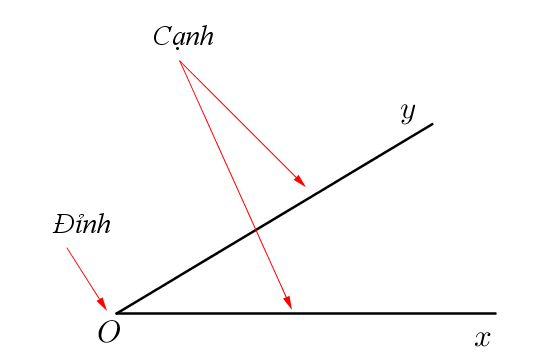
\includegraphics[width= 0.5\linewidth]{vd-30-1}
	\end{center}
	\i Góc  $xOy$, kí hiệu $\widehat{xOy}$ (hay $\widehat{yOx},\,\widehat{O}$) gồm hai tia chung gốc là $Ox$ và $Oy$. Điểm $O$ là đỉnh của góc $xOy$. Hai tia $Ox,\,Oy$ là cạnh của góc $xOy$.
\end{enumerate}
\subsubsection{Điểm trong của góc}
\begin{enumerate}[--,leftmargin=*]
	\immini{\i Ta gọi $A$ là một điểm trong của góc $xOy$
	\i Các điểm nằm trên hai cạnh của góc chẳng hạn như $C$ và các điểm như điểm $B$ không phải là điểm trong của góc $xOy$.}{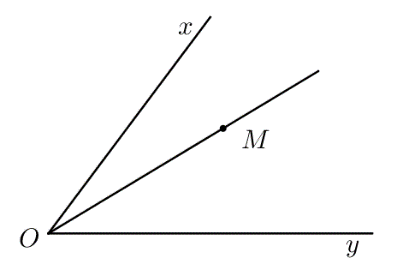
\includegraphics[width= 0.5\linewidth]{vd-30-2}}
\end{enumerate}
\subsubsection{Số đo góc}
\subsubsection*{a. Số đo góc}
\begin{enumerate}[--,leftmargin=*]
	\i Muốn đo góc $xOy$, ta đặt thước đo góc sao cho tâm của thước trùng với $O$, tia $Ox$ đi qua vạch $0$. Khi đó tia $Oy$ đi qua vạch chỉ số đo của góc. Trên hình dưới đây, ta thấy $Oy$ đi qua vạch 110. Vậy góc $xOy$ có số đo là 110 độ. Ta viết $\widehat{xOy}={{110}^\circ}$.\\
	\immini{$\widehat{xOy} = 110^\circ$\\
		(Đọc số ở vòng cung lớn)}{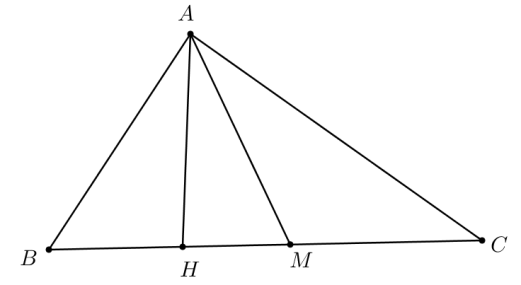
\includegraphics[width= 0.5\linewidth]{vd-30-3}}
	\i Mỗi góc có một số đo. Số đo của một góc không vượt quá ${{180}^\circ}$.
\end{enumerate}
\subsubsection*{b. So sánh góc}
So sánh hai góc bằng cách so sánh số đo của chúng.
\begin{enumerate}[--,leftmargin=*]
	\i Hai góc $\widehat{xAy}$ và $\widehat{vOt}$ có số đo bằng nhau.
	\begin{center}
		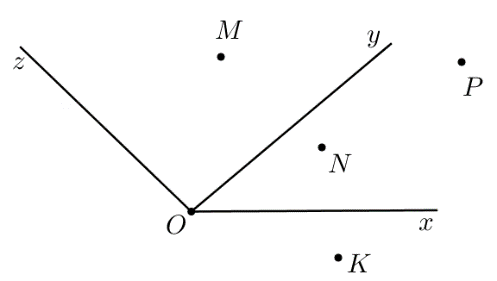
\includegraphics[width= 0.5\linewidth]{vd-30-4}
	\end{center}
	\i Góc $\widehat{tOz}$ có số đo lớn hớn $\widehat{CAB}$, ta viết $\widehat{tOz}>\widehat{CAB}$, ta nói $\widehat{tOz}$ lớn hơn $\widehat{CAB}$.
	\begin{center}
		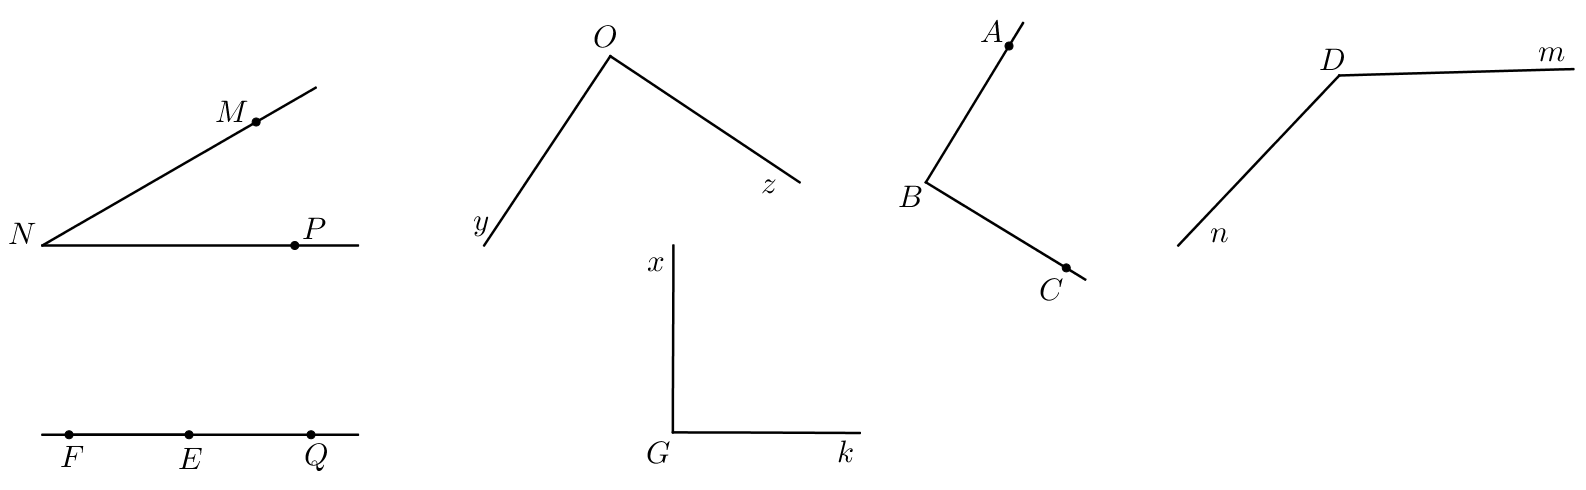
\includegraphics[width= 0.5\linewidth]{vd-30-5}
	\end{center}
\end{enumerate}
\subsubsection*{c. Các góc đặc biệt}
\begin{enumerate}[--,leftmargin=*]
	\i Góc có số đo bằng ${{90}^\circ}$ là góc vuông.
	\i Góc bẹt có số đo bằng ${{180}^\circ}$.
	\i Góc nhỏ hơn góc vuông là góc nhọn.
	\i Góc lớn hơn góc vuông, nhỏ hơn góc bẹt là góc tù.
\end{enumerate}
\subsection{THỰC HÀNH GIẢI TOÁN}
\begin{vd}
	Đọc tên các góc, ghi đỉnh và các cạnh của mỗi góc. 
	\begin{center}
		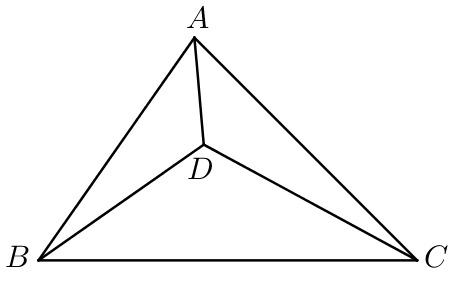
\includegraphics[width= 0.5\linewidth]{vd-30-6}
	\end{center}
	\loigiai{
		\begin{enumerate}[+,leftmargin=*]
			\i Góc $\widehat{xOy}$: đỉnh $O$, cạnh $Ox,Oy$.
			\i Góc $\widehat{vOt}$: đỉnh $O$, cạnh $Ov,Ot$.
		\end{enumerate}
	}
\end{vd}
\begin{vd}
	Xác định các điểm nằm trong góc $\widehat{mOn}$ và các điểm không nằm trong góc $\widehat{mOn}$.
	\begin{center}
		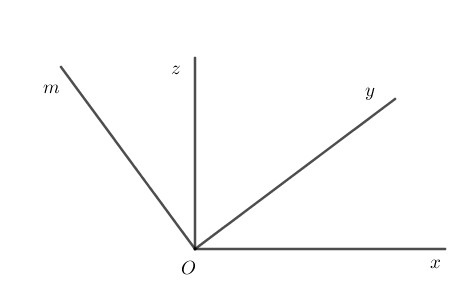
\includegraphics[width= 0.5\linewidth]{vd-30-7}
	\end{center}
	\loigiai{
		\begin{enumerate}[+,leftmargin=*]
			\i Điểm nằm trong góc $\widehat{mOn}$: $M,N,T$.
			\i Điểm không nằm trong góc $\widehat{mOn}$: $B,V,A$.
		\end{enumerate}
	}
\end{vd}
\begin{vd}
	Liệt kê các góc có trong hình vẽ sau. Em hãy đo các góc đó và so sánh các góc.
	\begin{center}
		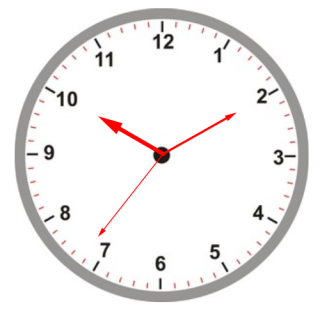
\includegraphics[width= 0.5\linewidth]{vd-30-8}
	\end{center}
	\loigiai{
		Các góc: $\widehat{zOy},\widehat{xOz},\widehat{xOy}$\\
		$\widehat{zOy}={{60}^\circ},\,\,\,\,\widehat{xOz}={{120}^\circ},\,\,\,\,\widehat{xOy}={{180}^\circ}$\\
		$\widehat{zOy}<\widehat{xOz}<\widehat{xOy}$.
	}
\end{vd}
\subsection{MỞ RỘNG KIẾN THỨC}
\subsubsection{Vẽ góc khi có số đo cho trước bằng thước đo góc}
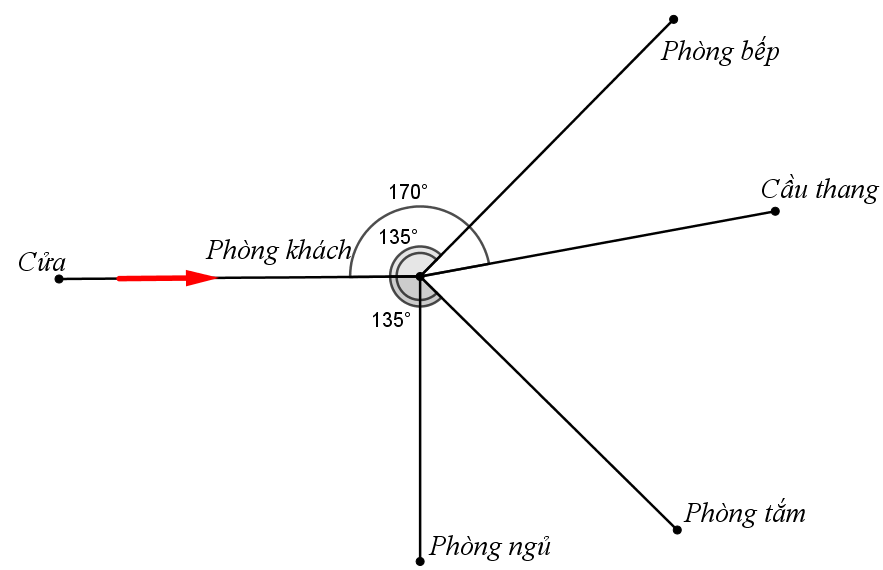
\includegraphics[width= 0.5\linewidth]{vd-30-9}
\begin{enumerate}[+,leftmargin=*]
	\i Vẽ góc $\widehat{xOy}={{m}^\circ}\left( 0<m<180 \right)$
	\begin{enumerate}[--,leftmargin=*]
		\i Vẽ tia $Ox$
		\i Đặt thước đo góc sao cho tâm thước trùng với gốc $O$ của tia $Ox$ và tia $Ox$ đi qua vạch ${{0}^\circ}$.
		\i Kẻ tia $Oy$ qua vạch ${{m}^\circ}$ của thước.
	\end{enumerate}
\end{enumerate}
\subsubsection{Công thức cộng góc}
Cho điểm $M$ nằm trong $\widehat{xOy}$. Khi đó: $\widehat{xOM}+\widehat{MOy}=\widehat{xOy}$.
\subsubsection{Công thức tính số góc tạo thành từ các tia chung gốc cho trước.}
Cho $n$ tia phân biệt chung gốc. Cứ 2 tia chung gốc tạo thành một góc. Khi đó số góc tạo bởi 2 trong $n$ tia trên là: $\dfrac{n(n-1)}{2}$ góc
\subsection{BÀI TẬP TỰ LUYỆN}
\Opensolutionfile{loigiaichung}[loigiaichuong30]
\subsubsection*{Mức độ cơ bản}
\begin{bt}
	\immini{Bài 1. Quan sát hình bên và: 
		\begin{enumerate}[a),leftmargin=*]
			\i Đọc tên các góc trong hình vẽ. Mỗi góc, hãy cho biết các đỉnh và các cạnh của nó.
			\i Xác định điểm nằm trong, nằm ngoài của mỗi góc trên.
	\end{enumerate}}{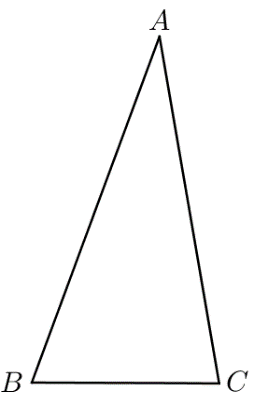
\includegraphics[width= 0.5\linewidth]{vd-30-10}}
	\begin{loigiaichuong30}
		\begin{enumerate}[a),leftmargin=*]
			\i Các góc trong hình vẽ:
			\begin{enumerate}[--,leftmargin=*]
				\i $\widehat{xOy}$: đỉnh $O$; cạnh $Ox,Oy$.
				\i $\widehat{yOz}$: đỉnh $O$; cạnh $Oy,Oz$.
				\i $\widehat{xOz}$: đỉnh $O$; cạnh $Ox,Oz$.
			\end{enumerate}
			\i Các điểm nằm trong góc $\widehat{xOy}:\,\,N,P$.
			\begin{enumerate}[--,leftmargin=*]
				\i Các điểm nằm ngoài góc $\widehat{xOy}:\,\,M,K$.
				\i Các điểm nằm trong góc $\widehat{yOz}:\,\,M$.
				\i Các điểm nằm ngoài góc $\widehat{yOz}:\,\,N,P,K$.
				\i Các điểm nằm trong góc $\widehat{xOz}:\,\,M,N,P$.
				\i Các điểm nằm ngoài góc $\widehat{xOz}:\,\,K$.
			\end{enumerate}
		\end{enumerate}
	\end{loigiaichuong30}
\end{bt}
\begin{bt}%%%%%%%%
	Viết tên các góc có đỉnh $A;M;H$ có trong hình vẽ.
	\begin{center}
		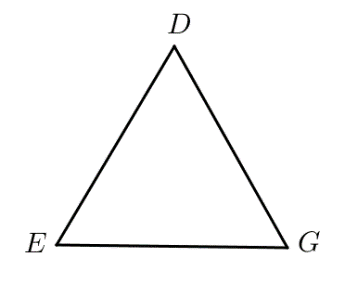
\includegraphics[width= 0.5\linewidth]{vd-30-11}
	\end{center}
	\begin{loigiaichuong30}
		Các góc có đỉnh $A:\,\,\widehat{BAH},\widehat{BAM},\widehat{BAC},\widehat{HAM},\widehat{HAC},\widehat{MAC}$.
		
		Các góc có đỉnh $M:\,\,\widehat{AMC},\widehat{AMH},\widehat{AMB}$.
		
		Các góc có đỉnh .
	\end{loigiaichuong30}
\end{bt}
\begin{bt}
	Quan sát các hình sau:
	\begin{center}
		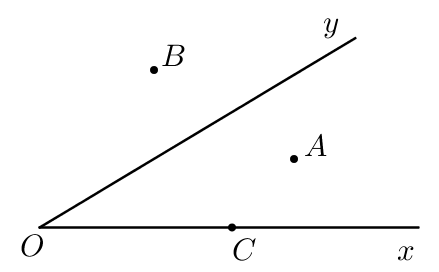
\includegraphics[width= 0.5\linewidth]{vd-30-12}
	\end{center}
	\begin{enumerate}[a),leftmargin=*]
		\i Ước lượng bằng mắt xem góc nào là góc nhọn, góc vuông, góc tù, góc bẹt.
		\i Dùng êke để kiểm tre lại kết quả của câu a.
		\i Dùng thước đo góc để tìm số đo của mỗi góc trên.
	\end{enumerate}
	\begin{loigiaichuong30}
		\begin{enumerate}[a),leftmargin=*]
			\i Góc nhọn: $\widehat{MNP}$; góc tù: $\widehat{mDn}$; góc vuông: $\widehat{ABC},\widehat{xGk},\widehat{yOz}$; góc bẹt: $\widehat{FEQ}$.
			\i Dùng êke kiểm tra lại kết quả.
			\i Dùng thước đo góc: $\widehat{MNP}={{30}^\circ},\widehat{yOz}={{90}^\circ},\widehat{ABC}={{90}^\circ},\widehat{mDn}={{135}^\circ},\widehat{FEQ}={{180}^\circ},\widehat{xGk}={{90}^\circ}$
		\end{enumerate}
	\end{loigiaichuong30}
\end{bt}
\begin{bt}
	Quan sát hìn ảnh của mặt đồng hồ, em hãy tìm hai thời điểm mà góc tạo bởi kim giờ và kim phút là:
	
	\begin{tabularx}{\textwidth}{*{2}{Z}}
		a) góc nhọn	&b) góc tù\\
		c) góc bẹt	&d) góc vuông
	\end{tabularx}
	\begin{loigiaichuong30}
		Góc tạo bởi kim giờ và kim phút là:
		\begin{enumerate}[a),leftmargin=*]
			\i góc nhọn: lúc 2 giờ, 11 giờ.
			\i góc tù: lúc 4 giờ, 5 giờ.
			\i góc bẹt: lúc 6 giờ.
			\i góc vuông: lúc 3 giờ, 9 giờ.
		\end{enumerate}
	\end{loigiaichuong30}
\end{bt}
\begin{bt}
	Em hãy nêu các hình ảnh thực tế về góc.	
	\begin{loigiaichuong30}
		Hình ảnh thực tế về góc:
		\begin{enumerate}[+,leftmargin=*]
			\i Góc tạo bởi kim phút và kim giây của đồng hồ.
			\i Góc tạo bởi cái bóng và cây cột giữa trời nắng và mặt đất.
		\end{enumerate}
	\end{loigiaichuong30}
\end{bt}
\begin{bt}
	\immini{Quan sát hình vẽ và cho biết: 
		\begin{enumerate}[a),leftmargin=*]
			\i Số góc có trong hình vẽ.
			\i Nêu tên các góc ở câu a và cho biết số đo của mỗi góc. 
	\end{enumerate}}{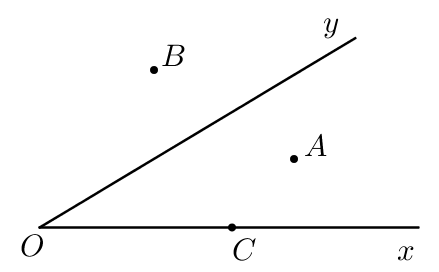
\includegraphics[width= 0.5\linewidth]{vd-30-12}}
	\begin{loigiaichuong30}
		\begin{enumerate}[a),leftmargin=*]
			\i Có 12 góc.
			\i $\widehat{ABC}={{55}^\circ};\widehat{BAC}={{80}^\circ};\widehat{ACB}={{45}^\circ};\widehat{ADB}={{110}^\circ};\widehat{BDC}={{130}^\circ};\widehat{ADC}={{120}^\circ}$
			$\widehat{CBD}={{25}^\circ},\widehat{DBA}={{20}^\circ},\widehat{BCD}={{20}^\circ},\widehat{DCA}={{25}^\circ},\widehat{BAD}={{40}^\circ},\widehat{CAD}={{40}^\circ}$
		\end{enumerate}
	\end{loigiaichuong30}
\end{bt}
\begin{bt}
	\begin{enumerate}[a),leftmargin=*]
		\i Vẽ tam giác $ABC$ bất kì. Ước lượng số đo các góc của tam giác rồi đo và cho biết tổng 3 góc trong tam giác đó là bao nhiêu?
		\i Vẽ tam giác đều $DEG$. Đo các góc của tam giác.
		\i Vẽ $\Delta MNP$ có $\widehat{M}={{90}^\circ},MP=MN$. Đo các góc $\widehat{B}$ và $\widehat{C}$.
	\end{enumerate}
	\begin{loigiaichuong30}
		\begin{enumerate}[a),leftmargin=*]
			\i Tam giác $ABC$ có:
			\begin{enumerate}[--,leftmargin=*]
				\i $\widehat{BAC}={{30}^\circ}$
				\i $\widehat{ABC}={{70}^\circ}$
				\i $\widehat{ACB}={{80}^\circ}$
				\i $\widehat{BAC}+\widehat{ABC}+\widehat{ACB}={{180}^\circ}$
			\end{enumerate}
			\i Tam giác đều $DEG$ có:
			\begin{enumerate}[--,leftmargin=*]
				\i $\widehat{D}={{60}^\circ}$
				\i $\widehat{G}={{60}^\circ}$
				\i $\widehat{E}={{60}^\circ}$
			\end{enumerate}
		\end{enumerate}
	\end{loigiaichuong30}
\end{bt}
\begin{bt}
	Tính góc tạo bởi kim giờ và kim phút của đồng hồ lúc 4 giờ, 9 giờ, 11 giờ, 6 giờ.
	\begin{loigiaichuong30}
		Góc tạo bởi kim giờ và kim phút của đồng hồ:
		\begin{enumerate}[--,leftmargin=*]
			\i lúc 4 giờ: ${{120}^\circ}$
			\i lúc 9 giờ: ${{90}^\circ}$
			\i lúc 11 giờ: ${{30}^\circ}$
			\i lúc 6 giờ: ${{180}^\circ}$
		\end{enumerate}
	\end{loigiaichuong30}
\end{bt}
\begin{bt}
	Quan sát mặt đồng hồ ở hình bên và cho biết trong các vạch chỉ số trên mặt đồng hồ, những vạch số nào nằm trong góc tạo bởi
	\immini{\begin{enumerate}[a),leftmargin=*]
			\i Kim giây và kim phút.
			\i Kim giờ và kim phút.
	\end{enumerate}}{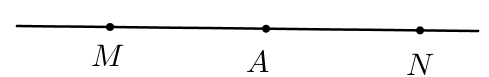
\includegraphics[width= 0.5\linewidth]{vd-30-13}}
	\begin{loigiaichuong30}
		Những vạch số nằm trong góc tạo bởi
		\begin{enumerate}[a),leftmargin=*]
			\i kim giây và kim phút: 7; 6; 5; 4; 3
			\i kim giờ và kim phút: 11; 12; 1; 1
		\end{enumerate}
	\end{loigiaichuong30}
\end{bt}
\begin{bt}%%%%%
	\immini{Quan sát hình vẽ bên
		\begin{enumerate}[a),leftmargin=*]
			\i Đọc tên các góc có trong hình vẽ.
			\i Đo và cho biết góc nhọn, góc vuông, góc tù.
			\i Viết tên các cặp góc có số đo bằng nhau.
	\end{enumerate}}{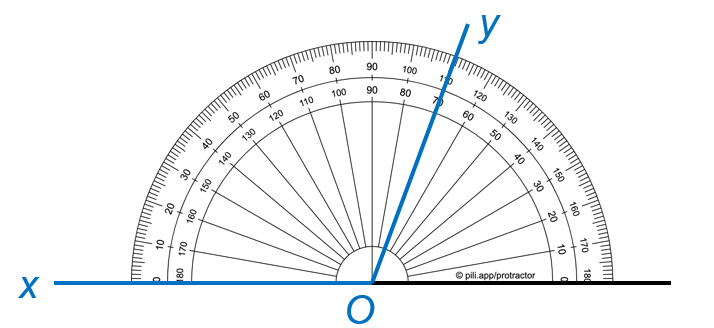
\includegraphics[width= 0.5\linewidth]{vd-30-14}}
	\begin{loigiaichuong30}
		\begin{enumerate}[a),leftmargin=*]
			\i Các góc có trong hình vẽ: $\widehat{mOz},\widehat{mOy},\widehat{mOx},\widehat{zOy},\widehat{zOx},\widehat{yOx}$
			\i Góc nhọn: $\widehat{mOz},\widehat{zOy},\widehat{yOx}$; góc vuông: $\widehat{mOn},\widehat{xOz}$; góc tù: $\widehat{xOm}$.
		\end{enumerate}
	\end{loigiaichuong30}
\end{bt}
\begin{bt}
	Điền từ thích hợp vào chỗ chấm. Đi từ cửa đến phòng khách rẽ trái theo góc ${{135}^\circ}$ thì đến \ldots 
	\begin{center}
		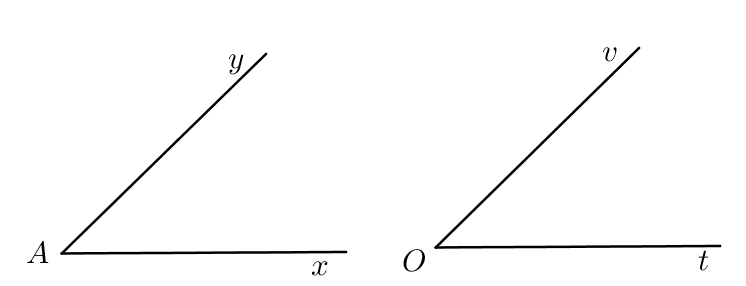
\includegraphics[width= 0.5\linewidth]{vd-30-15}
	\end{center}
	\begin{tabularx}{\textwidth}{*{4}{Y}}
	A. Phòng bếp&	B. Cầu thang&	C. Phòng tắm	&D. Phòng ngủ
	\end{tabularx}
	\begin{loigiaichuong30}
		A. Phòng bếp.
	\end{loigiaichuong30}
\end{bt}
\subsubsection{Mức độ nâng cao}
\begin{bt}
	Cho năm tia phân biệt chung gốc $Ox,Om,Oy,On,Ot$. Số góc tạo bởi hai trong năm tia là bao nhiêu
	\begin{loigiaichuong30}
		Số góc tạo bởi hai trong năm tia là:
		\begin{enumerate}[--,leftmargin=*]
			\i Số góc tạo bởi tia $Ox$ với 1 trong 4 tia còn lại là: 4 góc.
			\i Số góc tạo bởi tia $Om$ với 1 trong 3 tia còn lại (không kể $Ox$) là: 3 góc.
			\i Số góc tạo bởi tia $Oy$ với 1 trong 2 tia còn lại (không kể $Ox,Oy$) là: 2 góc.
			\i Số góc tạo bởi tia $On$ với tia $Ot$ còn lại là: 1 góc.
		\end{enumerate}
		Vậy số góc tạo thành là: $4+3+2+1=10$ góc.
	\end{loigiaichuong30}
\end{bt}
\begin{bt}
	Cho bốn tia chung gốc $Ox,Om,Oy,On$, trong đó hai tia $Oy,On$ đối nhau. Số góc tạo bởi hai trong bốn tia không kể góc bẹt là bao nhiêu?
	\begin{loigiaichuong30}
		Xét góc tạo bởi tia thứ nhất với 1 trong 3 tia còn lại có 3 góc.\\
		Xét góc tạo bởi tia thứ 2 với 1 trong 2 tia còn lại có 2 góc.\\
		Xét góc tạo bởi tia thứ 3 với 1 tia còn lại có 1 góc.\\
		Do đó, số góc tạo thành: $3+2+1=6$ góc.\\
		Vì $Oy,On$ là hai tia đối nên tạo thành 1 góc bẹt.\\
		Vậy số góc tạo bởi 2 trong 4 tia không kể góc bẹt là: $6-1=5$ góc.
	\end{loigiaichuong30}
\end{bt}
\begin{bt}
	Cho $n$ tia chung gốc, biết chúng tạo thành 21 góc. Tìm giá trị của $n$.
	\begin{loigiaichuong30}
		Số góc tạo bởi tia thứ nhất với 1 trong $n-1$ tia còn lại là $n-1$ góc.\\
		Số góc tạo bởi tia thứ hai với 1 trong $n-2$ tia còn lại là $n-2$ góc.\\
		\ldots \\
		Số góc tạo bởi tia thứ $n-1$ với tia thứ $n$ là 1 góc.\\
		Do đó, tổng số góc là: $1+2+...+n-2+n-1=n\cdot\left( n-1 \right):2$\\
		Ta có: $n\cdot\left( n-1 \right):2=21\Rightarrow n\cdot\left( n-1 \right)=42$\\
		mà $42=7\cdot6$ nên $n=7$
	\end{loigiaichuong30}
\end{bt} 
\begin{bt}
	Cho $n$ tia chung gốc $O$. Sau khi xóa một tia đi qua gốc $O$ thì số góc giảm đi 10. Tìm giá trị của $n$.
	\begin{loigiaichuong30}
		Ta có:\\
		Xóa 1 tia gốc $O$ thì số góc giảm đi 10\\
		Khi chưa xóa tia, số góc tạo bởi tia đó với $n-1$ tia còn lại là $n-1$ góc.\\
		Số góc giảm đi 10 khi xóa 1 tia nên: $n-1=10 \Rightarrow n=11$.
	\end{loigiaichuong30}
\end{bt}
\begin{bt}
	Cho $\widehat{MAN}$ là góc bẹt và tia $AT$. Biết $\widehat{MAT}-\widehat{NAT}={{8}^\circ}$. Tính $\widehat{NAT}$.
	\begin{loigiaichuong30}
		Ta có: $\widehat{MAN}$ là góc bẹt nên $\widehat{MAN}={{180}^\circ}$.\\
		$\widehat{MAT}+\widehat{NAT}=\widehat{MAN}\Rightarrow \widehat{MAT}+\widehat{NAT}={{180}^\circ}$\\
		mà  $\widehat{MAT}-\widehat{NAT}={{8}^\circ}$  nên:
		$\widehat{MAT}=\left({{180}^\circ}+{{8}^\circ}\right):2={{94}^\circ}$ \\ 
		$\widehat{NAT}=\left({{180}^\circ}-{{8}^\circ}\right):2={{86}^\circ}$ \\ 
	\end{loigiaichuong30}
\end{bt}
\Closesolutionfile{loigiaichung}

%	\def\i{\item}
\graphicspath{{../pictures/vande31/}}
\chapter{Chương 5}
\section{Ôn tập chương}
\subsection{Kiến thức cần nhớ}
\begin{tabular}{|c|p{2.2cm}|p{0.5\linewidth}|p{0.25\linewidth}|}
	\hline
	STT	&Nội dung& 	Kiến thức cần nhớ& 	Các dạng bài tập thường gặp\\
	\hline
	1&	Điểm Đường thẳng Tia& \begin{enumerate}[--,leftmargin=*]
		\i Điểm là dấu chấm nhỏ , kí hiệu bằng chữ in hoa ($A$, $B$, $C$, ...)
		\i Đường thẳng không bị giới hạn về hai phía, thường kí hiệu bằng chữ thường ($a$, $b$, $c$, ...)
		
		$M\in d;\,N\notin d$
		\i Tia là hình gồm điểm $O$ và nửa đường thẳng được chia bởi điểm $O$
		
		Tia $Ox,\,Oy$
		\i Hai tia chung gốc tạo thành một đường thẳng là hai tia đối nhau
		$Ox,\,Oy$là hai tia đối nhau
	\end{enumerate} &
	\begin{enumerate}[--,leftmargin=*]
		\i Vẽ hình theo yêu cầu 
		\i Xác định số đường thẳng, đoạn thẳng, tia , ...
	\end{enumerate}\\
	\hline
	2	&Ba điểm thẳng hàng& \begin{enumerate}[--,leftmargin=*]
		\i Ba điểm thẳng hàng là 3 điểm cùng thuộc 1 đường thẳng
		\i Trong ba điểm thẳng hàng có một và chỉ một điểm nằm giữa 2 điểm còn lại 
		\begin{enumerate}[+,leftmargin=*]
			\i Điểm $C$ nằm giữa $A$ và $B$
			\i $A$và $B$ nằm khác phía so với $C$ 
			\i $A$ và $C$ nằm cùng phía với $B$;
			\i $C$ và $B$ nằm cùng phía với $A$.
		\end{enumerate}
	\end{enumerate}&
	\begin{enumerate}[--,leftmargin=*]
		\i Nhận xét ba điểm thẳng hàng 
		\i Vẽ hình theo yêu cầu 
		\i Bài toán trồng cây
	\end{enumerate}\\
	\hline
	3&	Vị trí tương đối giữa hai đường thẳng&
	\begin{enumerate}[--,leftmargin=*]
		\i Hai đường thẳng $a,\,b$ có các trường hợp 
		\begin{enumerate}[+,leftmargin=*]
			\i $a \parallel b$: $a$ và $b$ không có điểm chung
			\i $a$ cắt $b$: $a$ và $b$  có 1 điểm chung
			\i $a$$\underset{\scriptscriptstyle-}{=}$$b$: $a$ và $b$ có vô số điểm chung.
		\end{enumerate}
		Chú ý: hai đường thẳng phân biệt có thể song song hoặc cắt nhau.
	\end{enumerate}&
	\begin{enumerate}[--,leftmargin=*]
		\i Nhận biết đường thẳng song song, cắt nhau, trùng nhau
		\i Vẽ hình theo yêu cầu
	\end{enumerate}\\
	4	&Độ dài đoạn thẳng 
	Trung điểm của đoạn thẳng&
	\begin{enumerate}[--,leftmargin=*]
		\i Đoạn thẳng $AB$ là hình giữa hai điểm $A,\,B$ và các điểm nằm giữa $A$, $B$, $A$ và $B$ là hai đầu mút 
		\i Nếu $M$ nằm giữa $A$ và $B$ thì $AM+MB=AB$
		\i Nếu $I$ nằm giữa $A$ và $B$ , và $IA=IB$ thì $I$ là trung điểm của $AB$
	\end{enumerate}&
	\begin{enumerate}[--,leftmargin=*]
		\i Nhận biết đoạn thẳng 
		\i Tính, so sánh độ dài đoạn thẳng 
		\i Chứng minh trung điểm đoạn thẳng
	\end{enumerate}\\
	 \hline
	5&	Góc - Số đo góc	&
	\begin{enumerate}[--,leftmargin=*]
		\i Góc là hình giữa hai tia chung gốc.
		Gốc chung giữa 2 tia là đỉnh của góc Hai tia là hai cạnh của góc. 
		Kí hiệu : $\widehat{xOy}$
		\i Quy tắc cộng góc: Nếu điểm $M$ nằm trong góc $\widehat{xOy}$ thì $\widehat{xOM}+\widehat{MOy}=\widehat{xOy}$
		\i Góc vuông  
		
		\i Góc nhọn
		
		\i Góc tù
		
		\i Góc bẹt  
	\end{enumerate} & 
	\begin{enumerate}[--,leftmargin=*]
		\i Đọc tên góc, viết kí hiệu 
		\i Đo góc 
		\i Vẽ góc
		\i Tính số đo góc
	\end{enumerate}
\end{tabular}

%B. Bài tập tự luyện 
%Bài 1. Em hày hoàn thành 10 câu trắc nghiệm sau 
%1) Trong các câu sau , câu nào đúng 
%A. Hai tia chung gốc thì đối nhau
%B. Hai tia chung gốc cùng nằm trên 1 đường thẳng thì đối nhau 
%C. Hai tia chung gốc tạo thành 1 đường thẳng thì đối nhau
%D. Hai tia chung gốc tạo thành một nửa đường thẳng thì đối nhau
%2) Ba đường thẳng A, B, C thẳng hàng khi 
%A. A, B, C thuộc ba đường thẳng phân biệt
%B. A, B, C thuộc ba đưởng thẳng song song 
%C. A, B, C thuộc cùng một đường thẳng bất kì 
%D. Cả 3 đáp án trên đều đúng
%3) Khẳng định nào sai 
%A. Góc nhọn nhỏ hơn góc vuông 
%B. Góc tù nhỏ hơn góc nhọn 
%C. Góc bẹt nhỏ hơn góc vuông
%D. Góc vuông nhỏ hơn góc tù 
%4) Đo góc $\widehat{xOy}$
%
%A. $45{}^\circ $	B. $30{}^\circ $	C. $50{}^\circ $	D. $40{}^\circ $
%
%5) Có bao nhiêu bộ ba điểm thẳng hàng trong hình sau 
%
%A. 10	B. 11	C. 12	D. 13
%6) Trong hình vẽ dưới đây , số đường thẳng đi qua D và không đi qua E là
%
%A. 4	B. 3	C. 2	D. 1
%7) Có bao nhiêu cặp đường thẳng song song trong hình vẽ
%
%A. 6	B. 5	C. 4	D. 7
%8) Có bao nhiêu bộ ba điểm thẳng hàng trong hình vẽ 
%
%A. 2	B. 4	C. 5	D. 3
%9) Nếu điểm B nằm trong góc $\widehat{xOy}$ thì
%A. $\widehat{xOB}+\widehat{xOy}=\widehat{yOB}$		B. $\widehat{xOB}-\widehat{yOB}=\widehat{xOy}$
%C. $\widehat{xOB}+\widehat{yOB}=\widehat{xOy}$		D. $\widehat{yOB}+\widehat{xOy}=\widehat{xOB}$
%10) Ta có thể xem kim giờ và kim phút của đồng hồ là hai tia chung gốc ( gốc trùng với trục quay của hai kim ). Tại mỗi thởi điểm, hai kim tạo thành một góc. Quan sát các đồng hồ sau và sắp xếp các hình đồng hồ theo thứ tự giảm dần số đo của góc tạo bởi kim giờ và kim phút.
%Hình 1		Hình 2	Hình 3	Hình 4
%A. Hình 1, hình 2, hình 3, hình4
%B. Hình 1, hình 2, hình 4, hình 3
%C. Hình 3, hình 2, hình 4, hình 1  
%D. Hình 3, hình 4, hình 1, hình 2
%Bài 2. Ghép mỗi ý ở cột Hình hình học với hình vẽ tương ứng ở cột Hình vẽ
%Hình vẽ
%A)    
%B)        
%C)       
%D) 
%E)
%F) 
%G) 
%H)    
%L)      
%M)      
%N) 
%
%
%Hình hình học
%(1) Điểm $A$
%(2) Đường thẳng đi qua hai điểm $A$và $B$
%(3) Đoạn thẳng $MN$
%(4) Tia $At$
%(5) Điểm nằm trên đường thẳng  
%(6) Hai đường thẳng cắt nhau
%(7) Điểm nằm ngoài đường thẳng 
%(8) Hai đường thẳng song song
%(9) Ba điểm không thẳng hàng 
%(10) Ba điểm thẳng hàng
%(11) Đoạn thẳng $AB$ có độ dài bằng $3cm$
%(12) Điểm nằm $M$giữa hai điểm $C$và $D$
%
%
%
%
%
%
%
%
%Bài 3. Cho hình vẽ 
%
%a) Kể tên các tia đối nhau 
%b) Kể tên các cặp đường thẳng cắt nhau (các cặp đường thẳng trùng nhau chỉ tính 1 lần)
%c) Kể tên các bộ ba điểm thẳng hàng
%Bài 4. Cho hình chữ nhật \[ABCD\] và các điểm $M,N,H$ như hình vẽ. 
%a) Kể tên các góc đỉnh $M$
%b) Đo các góc $\widehat{ANM};\,\widehat{NMD};\,\widehat{DMC};\,\widehat{ADM}$
%c) Kể tên các góc vuông trong hình vẽ 
%d) Kể tên các góc nhọn trong hình vẽ.
%Bài 5. Em hãy tìm ít nhất 3 biển báo giao thông (ghi rõ tên biển báo) có hình ảnh 2 đường thẳng song song, 3 biển báo có hình ảnh 2 đường thẳng cắt nhau.
%Bài 6. Vẽ hình theo diễn đạt (mỗi hình 1 ý)
%a) Vẽ hai tia $Ox,\,Oy$ phân biệt và không đối nhau
%b) Vẽ đường thẳng $d$// ${d}'$, đường thẳng $c$cắt $d$ và  ${d}'$ lần lượt tại M và N
%c) Vẽ góc $\widehat{mAt}$$=60{}^\circ $, lấy điểm P, Q nằm trong góc $\widehat{mAt}$ sao cho $A,\,P,\,Q$ không thẳng hàng. Đo góc $\widehat{PAm};\,\widehat{tAQ}$
%Bài 7. Trên tia $Ox$ lấy hai điểm $A$ và $B$ sao cho $OA=3cm$, $OB=6cm$
%a) So sánh $OA$ và $OB$
%b) Tính độ dài $AB$ 
%c) Điểm $A$ có là trung điểm của $OB$ không? Vì sao? 
%Bài 8. Trên tia $Ox$ lấy $A$ và $B$ sao cho $OA=8cm$, $OB=4cm$ 
%a) Tính độ dài $AB$
%b) Trên tia đối của tia $Ox$ lấy điểm $C$ sao cho $OC=4cm$. Tính $AC,\,BC$
%c) $O$ có là trung điểm của $BC$ không? Vì sao?
%Bài 9. Vẽ đoạn thẳng $AB=10cm$. Gọi $I$là trung điểm của $AB$. Trên đoạn thẳng $AB$lấy $M,\,N$sao cho $AM=BN=2cm$. Chứng minh $I$ là trung điểm của $MN$
%
%Mức độ nâng cao 
%Bài 10. Vẽ đoạn thẳng $MN=6cm$. Trên tia $MN$lấy điểm $O$ sao cho$NO=2cm$. Tính $OM$
%Bài 11. Cho đoạn thẳng $AB$ và $M$ là trung điểm của nó. Gọi $C$là điểm nằm giữa $M$ và $B$. Hãy chứng tỏ rằng $CM=\frac{CA-CB}{2}$
%Bài 12: Vòng quay mặt trời trong khu vui chơi có đường kính là $66m,$ chiều cao của trục vòng quay so với mặt đất là $43m.$Hỏi điểm cao nhất và điểm thấp nhất của vòng quay nằm ở độ cao nào so với mặt đất?
%
%Bài 13: Cho $2022$ đường thẳng cắt nhau từng đôi một. Hỏi có nhiều nhất bao nhiêu giao điểm được tạo thành?
%Bài 14: Vẽ góc $\widehat{xOy}={{60}^{0}}.$ Vẽ tia \[Oz\] sao cho $\widehat{xOz}={{30}^{0}}.$ Tính góc $\widehat{y\text{O}z}?$
%Bài 15: Cho $1998$ tia gốc $O.$ Sau khi vẽ thêm hai tia đi qua gốc $O.$ Số đo tăng  thêm tại đỉnh $O$ là bao nhiêu?
%Bài 16: Cho $n$ điểm không có ba điểm nào thẳng hàng. Nếu ta vẽ thêm hai điểm (không tạo ra ba điểm thẳng hàng) thì số đường thẳng nối hai trong số các điểm đó tăng lên $13$ đường thẳng. Tìm $n.$
%Bài 17: Cho điểm $M$nằm giữa hai điểm $A$ và $B.$ Điểm $I$là trung điểm của đoạn thẳng $AB$ và $5AB=8AM.$ Biết $MI=2cm.$ Tính $AB.$ 
%C. Hướng dẫn giải và đáp số
%Bài 1. 
%1) C	2) C	3) B	4) A	5) A
%6) D	7) A	8) D	9) C	10) D
%Bài 2. 
%$\left( 1 \right)-B$	$\left( 4 \right)-E$	$\left( 7 \right)-$trống	$\left( 10 \right)-H$
%$\left( 2 \right)-C$	$\left( 5 \right)-G$	$\left( 8 \right)-F$	$\left( 11 \right)-M$
%$\left( 3 \right)-A$	$\left( 6 \right)-D$	$\left( 9 \right)-N$	$\left( 12 \right)-L$
%Bài 3. 
%a) Các tia đối nhau là: $Ax$và $Ay$; $Cx$ và $Cy$; $Dx$ và $Dy$
%b) Các đường thẳng cắt nhau là: $AO$và $BA$; $BE$và $BA$
%c) Các bộ ba điểm thẳng hàng là: $A,C,D$; $B,F,A$
%Bài 4. 
%a) Các góc có đỉnh $M$ là: $\widehat{BMC};\widehat{NMH};\widehat{BMN};\widehat{HMC}$
%b) $\widehat{ANM}=120{}^\circ ;\widehat{DMC}=35{}^\circ ;\widehat{NMD}=120{}^\circ ;\widehat{ADM}=35{}^\circ $
%c) Các góc vuông trong hình vẽ là: $\widehat{BA\text{D}};\widehat{A\text{D}C};\widehat{ABC};\widehat{BC\text{D}}$
%d) Các góc nhọn trong hình vẽ là: $\widehat{BMN};\widehat{HMC};\widehat{MCH};\widehat{HCD};\widehat{CDH};\widehat{DHC};\widehat{ADM}$
%Bài 5. 
%- Các biển báo có 2 đường thẳng song song là: Nhường đường cho xe ngược chiều qua đường hẹp; Đường hai chiều; Giao nhau với đường hai chiều
%- Các biển báo có 2 đường thẳng cắt nhau là: Cấm rẽ trái; cấm rẽ phải; cấm đỗ xe ngang lề
%
%Bài 6. 
%a)                                                 b)                                               c)
%
%$\widehat{PAm}=40{}^\circ ;\widehat{QAt}=35{}^\circ $
%Bài 7. 
%
%Vì $A$ nằm giữa $O,B$ nên ta có: $OA<OB$
%Lại có: 
%$OA+AB=OB\Rightarrow AB=OB-OA=6-3=3\left( cm \right)$
%Vì $A$ nằm giữa $O,B$ và $OA=AB=\frac{OB}{2}=3\left( cm \right)$ nên $A$ là trung điểm của $AB$
%Bài 8. 
%
%a) Vì $B$ nằm giữa $O,A$ nên ta có: $OB+AB=OA$
%$\Rightarrow AB=OA-OB=8-4=4\left( cm \right)$
%b) Vì $O$ nằm giữa $A,C$ nên ta có: $AC=OA+OC=8+4=12\left( cm \right)$
%Vì $O$ nằm giữa $B,C$ nên ta có: $BC=OB+OC=4+4=8\left( cm \right)$
%Vì $O$ nằm giữa $B,C$ và $OB=OC=\frac{BC}{2}=4\left( cm \right)$ nên $O$ là trung điểm của $BC$
%Bài 9. 
%
%Vì $I$ là trung điểm của $AB$ nên ta có: $AI=IB=\frac{AB}{2}=\frac{10}{2}=5\left( cm \right)$
%Vì $M$ nằm giữa $A,I$ nên ta có: $AI=AM+IM$
%$\Rightarrow IM=AI-AM=5-2=3\left( cm \right)$
%Vì $N$ nằm giữa $B,I$ nên ta có: $BI=BN+IN$
%$\Rightarrow IN=BI-BN=5-2=3\left( cm \right)$
%Vì $I$ nằm giữa $M,N$và $IM=IN=3\left( cm \right)$ nên $I$ là trung điểm của $MN$.
%Bài 10. 
%TH1: $O$ nằm giữa $M,N$
%
%Ta có: $OM+ON=MN\Rightarrow OM=MN-ON=6-2=4\left( cm \right)$
%TH2: $N$ nằm giữa $M,O$
%
%Ta có: $OM=MN+NO=6+2=8\left( cm \right)$
%Bài 11. 
%
%Vì $M$ là trung điểm của $AB$ nên ta có: $MA=MB=\frac{AB}{2}$
%Mặt khác, $C$ nằm giữa $AB$ nên $AB=CA+CB$
%$\Rightarrow MB=MA=\frac{AB}{2}=\frac{CA+CB}{2}$
%Vì $C$ nằm giữa $M,B$ nên ta có: $MC+CB=MB$
%$\Rightarrow MC=MB-CB$
%Hay $MC=\frac{CA+CB}{2}-CB=\frac{CA+CB}{2}-\frac{2CB}{2}=\frac{CA-CB}{2}$
%Bài 12. 
%Gọi điểm cao nhất trục  và điểm thấp nhất và điểm vuông góc kẻ từ trục đến mặt đất lần lượt là $A,B,C,D$($A,B,C,D$ không thẳng hàng) như hình vẽ. 
%
%Khi đó: $AC=66m,\,BD=43m.$
%- Vì $B$ là trục quay của vòng quay mặt trời nên $B$ là trung điểm của $AC.$
%$\Rightarrow AB=BC=\frac{AC}{2}=\frac{66}{2}=33m.$
%- Vì $C$nằm giữa $A$ và $B$ nên ta có: 
%$\begin{align}
%	Bài 13.   & BC+CD=BD \\ 
%	Bài 14.  & 33+\,CD=43 \\ 
%	Bài 15.  & CD=43-33 \\ 
%	Bài 16.  & CD=10m. \\ 
%	Bài 17. \end{align}$
%- Vì $C$nằm giữa $A$ và $D$ nên ta có:
%$\begin{align}
%	Bài 18.   & AC+CD=AD \\ 
%	Bài 19.  & 66+\,10=AD \\ 
%	Bài 20.  & AD=76m. \\ 
%	Bài 21.  & CD=10m. \\ 
%	Bài 22. \end{align}$
%Vậy khoảng cách từ điểm cao nhất của vòng quay so với mặt đất là $76m.$
%Khoảng cách từ điểm tháp nhất của vòng quay so với mặt đất là $10m.$
%Bài 23. 
%Ta có $1$ đường thẳng bất kì tạo với $2021$đường còn lại $2021$ giao điểm.
%Có $2022$đường như vậy nên ta có: $2021.2022$ giao điểm.
%Nhưng mỗi giao điểm dược tính hai lần nên thực tế số giao điểm là:$\frac{2021.2022}{2}=2023011.$
%Bài 24. 
%
%$T{{H}_{1}}:$ $Oz$ nằm giữa \[Ox\] và $Oy.$
%Ta có hình vẽ:
%
%Vì $Ot$ nằm giữa \[Ox\]và $Oy$ nên
%$\begin{align}
%	& \widehat{xOz}+\widehat{zOy}=\widehat{xOy} \\ 
%	& {{30}^{0}}+\widehat{zOy}={{60}^{0}} \\ 
%	& \widehat{zOy}={{60}^{0}}-{{30}^{0}} \\ 
%	& \widehat{zOy}={{30}^{0}} \\ 
%\end{align}$
%$T{{H}_{2}}:$ $Oz$ không nằm giữa \[Ox\] và $Oy.$
%
%
%Vì $Ox$ nằm giữa \[Oz\]và $Oy$ nên
%$\begin{align}
%	& \widehat{xOz}+\widehat{xOy}=\widehat{yOz} \\ 
%	& {{30}^{0}}+{{60}^{0}}=\widehat{yOz} \\ 
%	& \widehat{yOz}={{90}^{0}} \\ 
%\end{align}$
%Bài 25. 
%Cứ $1$ tia gốc $O$ bất kì tạo với $1997$ tia gốc $O$ còn lại $1997$góc.
%Có $1998$ tia gốc $O$ như thế nên ta có $1998.1997$ góc tạo thành.
%Nhưng mỗi góc được tính $2$ lần nên thực tế số góc tạo thành là: $\frac{1998.1997}{2}=1995003$(góc)
%Nếu thêm $2$ tia gốc $O$ thì khi đó số góc tạo thành là: $\frac{2000.1999}{2}=1999000$
%Vậy số góc tăng thêm là: $1999000-1995003=3997$(góc).
%Bài 26. 
%Cứ $1$ điểm bất kì ta nói với tất cả các điểm còn lại, khi đó số đường thẳng được nối là: $n.\left( n-1 \right)$
%Nhưng mỗi đường thẳng được nối hai lần nên thực tế số đường thẳng được tạo thành là:$\frac{n.\left( n-1 \right)}{2}$
%Sau khi vẽ thêm hai điểm (không tạo ra ba điểm nào thẳng hàng) thì số đường thẳng tạo thành là: $\frac{\left( n+2 \right)\left( n+1 \right)}{2}$
%Vì số đường thẳng tạo thành sau khi thêm hai điểm tăng lên 13 đường thẳng nên ta có:
%$\begin{align}
%	Bài 27.   & \frac{\left( n+2 \right)\left( n+1 \right)}{2}-\frac{n.\left( n-1 \right)}{2}=13 \\ 
%	Bài 28.  & \frac{{{n}^{2}}+n+2n+2-{{n}^{2}}+n}{2}=13 \\ 
%	Bài 29.  & 4n+2=26 \\ 
%	Bài 30.  & 4n=24 \\ 
%	Bài 31.  & n=6. \\ 
%	Bài 32. \end{align}$
%Vậy $n=6.$
%Bài 33. 
%
%Ta có: $I$ là trung điểm của $AB\Rightarrow BI=\frac{1}{2}AB$
%Mà $5.AB=8.BM\Rightarrow BM=\frac{5}{8}AB$
%Vì $\frac{1}{2}<\frac{5}{8}$ nên $BI<BM$ nên $I$ nằm giữa $B$ và $M.$
%Do đó: $BI+MI=MB$
%hay $\frac{1}{2}AB+2=\frac{5}{8}AB$
%$\begin{align}
%	Bài 34.   & \frac{5}{8}AB-\frac{1}{2}AB=2 \\ 
%	Bài 35.  & \left( \frac{5}{8}-\frac{1}{2} \right)AB=2 \\ 
%	Bài 36.  & \frac{1}{8}AB=2 \\ 
%	Bài 37.  & AB=16cm. \\ 
%	Bài 38. \end{align}$

	\def\i{\item}
\graphicspath{{../pictures/vande31/}}
\chapter{LÀM QUEN VỚI TOÁN KINH TẾ}
\section{LÃI ĐƠN -- LÃI KÉP}
\begin{center}
	\textit{Bác Dũng tiết kiệm được 50 triệu đồng. Bác dự định cất vào két sắt trong vòng 2 năm. Em có ủng hộ việc làm đó của bác Sơn không? Vì sao?}
\end{center}
\textbf{\begin{center}
		BẢNG THUẬT NGỮ
\end{center}}
\begin{tabular}{|p{0.2\textwidth}|p{0.745\textwidth}|}
	\hline
	TÊN THUẬT NGỮ &	DIỄN GIẢI\\
	\hline
	Tiền lãi&	Là khoản tiền chênh lệch (lớn hơn), thu được từ một động sản xuất, kinh doanh.\\
	\hline
	Lãi suất&	Là tỉ số phần trăm của tiền lãi với tiền gốc\\
	\hline
	Lãi đơn&	Lãi suất được tính dựa trên số tiền gốc ban đầu trong một khoảng thời gian nhất định.
	Ví dụ, ta gửi tiết kiệm ở ngân hàng 100 triệu đồng với lãi suất 7\%/ năm thì số tiền lãi sau một năm tính theo phương pháp lãi đơn sẽ là 7 triệu đồng.\\
	\hline
	Lãi kép&	Lãi suất của được tính dựa trên số tiền gốc ban đầu và số tiền lãi thu được của thời kì trước đó.
	Ví dụ, ta gửi tiết kiệm ở ngân 100 triệu đồng với lãi suất kép 5\%/năm. Sau 1 năm thì tiền lãi là 5 triệu đồng. Số tiền 5 triệu đồng này được cộng vào tiền gốc thành 105 triệu đồng để tính lãi của năm tiếp theo.
	Cách nói khác: Lãi chồng lãi, lãi mẹ đẻ lãi con\\
	\hline
\end{tabular}
\begin{vd}
	Sau Tết Nguyên Đán, Hoa đưa cho mẹ 2000000 đồng tiền mừng tuổi. Mẹ Hoa mang ra ngân hàng gửi tiết kiệm theo phương thức lãi đơn với lãi suất 6\%/năm. Hỏi:
	\begin{enumerate}[a),leftmargin=*]
		\i Sau 2 năm số tiền mẹ Hoa nhận được là bao nhiêu?
		\i Sau ít nhất bao lâu thì mẹ Hoa rút được cả vốn lẫn lãi là 2360000 đồng?
	\end{enumerate}
	\loigiai{
		\begin{enumerate}[a),leftmargin=*]
			\i Sau 1 năm, tiền lãi của mẹ Hoa là
			\[6\%\times 2000000= 120000 \text{ (đồng).}\]
			Sau 2 năm, tiền lãi của mẹ Hoa là
			\[2.1 200 000= 240000 \text{ (đồng).}\] 
			Sau 2 năm, tiền lãi của mẹ Hoa là
			\[2000000+ 240000=2240000 \text{ (đồng).}\] 
			\i Tiền lãi mẹ Hoa nhận được là
			\[2360000 -2000000 = 360000 \text{ (đồng).}\]
			Cứ sau 1 năm, tiền lãi được cộng thêm 120 000 đồng. Do đó, để được số tiền lãi là 360 000 đồng thì mẹ Hoa sẽ mất
			\[ 360000 : 120000 = 3 \text{ (năm).}\]
		\end{enumerate}
		\begin{mku}
			\textbf{Tổng quát}
			\begin{enumerate}[--,leftmargin=*]
				\i Giả sử số tiền gốc là $T_0$, lãi suất đơn là $a\%/$ năm.
				\i Số tiền lãi thu được sau $n$ năm là $n\times a\%\times T_0.$
				\i Số tiền cả gốc lẫn lãi thu được sau $n$ năm là 
				\[n\times a\%\times T_0 + T_0 = T_0 \left(n \times a\% + 1\right).\]
			\end{enumerate}
		\end{mku}
	}
\end{vd}
\begin{vd}
	Để có đủ tiền xây nhà, bố em đã làm hợp đồng vay vốn từ ngân hàng với số tiền 100 triệu đồng với lãi suất đơn 1\%/tháng và chọn hình thức thanh toán cho ngân hàng cả vốn lẫn lãi sau 24 tháng kể từ ngày ký hợp đồng. Vậy khi kết thúc hợp đồng, bố em phải chi trả cho ngân hàng với số tiền là bao nhiêu? 
	\loigiai{
		Đổi 1\%/tháng = 12\%/năm
		
		Số tiền bố chi trả cho ngân hàng là
		\[100000000 \times \left(2\times 12\% +1\right) = 124000000 \text{ (đồng).}\] 
	}
\end{vd}
\begin{vd}
	Chú Việt gửi vào ngân hàng 1 tỉ đồng với lãi kép 5\%/năm. Tính số tiền cả gốc lẫn lãi chú Việt nhận được sau khi gửi ngân hàng 3 năm.
	\loigiai{
		Giả sử tiền gốc ban đầu của chú Việt là $T_0$.
		
		Sau năm thứ nhất, tiền cả gốc lẫn lãi của chú Việt là 105\%. $T_0$
		
		Sau năm thứ nhất, tiền cả gốc lẫn lãi của chú Việt là $T_1 = T_0 + 5\%T_0 = 1,05 T_0$
		
		Sau năm thứ 2, tiền cả gốc lẫn lãi của chú Việt là $T_2 = 1,05T_1 = 1,05\cdot 1,05\cdot T_0 = 1,05^2T_0$.
		 
		Sau năm thứ 3, tiền cả gốc lẫn lãi của chú Việt là $T_3 = 1,05\cdot1,05\cdot 1,05\cdot T_0 = 1,05^3T_0$.
		Vậy sau khi gửi 3 năm. Chú Việt nhận được
		\[1000000000\cdot1,05^3 = 1157625000 \text{ (đồng)}\] 
		\begin{mku}
			\textbf{Tổng quát}
			\begin{enumerate}[--,leftmargin=*]
 				\i Giả sử số tiền gốc là $T_0$, lãi suất kép là $m\%$/năm.
				\i Số tiền cả gốc lẫn lãi thu được sau $n$ năm là $\left(1 + m \%\right)^n \times T_0$
			\end{enumerate}
		\end{mku}
	}
\end{vd}
\begin{vd}
	Bác Hưng có 2 tỉ đồng tiền nhàn rỗi. Có 2 phương án cho bác Hưng
	\begin{enumerate}[--,leftmargin=*]
		\i Phương án 1: Gửi ở ngân hàng A với lãi suất đơn 3\% trên nửa năm.
		\i Phương án 2: Gửi ở ngân hàng B với lãi suất kép 5,5\%/năm.
	\end{enumerate}
	Hỏi phương án nào có lợi hơn nếu thời gian gửi của bác Hưng là:
	\begin{enumerate}[a),leftmargin=*]
		\i Sau 1 năm.
		\i Sau 10 năm.
	\end{enumerate}
	\loigiai{
		Đổi: 3\%/ nửa năm = 6\%/ năm.
		
		Công thức tính tiền cả gốc lẫn lãi theo phương án 1: $T_0\left(n \times 6\% +1\right)$.
		
		Công thức tính tiền cả gốc lẫn lãi theo phương án 2: $\left(1,055\right)^nT_0$.
		\begin{enumerate}[a),leftmargin=*]
			\i Sau 1 năm, phương án 1 thu được
			\[2\left( 1\times 6\%+1 \right)=2,12 \text{ (tỉ đồng).}\] 
			Sau 1 năm, phương án 2 thu được
			\[1,055^1\times 2=2,11 \text{ (tỉ đồng).}\] 
			Nếu gửi sau 1 năm thì phương án 1 có lợi hơn.
			\i Sau 10 năm, phương án 1 thu được
			\[2\left( 10\times 6\%+1 \right)=3,2 (tỉ đồng).\] 
			Sau 4 năm, phương án 2 thu được
			\[1,05^{10}\times 2 \approx 3,42 \text{ (tỉ đồng).}\] 
			Nếu gửi sau 10 năm thì phương án 2 có lợi hơn.
		\end{enumerate}
	}
\end{vd}
\subsection{BÀI TẬP TỰ LUYỆN}
\Opensolutionfile{loigiaichung}[loigiaichuong32]
\begin{bt}
	Em hãy trả lời tình huống đặt ra ở đầu bài.
	\begin{loigiaichuong32}
		Gợi ý: Bác Sơn có thể đem tiền đến gửi ngân hàng để đồng tiền “sinh sôi”.
	\end{loigiaichuong32}
\end{bt}
\begin{bt}
	Cô Thanh có 100 triệu đồng tiền nhàn rỗi. Cô Thanh cho cô Dung vay để mua nhà ở với lãi suất đơn 1\%/ tháng.
	\begin{enumerate}[a),leftmargin=*]
		\i Sau 2 năm, cô Dung phải trả cô Thanh bao nhiêu tiền?
		\i Cô Dung muốn trả hết nợ trước khi số tiền vay lên đến 150 triệu đồng. Hỏi thời điểm muộn nhất cô Dung cần phải thanh toán là khi nào?
	\end{enumerate}
	\begin{loigiaichuong32}
		Đáp số
		\begin{enumerate}[a),leftmargin=*]
			\i 124 triệu.
			\i Trước khi sang tháng thứ 51.
		\end{enumerate}
	\end{loigiaichuong32}
\end{bt}
\begin{bt}
	Chị Thanh gửi tiền vào ngân hàng theo phương thức lãi đơn. Để sau 2,5 năm chị Thanh rút được cả vốn lẫn lãi số tiền là 10892000 đồng với lãi suất $\frac{5}{3}$\% một quý thì chị ấy  phải gửi tiết kiệm số tiền là bao nhiêu?
	\begin{loigiaichuong32}
		Đáp số: 9336000 đồng.
	\end{loigiaichuong32}
\end{bt}
\begin{bt}
	Anh Sơn mua một chiếc xe máy 50 triệu đồng. Hình thức trả tiền như sau:
	\begin{enumerate}[--,leftmargin=*]
		\i Trả trước 20 triệu đồng
		\i Số tiền còn lại trả trong vòng 6 tháng, chia đều cho từng tháng với lãi suất 1\% số tiền còn nợ. Em hãy tính xem mỗi tháng anh Sơn phải trả cho cửa hàng xe máy bao nhiêu tiền?
	\end{enumerate}
	\begin{loigiaichuong32}
		Hướng dẫn giải
		\begin{center}
			\begin{tabular}{|c|c|c|c|}
			\hline
			Tháng&Tiền gốc	&Tiền lãi&	Tiền phải trả\\
			\hline
			1&	5000000 đồng&	300000 đồng&	5300000 đồng\\
			\hline
			2&	5000000 đồng&	250000 đồng&	5250000 đồng\\
			\hline
			3&	5000000 đồng&	200000 đồng&	5200000 đồng\\
			\hline
			4&	5000000 đồng&	100000 đồng&	5100000 đồng\\
			\hline
			6&	5000000 đồng&	50000 đồng&	5050000 đồng\\
			\hline
		\end{tabular}
		\end{center}
	\end{loigiaichuong32}
\end{bt} 
\Closesolutionfile{loigiaichung}


	\def\i{\item}
\graphicspath{{../pictures/vande31/}}
\chapter{LÀM QUEN VỚI TOÁN KINH TẾ}
\section{DOANH THU -- CHI PHÍ --  LỢI NHUẬN}
\begin{center}
	\textit{Hoa bán đồ ăn vặt trên mạng. Tháng vừa qua, tiền bán hàng Hoa thu được 2 triệu đồng, tiền nhập hàng Hoa bỏ ra 1,2 triệu đồng. Vậy mà vẫn không thấy tiền đâu. Thật kì lạ!!!}
\end{center}
\begin{vd}
	Một bác nông dân quyết định đi buôn bò. Bác mua một con bò giá 18 triệu đồng. Sau đó, bác bán 20 triệu đồng. Bác lại mua con bò khác 19 triệu đồng rồi bán đi với giá 22 triệu đồng.
	\begin{enumerate}[a),leftmargin=*]
		\i Hỏi sau 2 thương vụ này, bác nông dân kiếm được bao nhiêu tiền chênh lệch?
		\i Giả sử bác nông dân phải bỏ ra 3\% số tiền bán bò cho người thiệu khách đến mua (tiền hoa hồng). Hỏi bác Sơn còn lãi được bao nhiêu?
	\end{enumerate}
	\loigiai{
		\begin{enumerate}[a),leftmargin=*]
			\i Tổng số tiền bác nông dân bán 2 con bò là
			\[20+22=42 \text{ (triệu đồng).}\] 
			Tổng số tiền bác nông dân mua vào 2 con bò là
			\[18+19=37 \text{ (triệu đồng).}\] 
			Bác nông dân kiếm được số tiền chênh lệch là
			\[42-37=5 \text{ (triệu đồng).}\] 
			\i Số tiền bác nông dân chi cho người giới thiệu là
			\[\frac{3.42}{100}=1,26 \text{ (triệu đồng).}\] 
			Số tiền lãi còn lại của bác Sơn là
			\[5-1,26=3,74 \text{ (triệu đồng).}\] 
			\begin{mku}
				\textbf{Trong ví dụ trên:}
				\begin{enumerate}[--,leftmargin=*]
					\i Tổng số tiền bác nông dân có được khi bán 2 con bò gọi là \textbf{doanh thu}.
					\i Tổng số tiền bác nông dân bỏ ra mua 2 con bò về gọi là \textbf{giá vốn}.
					\i Số tiền chênh lệch giữa \textbf{doanh thu} và \textbf{giá vốn} (là 5 triệu đồng) gọi là \textbf{lợi nhuận gộp}.
					\i Số tiền bác nông dân chi ra cho người giới thiệu khách hàng gọi là \textbf{chi phí}.
					\i Số tiền còn lại sau khi đã trừ hết chi phí được gọi là \textbf{lợi nhuận ròng}.
				\end{enumerate}
				
			\end{mku}
		\end{enumerate}
	}
\end{vd}
\begin{vd}
	Bác Hưng nuôi một đàn lợn trong 90 ngày, được 3 tấn và bán với giá 60 000 đồng/kg. Biết bác Hưng mua giống hết 80 triệu đồng, tiền thức ăn bình quân hết 500 000 đồng/ngày cho cả đàn. Hỏi:
	\begin{enumerate}[a),leftmargin=*]
		\i Doanh thu bán lợn của bác Hưng là bao nhiêu? Giá vốn của đàn lợn là bao nhiêu?
		\i Lợi nhuận gộp bác Hưng thu được từ việc bán lợn là bao nhiêu?
		\i Theo em, để nuôi đàn lợn này, bác Hưng đã bỏ ra thêm những khoản chi phí nào? Giả sử những chi phí ấy bằng 10\% doanh thu. Hãy tính lợi nhuận ròng bác Hưng thu được.
		\i Giả sử bác Hưng không bán ngay mà muốn đợi thêm 10 ngày nữa để giá lợn lên đến 61000 đồng/kg. Em có đồng ý với phương án trên của bác Hưng không? Vì sao? (biết rằng chi phí như ở ý c) vẫn là 10\% lợi nhuận).
	\end{enumerate}
	\loigiai{
		\begin{enumerate}[a),leftmargin=*]
			\i Doanh thu bán lợn của bác Hưng là
			\[3000\times 60000=180000000 \text{ (đồng).}\] 
			Tiền thức ăn cho đàn lợn của bác Hưng là
			\[500000\times 90=45000000 \text{ (đồng).}\] 
			Giá vốn của đàn lợn trên là
			\[80000000+45000000=135000000 \text{ (đồng).}\] 
			\i Lợi nhuận gộp bác Hưng thu được từ việc bán lợn là
			\[180000000-135000000=45000000 \text{ (triệu đồng)}\] 
			\i Những chi phí bác Hưng còn phải bỏ ra: tiền điện nước, tiền thuốc tiêm phòng, tiền thuê nhân công (nếu có), tiền khấu hao chuồng trại, tiền vận chuyển (nếu có)…
			Giả sử những chi phí ấy bằng 10\% doanh thu. Thì  lợi nhuận ròng bác Hưng thu được là
			\[45000000-10\%.180000000=27000000 \text{ (đồng).}\]
			\i Khi giá lợn lên 61 000 đồng/kg thì doanh thu thêm là
			\[3000\times \left( 61000-60000 \right)=3000000\]
			Chi phí thức ăn trong vòng 10 ngày là
			\[500000\times 10=5000000 \text{ (đồng).}\] 
			Do vậy, Bác Hưng không nên nuôi thêm đàn lợn này.
		\end{enumerate}
	}
\end{vd}
\begin{vd}
	Chị Vân Anh có một cửa hàng kinh doanh trà sữa. Mỗi cốc trà sữa chị làm có giá vốn là 25.000 đồng/cốc và bán cho khách hàng với giá 15 000 đồng/cốc. Chị thuê cửa hàng hết 8 000 000 đồng/ tháng. Mỗi tháng, chị mất thêm 1 500 000 đồng tiền chi phí điện nước, 1 000 000 đồng tiền thuế và 10 000 000 đồng tiền lương cho nhân viên. Hỏi:
	\begin{enumerate}[a),leftmargin=*]
		\i Lợi nhuận một cốc trà sữa của chị Vân Anh là bao nhiêu?
		\i Tổng chi phí để cửa hàng của chị Vân Anh hoạt động trên một tháng là bao nhiêu?
		\i Chị Vân Anh cần phải bán tối thiểu bao nhiêu cốc trà sữa một ngày để không bị lỗ?
		\i Để kiếm được lợi nhuận 15.000.000 đồng/tháng thì trung bình một ngày chị Vân Anh phải bán được bao nhiêu cốc trà sữa?
	\end{enumerate}
	\loigiai{
		\begin{enumerate}[a),leftmargin=*]
			\i Lợi nhuận gộp trên một cốc trà sữa của chị Vân Anh là
			\[25000-15000=10000 \text{ (đồng/cốc)}\] 
			\i Chi phí hoạt động 1 tháng của cửa hàng là
			\[1500000+1000000+10000000=12500000 \text{ (đông).}\] 
			\i Với số tiền chi phí là 12 500 000 đồng/tháng và lợi nhuận mỗi cốc trà sửa là 10 000 đồng/cốc thì để hòa vốn, chị Vân Anh cần bán
			\[12500000:10000=1250 \text{ (cốc/tháng)}\] 
			Vậy mỗi ngày, chị Vân Anh cần bán
			\[1250:30\approx 42 \text{ (cốc/tháng).}\] 
			\i Để kiếm được lợi nhuận 15000000 đồng/tháng thì một ngày chị Vân Anh cần bán tối thiểu
			\[42+\left( 15000000:10000 \right):30\approx 192 \text{ (cốc).}\] 
		\end{enumerate}
		\begin{mku}
			\textbf{Trong ví dụ trên:}
			\begin{enumerate}[--,leftmargin=*]
				\i Mỗi ngày chị Vân Anh phải bán khoảng 42 cốc trà sữa thì mới hòa vốn. Ta gọi con số 42 cốc/ngày là điểm hòa vốn của cửa hàng.
				\i Doanh thu từ 42 cốc trà sữa này là $25000.42=1050000$ là doanh thu hòa vốn trong ngày. 
			\end{enumerate}
		\end{mku}
	}
\end{vd}
\subsection{BÀI TẬP TỰ LUYỆN}
\Opensolutionfile{loigiaichung}[loigiaichuong33]
\begin{bt}
	Trong tình huống đặt ra ở đầu bài, theo em có những nguyên nhân nào khiến Hoa không có tiền dù việc việc bán hàng có lãi?
	\begin{loigiaichuong33}
		Có thể có những khả năng sau đây
		\begin{enumerate}[--,leftmargin=*]
			\i Hoa làm rơi tiền.
			\i Hoa sử dụng tiền không có kế hoạch, nhầm lẫn…
			\i Hoa chi phí cho việc bán hàng quá nhiều. Lợi nhuận Hoa có là 800.000 đồng mới chỉ là lợi nhuận gộp chưa tính các chi phí như tiền điện thoại, tiền cước vận chuyển, tiền chi hoa hồng cho bạn bè giới thiệu (nếu có)
		\end{enumerate}
	\end{loigiaichuong33}
\end{bt}
\begin{bt}
	Một công ty phát hành sách có lợi nhuận trung bình là 25000 đồng/cuốn. Tiền thuê địa điểm là 10 triệu đồng/tháng, trả lương nhân viên hết 35 triệu đồng/ tháng, tiền chi phí khác là 5 triệu đồng/ tháng.
	\begin{enumerate}[a),leftmargin=*]
		\i Tính điểm hòa vốn theo tháng.
		\i Để có lợi nhuận 20 triệu đồng/tháng thì công ty cần phải bán bao nhiêu cuốn sách?
	\end{enumerate}
	\begin{loigiaichuong33}
		\begin{enumerate}[a),leftmargin=*]
			\i 2000 cuốn/tháng.
			\i 2800 cuốn/tháng
		\end{enumerate}
	\end{loigiaichuong33}
\end{bt}
\begin{bt}
	Trường THCS Mạc Đĩnh Chi tổ chức hội chợ gây quỹ từ thiện. Lớp 6A dự định xây dựng một gian hàng kinh doanh đồ lưu niệm. Biết rằng mỗi sản phẩm có giá nhập 3000 đồng, giá bán 6000 đồng, tiền in tờ rơi quảng cáo hết 70000 đồng, tiền trang trí gian hàng hết 140000 đồng, các chi phí còn lại do hội phụ huynh lớp tài trợ.
	\begin{enumerate}[a),leftmargin=*]
		\i Tính điểm hòa vốn và doanh thu hòa vốn của dự án
		\i Để có số tiền lãi 510000 đồng ùng hộ quỹ từ thiện thì lớp 6A cần phải bán bao nhiêu sản phẩm?
	\end{enumerate}
	\begin{loigiaichuong33}
		\begin{enumerate}[a),leftmargin=*]
			\i 70 sản phẩm và 420000 đồng
			\i 240 sản phẩm.
		\end{enumerate}
	\end{loigiaichuong33}
\end{bt}
\Closesolutionfile{loigiaichung}
\section{Đọc thêm: CHI PHÍ CƠ HỘI}
Mẹ cho em 25.000 đồng để săn sáng. Nếu ăn xôi thì hết 15.000 đồng/bát, nếu ăn phở thì hết 25.000 đồng/bát. em sẽ chọn phương án nào?

\textit{Cuộc sống đôi khi đặt chúng ta ở tình thế phải lựa chọn một trong nhiều phương án.}
\begin{center}
	“Bâng khuâng đứng giữa hai dòng nước\\
Chọn một dòng hay để nước trôi?”
\end{center}
Trong kinh doanh, \textbf{\textit{Chi phí cơ hội}} được định nghĩa như phần thu nhập mất đi do đã không lựa chọn một cơ hội đầu tư khác.
\begin{center}
	Chi phí cơ hội = lợi nhuận của lựa chọn hấp dẫn nhất - lợi nhuận của lựa chọn hiện tại
\end{center}
\begin{vd}
	Nhà bác Lan có một căn nhà không sử dụng. Bác Lan có 2 lựa chọn:
	\begin{enumerate}[1.,leftmargin=*]
		\i Cho công ty A thuê làm văn phòng với giá 8 triệu đồng/ tháng.
		\i Cho hàng xóm thuê để mở quán Internet với giá 10 triệu đồng/tháng.
	\end{enumerate}
	Ta thấy, căn nhà của bác Lan chỉ có một, không thể vừa cho công ty A thuê lại vừa cho bác hàng xóm thuê. Phương án tốt nhất là 2: cho bác hàng xóm thuê.
	Nếu chọn phương án 1 thì chi phí cơ hội (phần thu nhập bị mất đi) là $10-8=2$ (triệu đồng).
	Nếu chọn phương án 2 thì chi phí cơ hội bằng 0, tức là ta không bị bỏ lỡ cơ hội
\end{vd}
\begin{vd}
	Nếu ngày hôm đó em có một buổi hẹn đi đá bóng với bạn bè nhưng em lại từ chối để ở nhà hoàn thành bài tập về nhà môn toán. Giá trị em nhận được ở đây là kiến thức tốt cho bản thân, không bị phê bình còn giá trị em mất đi là đã bỏ lỡ một trận bóng đá hay, bỏ lỡ thời gian vui chơi với bạn bè. Vậy chi phí cơ hội em đánh đổi ở đây là hi sinh thời gian vui chơi, đá bóng với bạn bè để nhận lại được những kiến thức có trong bài tập, hoàn thành nhiệm vụ mà giáo viên đã giao.
\end{vd}
	\subsection{GIẢI BÀI TẬP TỰ LUYỆN}
%	\begin{Answer}{1}
			$a)$ Các con vật có $4$ chân là Chó và Lợn.
			
			Do đó: Chó $\in A$; Gà $\notin A$; Lợn$ \in A$; Chim bồ câu $\notin A$; Rắn $\notin A$.
			
			$b)$ 3 phần tử thuộc tập hợp $A$ là: Trâu; Bò; Ngựa.
	
\end{Answer}
\begin{Answer}{3}
		$\bullet$	Cách 1: $M = \{0; 1; 2; 3; 4\}$.
		
		$\bullet$	Cách 2: $M = \{ y \mid y \in \mathbb{N},\, m y + 1 < 6\}$.
	
\end{Answer}
\begin{Answer}{4}
		\,\\
			\renewcommand{\arraystretch}{1.1}
			\begin{tabularx}{\textwidth}{|p{2cm}|*{6}{Y|} }
				\hline
				Số tự nhiên&	19&	\textbf{29} & \textbf{62}	&	74&	\textbf{154}&	187\\
				\hline
				Số la mã&	\textbf{XIX}&	XXIX&	LXII&	\textbf{LXXIV}&	CLIV&	\textbf{CLXXXVII}\\
				\hline
			\end{tabularx}
	
\end{Answer}
\begin{Answer}{5}
		$\bullet$	Số liền trước của các số 14, 898, 999 lần lượt là: 13, 897, 998.
		
		$\bullet$	Số liền sau của các số 14, 898, 999 lần lượt là: 15, 899, 1000.
	
\end{Answer}
\begin{Answer}{6}
		$a)$	Tính chất đặc trưng của các phần tử thuộc tập hợp $A$ là: là số tự nhiên, chia hết cho 3 và nhỏ hơn 100.
		
		$b)$	Tính chất đặc trưng của các phần tử thuộc tập hợp $B$ là: là số tự nhiên tròn trăm và nhỏ hơn 1000.
		
		$c)$	Tính chất đặc trưng của các phần tử thuộc tập hợp $C$ là: là số tự nhiên liền sau của các số tự nhiên chia hết cho 4 và nhỏ hơn 50.
	
\end{Answer}
\begin{Answer}{7}
		Các tập hợp được viết dưới dạng liệt kê là:
		
		$a)$ $S = \{3; 4; 5; 6; 7; 8\}$.
		
		$b)$ $P = \{1; 2; 3; 4; 5; 6; 7\}$.
		
		$c)$ $Q = \{3; 4; 5; 6; 7\}$.
	
\end{Answer}
\begin{Answer}{8}
	\,\\
	\begin{center}
		\begin{tikzpicture}[scale=0.8]
		\foreach \x in {0,2,4} \draw[line width=1.5pt] (\x,0)--(\x,-4);
		\foreach \x in {0,-2,-4} \draw[line width=1.5pt] (0,\x)--(4,\x);
		\foreach \x in {1,3} \draw (\x,0)--(\x,-4);
		\foreach \x in {-1,-3} \draw (0,\x)--(4,\x);
		\draw
		(1.5, -.5) node{\large $1$}
		(.5, -1.5) node{\large $4$}
		(1.5, -1.5) node{\large $2$}
		(1.5, -3.5) node{\large $3$}
		(2.5, -2.5) node{\large $2$}
		(.5, -.5) node{\large \bf $3$}
		(1.5, -2.5) node{\large \bf $4$}
		(.5, -2.5) node{\large \bf $1$}
		(.5, -3.5) node{\large \bf $2$}
		(3.5, -2.5) node{\large \bf $3$}
		(2.5, -1.5) node{\large $3$}
		(3.5, -1.5) node{\large \bf $1$}
		(2.5, -.5) node{\large \bf $4$}
		(3.5, -.5) node{\large \bf $2$}
		(2.5, -3.5) node{\large \bf $1$}
		(3.5, -3.5) node{\large \bf $4$}
		;
	\end{tikzpicture}
	\end{center}	
	
\end{Answer}
\begin{Answer}{9}
		$a)$	Các tập hợp con của $P$ có
		
		$\bullet$	1 phần tử là: $\{3\}$; $\{5\}$; $\{7\}$.
		
		$\bullet$	2 phần tử là: $\{3; 5\}$; $\{3; 7\}$; $\{5; 7\}$.
		
		$\bullet$	3 phần tử là: $\{3; 5; 7\}$.
		
		$b)$	Tập hợp rỗng cũng là tập con của tập hợp $P$. Do đó, tập hợp $P$ có tất cả 8
		tập hợp con.
	
\end{Answer}
\begin{Answer}{10}
		Từ trang 3 đến trang 9 dùng hết:
		\[(9 - 3) + 1 = 7 \text{(chữ số)}.\]
		Từ 10 đến 99 có: $(99 - 10) + 1 = 90$ (số). Do đó, số chữ số cần dùng là:
		\[90 \times 2 = 180 \text{(chữ số)}.\]
		Khi đó còn lại: $592 - 7 - 180 = 405 < 900$ (chữ số). Do đó số trang của cuốn sách là một số có 3 chữ số.
		
		Số trang sách kể từ 100 trở đi của cuốn sách đó là:
		\[405 : 3 = 135 \text{(trang)}.\]
		Khi đó, số trang của cuốn sách là
		\[100 + 135 - 1 = 234 \text{(trang)}.\]
		Vậy cuốn sách đó có 234 trang.
	
\end{Answer}
\begin{Answer}{11}
		Vì có 15 em thi đấu cờ vua trong 24 em của đội tuyển đấu cờ nên số em chỉ thi đấu cờ tướng là:
		\[24 - 15 = 9 \text{(em)}.\]
		Vì có 11 em thi đấu cờ tướng trong 24 em của đội tuyển đấu cờ nên số em chỉ thi đấu cờ vua là:
		\[24 - 11 = 13 \text{(em)}.\]
		Do đó, số em trong đội tuyển thi đấu cả hai môn là:
		\[11 - 9 = 2 = 15 - 13 \text{(em)}.\]
		Vậy có 2 em trong đội tuyển thi đấu cả hai môn.
	
\end{Answer}
\begin{Answer}{12}
		Gọi $A$ là tập hợp các đại biểu nói được tiếng Anh, $Đ$ là tập hợp các đại biểu nói được tiếng Đức, $P$ là tập hợp các đại biểu nói được tiếng Pháp. Ta có sơ đồ:
		\begin{center}
			\begin{tikzpicture}[scale=0.8]
				\draw
				(0:0) ellipse ({2.5} and {1.5})
				;
				\draw
				(-1,-2) circle (2cm);
				\draw
				(4:-2) ellipse ({2.5} and {1.5})
				;
				\draw
				(-4,1.5) node[left]{A}--(-3,1)
				(2.5,1.5) node[right]{Đ}--(1.5,1)
				(1.2,-3) node[right]{P}--(0,-2.5)
				;
				%	\foreach \i/\g in {a/0,b/0,1/0,2/60, c/-30}\fill[black] (\i) circle (2pt) +(\g:.4) node{$\i$};
			\end{tikzpicture}
		\end{center}
		Vì $39$ đại biểu nói được tiếng Pháp nên số đại biểu không nói được tiếng Pháp là
		\[100 - 39 = 61 \text{(đại biểu)}.\]
		Các đại biểu không nói được tiếng Pháp bao gồm: các đại biểu chỉ nói được tiếng Anh, các đại biểu chỉ nói được tiếng Đức, các đại biểu nói được cả hai tiếng Anh và Đức (không nói được tiếng Pháp).
		
		Vì 35 đại biểu chỉ nói được tiếng Anh và 8 đại biểu nói được cả hai tiếng Anh và Đức (không nói được tiếng Pháp) nên số đại biểu chỉ nói được tiếng Đức là:
		\[61 - 35 - 8 = 18 \text{(đại biểu)}.\]
		Vậy có 18 đại biểu chỉ nói được tiếng Đức.	
	
\end{Answer}
\begin{Answer}{13}
		\,\\
		\begin{center}
			\begin{tikzpicture}[scale=0.8]
			\foreach \x in {0,3,6} \draw[line width=1.5pt] (\x,0)--(\x,6);
			\foreach \x in {0,2,4,6} \draw[line width=1.5pt] (0,\x)--(6,\x);
			\foreach \x in {1,2,4,5} \draw (\x,0)--(\x,6);
			\foreach \x in {1,3,5} \draw (0,\x)--(6,\x);
			\draw
			(1.5, .5) node{\large $4$}
			(3.5, .5) node{\large $1$}
			%
			(1.5, 1.5) node{\large $1$}
			(2.5, 1.5) node{\large $2$}
			(4.5, 1.5) node{\large $4$}
			(5.5, 1.5) node{\large \bf $5$}
			%
			(0.5, 2.5) node{\large \bf $2$}
			(2.5, 2.5) node{\large \bf $6$}
			(3.5, 2.5) node{\large \bf $4$}
			(4.5, 2.5) node{\large \bf $5$}
			%
			(1.5, 3.5) node{\large $5$}
			(2.5, 3.5) node{\large \bf $4$}
			(3.5, 3.5) node{\large \bf $2$}
			(5.5, 3.5) node{\large \bf $3$}
			%
			(.5, 4.5) node{\large \bf $5$}
			(1.5, 4.5) node{\large \bf $6$}
			(3.5, 4.5) node{\large \bf $3$}
			(4.5, 4.5) node{\large \bf $2$}
			%
			(2.5, 5.5) node{\large \bf $3$}
			(4.5,5.5) node{\large \bf $1$}
			%-----
			(0.5, 0.5) node{\large $6$}
			(2.5, 0.5) node{\large $5$}
			(4.5, 0.5) node{\large $3$}
			(5.5, 0.5) node{\large $2$}
			%
			(0.5, 1.5) node{\large $3$}
			(3.5, 1.5) node{\large $6$}
			%
			(1.5, 2.5) node{\large $3$}
			(5.5, 2.5) node{\large $1$}
			%
			(0.5, 3.5) node{\large $1$}
			(4.5, 3.5) node{\large $6$}
			%
			(2.5, 4.5) node{\large $1$}
			(5.5, 4.5) node{\large $4$}
			%
			(0.5, 5.5) node{\large $4$}
			(1.5, 5.5) node{\large $2$}
			(3.5, 5.5) node{\large $5$}
			(5.5, 5.5) node{\large $6$}
			;
		\end{tikzpicture}
		\begin{tikzpicture}[scale=.8]
			\foreach \x in {0,3,6,9} \draw[line width=1.5pt] (\x,0)--(\x,9);
			\foreach \x in {0,3,6,9} \draw[line width=1.5pt] (0,\x)--(9,\x);
			\foreach \x in {1,2,4,5,7,8} \draw (\x,0)--(\x,9);
			\foreach \x in {1,2,4,5,7,8} \draw (0,\x)--(9,\x);
			\draw
			(4.5, .5) node{\large $8$}
			(7.5, .5) node{\large $7$}
			(8.5, .5) node{\large $9$}
			%---
			(0.5, .5) node{\large $3$}
			(1.5, .5) node{\large $4$}
			(2.5, .5) node{\large $5$}
			(3.5, .5) node{\large $2$}
			(5.5, .5) node{\large $6$}
			(6.5, .5) node{\large $1$}
			%
			(3.5, 1.5) node{\large $4$}
			(4.5, 1.5) node{\large $1$}
			(5.5, 1.5) node{\large $9$}
			(8.5, 1.5) node{\large \bf $5$}
			%---
			(0.5, 1.5) node{\large $2$}
			(1.5, 1.5) node{\large $8$}
			(2.5, 1.5) node{\large $7$}
			(6.5, 1.5) node{\large \bf $6$}
			(7.5, 1.5) node{\large \bf $3$}
			%
			(1.5, 2.5) node{\large \bf $6$}
			(6.5, 2.5) node{\large \bf $2$}
			(7.5, 2.5) node{\large \bf $8$}
			%---
			(0.5, 2.5) node{\large \bf $9$}
			(2.5, 2.5) node{\large \bf $1$}
			(3.5, 2.5) node{\large \bf $5$}
			(4.5, 2.5) node{\large \bf $3$}
			(5.5, 2.5) node{\large \bf $7$}
			(8.5, 2.5) node{\large \bf $4$}
			%
			(0.5, 3.5) node{\large $7$}
			(4.5, 3.5) node{\large \bf $2$}
			(8.5, 3.5) node{\large \bf $6$}
			%---
			(1.5, 3.5) node{\large $1$}
			(2.5, 3.5) node{\large \bf $3$}
			(3.5, 3.5) node{\large \bf $9$}
			(5.5, 3.5) node{\large $4$}
			(6.5, 3.5) node{\large \bf $8$}
			(7.5, 3.5) node{\large \bf $5$}
			%
			(0.5, 4.5) node{\large \bf $4$}
			(3.5, 4.5) node{\large \bf $8$}
			(5.5, 4.5) node{\large \bf $3$}
			(8.5, 4.5) node{\large \bf $1$}
			%---
			(1.5, 4.5) node{\large \bf $2$}
			(2.5, 4.5) node{\large \bf $6$}
			(4.5, 4.5) node{\large \bf $5$}
			(6.5, 4.5) node{\large \bf $7$}
			(7.5, 4.5) node{\large \bf $9$}
			%
			(0.5, 5.5) node{\large \bf $8$}
			(4.5,5.5) node{\large \bf $6$}
			(8.5,5.5) node{\large \bf $3$}
			%---
			(1.5, 5.5) node{\large \bf $5$}
			(2.5,5.5) node{\large \bf $9$}
			(3.5,5.5) node{\large \bf $7$}
			(5.5, 5.5) node{\large \bf $1$}
			(6.5,5.5) node{\large \bf $4$}
			(7.5,5.5) node{\large \bf $2$}
			%
			(1.5,6.5) node{\large \bf $9$}
			(2.5,6.5) node{\large \bf $8$}
			(7.5,6.5) node{\large \bf $6$}
			%---
			(0.5,6.5) node{\large \bf $1$}
			(3.5,6.5) node{\large \bf $3$}
			(4.5,6.5) node{\large \bf $4$}
			(5.5,6.5) node{\large \bf $2$}
			(6.5,6.5) node{\large \bf $5$}
			(8.5,6.5) node{\large \bf $7$}
			%
			(0.5,7.5) node{\large \bf $6$}
			(3.5,7.5) node{\large \bf $1$}
			(4.5,7.5) node{\large \bf $9$}
			(5.5,7.5) node{\large \bf $5$}
			%---
			(1.5,7.5) node{\large \bf $7$}
			(2.5,7.5) node{\large \bf $2$}
			(6.5,7.5) node{\large \bf $3$}
			(7.5,7.5) node{\large \bf $4$}
			(8.5,7.5) node{\large \bf $8$}
			%
			(0.5,8.5) node{\large \bf $5$}
			(1.5,8.5) node{\large \bf $3$}
			(4.5,8.5) node{\large \bf $7$}
			%---
			(2.5,8.5) node{\large \bf $4$}
			(3.5,8.5) node{\large \bf $6$}
			(5.5,8.5) node{\large \bf $8$}
			(6.5,8.5) node{\large \bf $9$}
			(7.5,8.5) node{\large \bf $1$}
			(8.5,8.5) node{\large \bf $2$}
			;
		\end{tikzpicture}
		\end{center}
	
\end{Answer}
\begin{Answer}{14}
		Vì $abc$ là số lẻ nên $c \in \{1; 3; 5; 7; 9\}$.
		
		Do $a < b \le c$ và $a + b + c = 21$ nên ta xét $c = 9$ trước. Khi đó, ta có các trường hợp:
		
		$\bullet$	$b = c = 9 \Rightarrow a = 3$. Ta được số 399.
		
		$\bullet$	$c = 9; b = 8 \Rightarrow a = 4$. Ta được số 489.
		
		$\bullet$	$c = 9; b = 7 \Rightarrow a = 5$. Ta được số 579.
		
		Xét $c = 7 \Rightarrow a = b = c = 7$ không thỏa mãn đề bài.
		
		Vậy có 3 số tự nhiên lẻ có ba chữ số thỏa mãn đề bài.
	
\end{Answer}

%	\begin{Answer}{1}
	\begin{enumerate}[a),leftmargin=*]
		\i \hspace*{80pt}
		\begin{tikzpicture}
			\draw (-4,0) -- (4,0);
			\filldraw[black] (-2,0) circle[radius = 2pt] node[above] {$A$};
			\filldraw[black] (2,0) circle[radius = 2pt] node[above] {$B$};
		\end{tikzpicture}
		\i \hspace*{120pt}
		\begin{tikzpicture}
			\draw (-4,0) -- (4,0);
			\filldraw[black] (-2,0) circle[radius = 2pt] node[above] {$A$};
			\filldraw[black] (0,0) circle[radius = 2pt] node[above] {$C$};
			\filldraw[black] (2,0) circle[radius = 2pt] node[above] {$B$};
		\end{tikzpicture}
		\i \hspace*{120pt}
		\begin{tikzpicture}
			\draw (-4,0) -- (4,0);
			\filldraw[black] (-3,0) circle[radius = 2pt] node[above] {$E$};
			\filldraw[black] (-1,0) circle[radius = 2pt] node[above] {$H$};
			\filldraw[black] (1,0) circle[radius = 2pt] node[above] {$Q$};
			\filldraw[black] (2,0) circle[radius = 2pt] node[above] {$F$};
		\end{tikzpicture}
		\i \hspace*{170pt}
		\begin{tikzpicture}
			\draw  (-2.,2.)-- (2.,0.);
			\draw  (-1.7,0.02)-- (1.94,1.68);
			\draw [fill=uuuuuu] (0.21413793103448267,0.8929310344827588) circle (2.0pt);
			\draw[color=uuuuuu] (0.36,1.23) node {$P$};
			\draw [fill=xdxdff] (-1.016,1.508) circle (2.0pt);
			\draw[color=xdxdff] (-0.88,1.87) node {$E$};
			\draw [fill=xdxdff] (-0.9032809336965487,0.38333891485267285) circle (2.0pt);
			\draw[color=xdxdff] (-0.76,0.75) node {$M$};
			\draw [fill=xdxdff] (1.2051408292304997,1.3448719166270962) circle (2.0pt);
			\draw[color=xdxdff] (1.34,1.71) node {$N$};
		\end{tikzpicture}
	\i \hspace*{120pt}
	\begin{tikzpicture}
		\draw (-4,0) -- (4,0) (0,-0.1) -- (0, 0.1);
		\filldraw[black] (1,0) circle[radius = 2pt] node[above] {$A$};
		\filldraw[black] (3,0) circle[radius = 2pt] node[above] {$B$};
		\draw (-4,0) node [above] {$y$};
		\draw (4,0) node [above] {$x$};
	\end{tikzpicture}
	\end{enumerate}
	
\end{Answer}
\begin{Answer}{2}
		\begin{enumerate}[a),leftmargin=*]
			\i \begin{align*}
				N& \quad\boxed{\notin} \quad n && B \quad\boxed{\in} \quad m\\
				N& \quad\boxed{\in} \quad p && A \quad\boxed{\notin} \quad q\\
				A& \quad\boxed{\in} \quad n && C \quad\boxed{\in} \quad q
			\end{align*}
			\i Bộ ba điểm thẳng hàng:  $M,A,B$.
		\end{enumerate}
	
\end{Answer}
\begin{Answer}{3}
		\begin{enumerate}[--,leftmargin=*]
			\i Hình ảnh về 2 đường thẳng song song: 2 mép bàn, các đường dây điện, song sắt, đường ray tàu hoả, vạch kẻ đường, \ldots
			\begin{center}
%				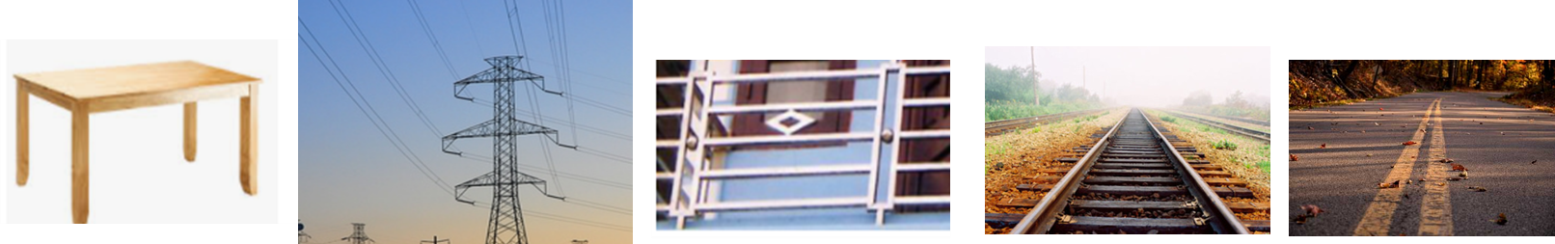
\includegraphics[width=0.75\linewidth]{image029}
			\end{center}
		\i Hình ảnh về 2 đường thẳng cắt nhau: Cái kéo, 2 mép tường, Tia laser, các con đường giao\linebreak thông, \ldots
		\begin{center}
%			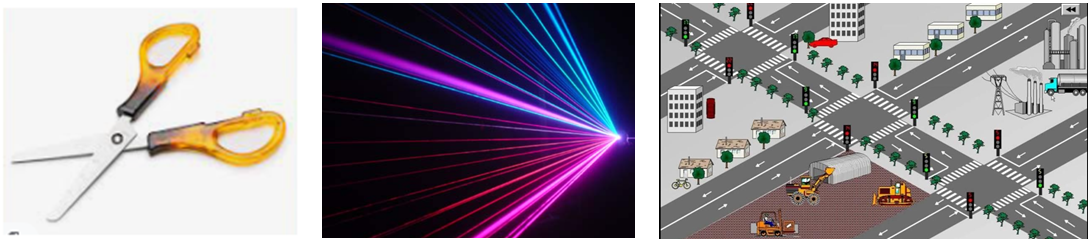
\includegraphics[width=0.75\linewidth]{image030}
		\end{center}
		\end{enumerate}
	
\end{Answer}
\begin{Answer}{4}
		\begin{enumerate}[a),leftmargin=*]
			\i Đường thẳng  $a$ đi qua $M$ và không đi qua $N$.
			\i Đường thẳng $b$ đi qua $Q$  và không đi qua $M$.
			\i Đường thẳng $c$ đi qua cả hai điểm $M,N$
		\end{enumerate}
	
\end{Answer}
\begin{Answer}{5}
	\begin{tabular}{p{0.5\textwidth} p{0.5\textwidth}}
		a)  & b) \\
		\begin{tikzpicture}
			\draw (0,0) -- (4,0) (0,1) -- (4, 1) (0,2) -- (4,2);
			\draw (4,0) node [right] {$c$};
			\draw (4,1) node [right] {$b$};
			\draw (4,2) node [right] {$a$};
		\end{tikzpicture}& \begin{tikzpicture}
		\draw (0.6,2.88)-- (-2.4,-0.12);
		\draw (0.4,-0.28)-- (-2.16,2.7);
		\draw (-2.92,1.28)-- (0.62,1.34);
		\draw[color=black] (0.4,2.41) node {$c$};
		\draw[color=black] (-1.72,2.73) node {$a$};
		\draw[color=black] (-2.62,1.17) node {$b$};
	\end{tikzpicture} \\
	 c) & d) \\
	 \begin{tikzpicture}
	\draw  (-4.,2.)-- (1.,2.);
	\draw  (-4.,1.)-- (1.,1.);
	\draw  (0.,3.)-- (-3.,0.);
	\draw[color=black] (0.16,1.87) node {$b$};
	\draw[color=black] (0.06,0.87) node {$a$};
	\draw[color=black] (-0.54,2.91) node {$c$};
	\draw [fill=uuuuuu] (-1.,2.) circle (2.0pt);
	\draw [fill=uuuuuu] (-2.,1.) circle (2.0pt);
\end{tikzpicture} & \begin{tikzpicture}
\draw (-0.2,2.64)-- (-2.56,0.08);
\draw (0.96,0.14)-- (-1.18,2.58);
\draw (-2.46,0.76)-- (1.08,0.82);
\draw[color=black] (0.04,1.65) node {$c$};
\draw[color=black] (-1.4,1.95) node {$a$};
\draw[color=black] (-0.78,0.59) node {$b$};
\end{tikzpicture}
	\end{tabular}
	
\end{Answer}
\begin{Answer}{6}
		\begin{tabular}{p{0.5\textwidth} p{0.5\textwidth}}
			a) & b) \\
			\begin{tikzpicture}
				\draw  (-4.,2.)-- (1.,2.);
				\draw  (-3.5,1.14)-- (0.56,2.88);
				\draw[color=black] (-2.76,1.23) node {$x$};
				\draw [fill=uuuuuu] (-1.4933333333333332,2.) circle (2.0pt);
				\draw[color=uuuuuu] (-1.36,2.33) node {$A$};
				\draw [fill=xdxdff] (-3.02,2.) circle (2.0pt);
				\draw[color=xdxdff] (-2.88,2.37) node {$M$};
				\draw [fill=xdxdff] (-0.08,2.) circle (2.0pt);
				\draw[color=xdxdff] (0.06,2.37) node {$N$};
				\draw [fill=xdxdff] (0.11344827586206918,2.6886206896551723) circle (2.0pt);
				\draw[color=xdxdff] (0.26,3.05) node {$P$};
			\end{tikzpicture}&
			\begin{tikzpicture}
				\draw  (-4.,2.)-- (1.,2.);
				\draw  (-2.32,1.)-- (1.74,2.74);
				\draw[color=black] (-1.58,1.09) node {$y$};
				\draw [fill=uuuuuu] (0.013333333333332476,2.) circle (2.0pt);
				\draw[color=uuuuuu] (0.16,2.33) node {$B$};
				\draw [fill=xdxdff] (-3.02,2.) circle (2.0pt);
				\draw[color=xdxdff] (-2.88,2.37) node {$M$};
				\draw [fill=xdxdff] (-1.34,2.) circle (2.0pt);
				\draw[color=xdxdff] (-1.2,2.37) node {$N$};
				\draw [fill=xdxdff] (1.2934482758620685,2.5486206896551726) circle (2.0pt);
				\draw[color=xdxdff] (1.44,2.91) node {$P$};
			\end{tikzpicture}\\
			\multicolumn{2}{l}{c)}\\
			\multicolumn{2}{l}{\begin{tikzpicture}
				\draw  (-4.,2.)-- (1.,2.);
				\draw  (-3.46,2.9)-- (-1.7,0.86);
				\draw [fill=xdxdff] (-0.88,2.) circle (2.0pt);
				\draw[color=xdxdff] (-0.74,2.37) node {$M$};
				\draw [fill=xdxdff] (0.38,2.) circle (2.0pt);
				\draw[color=xdxdff] (0.52,2.37) node {$N$};
				\draw[color=black] (-3.04,2.95) node {$z$};
				\draw [fill=uuuuuu] (-2.683529411764706,2.) circle (2.0pt);
				\draw[color=uuuuuu] (-2.54,2.33) node {$C$};
				\draw [fill=xdxdff] (-2.1179854529424738,1.344483138637867) circle (2.0pt);
				\draw[color=xdxdff] (-1.98,1.71) node {$P$};
			\end{tikzpicture}}
		\end{tabular}
	
\end{Answer}
\begin{Answer}{7}
		Bài 14. Có 6 đoạn thẳng có mút là 2 trong 4 điểm $A,B,C,D$:
		Đoạn thẳng $AB$, $AC$, $AD$, $BC$, $BD$, $CD$.
	
\end{Answer}
\begin{Answer}{8}
		\begin{enumerate}[a),leftmargin=*]
			\i Có tất cả 8 tia: $Ax,Ay,Bx,By,Cx,Cy,Dx,Dy$.
			\i Điểm $B$ nằm trên tia $Ax,Bx,By$.\\
			Tia đối của tia $Ay$ là tia $Ax$.\\
			Tia đối của tia $Ax$ là tia $Ay$.\\
			Tia đối của tia $Bx$ là tia $Bx$.\\
			Tia đối của tia $By$là tia $Bx$.\\
			\i Hai tia $AC$ và tia $CA$ không là hai tia đối nhau
		\end{enumerate}
	
\end{Answer}
\begin{Answer}{9}
		Ta có thể vẽ như sau:
		\begin{center}
			\begin{tikzpicture}
				\draw  (-1.92,4.04)-- (-3.78,1.88);
				\draw  (-3.78,1.88)-- (0.36,1.84);
				\draw  (0.36,1.84)-- (-1.92,4.04);
				\draw  (-3.78,1.88)-- (-0.8624928275422378,3.0195983423653177);
				\draw  (0.36,1.84)-- (-2.8289853788214443,2.9844040762073547);
				\draw  (-1.92,4.04)-- (-1.8201829510185985,1.861064569575059);
		
					\draw [fill=ududff] (-1.92,4.04) circle (2.0pt);
					\draw[color=ududff] (-1.78,4.41) node {$A$};
					\draw [fill=ududff] (-3.78,1.88) circle (2.0pt);
					\draw[color=ududff] (-4.14,1.77) node {$B$};
					\draw [fill=ududff] (0.36,1.84) circle (2.0pt);
					\draw[color=ududff] (0.66,1.91) node {$C$};
					\draw [fill=xdxdff] (-0.8624928275422378,3.0195983423653177) circle (2.0pt);
					\draw[color=xdxdff] (-0.62,3.41) node {$M$};
					\draw [fill=xdxdff] (-2.8289853788214443,2.9844040762073547) circle (2.0pt);
					\draw[color=xdxdff] (-3.26,3.29) node {$N$};
					\draw [fill=xdxdff] (-1.8201829510185985,1.861064569575059) circle (2.0pt);
					\draw[color=xdxdff] (-1.56,1.59) node {$P$};
					\draw [fill=uuuuuu] (-1.8510505349070308,2.6334609113144305) circle (2.0pt);
					\draw[color=uuuuuu] (-1.72,2.97) node {$G$};
		\end{tikzpicture}
		\end{center}
	
\end{Answer}
\begin{Answer}{10}
	Có 10 điểm là giao điểm của đúng 2 đường: $A,B,C,D,E,M,N,O,P,Q.$
	
\end{Answer}
\begin{Answer}{11}
		Do cứ 2 điểm thì tạo thành 1 đường thẳng và không có 3 điểm nào thẳng hàng nên 2022 điểm sẽ nối được với 2021 điểm và mỗi đường thẳng sẽ bị trùng nên ta có:
		
		Số đường thẳng được tạo thành là: $\dfrac{2022.2021}{2}=2043231$ (đường thẳng)
		
		Vậy tạo thành được 2043231 đường thẳng khác nhau có đầu mút là 2 trong 2022 điểm đã cho.
	
\end{Answer}
\begin{Answer}{12}
		Bài 19. Giả sử 1998 điểm phân biệt không có 3 điểm nào thẳng hàng, khi đó:
		
		Số đường thẳng được tạo thành là: $\dfrac{1998.(1998-1)}{2}=1995003$(đường thẳng)
		
		5 điểm thẳng hàng tạo thành 1 đường thẳng.
		
		5 điểm không thẳng hàng tạo thành $\dfrac{5.4}{2}=10$ (đường thẳng)
		
		Số đường thẳng bị giảm đi là: $10-1=9$ (đường thẳng)
		
		Vậy có tất cả: $1995003-9=1994994$ (đường thẳng)
	
\end{Answer}
\begin{Answer}{13}
		Bài 20. Do cứ 2 điểm thì tạo thành 1 đường thẳng và không có 3 đường thẳng nào đồng quy nên cứ mỗi đường thẳng sẽ giao với $n-1$ đường thẳng và tạo ra $n-1$ giao điểm
		
		Vậy với $n$ đường thẳng cắt nhau có số giao điểm là: $\dfrac{n(n-1)}{2}$ (do số giao điểm bị trùng)
		
		Theo đề ra: $\dfrac{n(n-1)}{2}=780 \Leftrightarrow n(n-1)=1560$
		
		Do $40\cdot39=1560$ nên $n=40$(đường thẳng).
	
\end{Answer}
\begin{Answer}{14}
		Bài 21. Giả sử 1015 đường cắt nhau trong đó không có 3 đường thẳng nào đồng quy. Khi đó số đường thẳng được tạo thành là:
		\begin{align*}
			\dfrac{1015\cdot1014}{2}=514605 \text{ (đường thẳng)}
		\end{align*}
		15 đường thẳng đồng quy thì có số giao điểm là 1.
		
		15 đường thẳng không đồng quy thì số giao điểm là:
		\begin{align*}
			\dfrac{15\cdot14}{2}=105 \text{ (đường thẳng)}
		\end{align*}
		Số giao điểm bị giảm là: $105-1=104$(đường thẳng)
		
		Vậy với 1015 đường thẳng cắt nhau trong đó có 15 đường đồng quy thì có số giao điểm là: $514605-104=514501$(đường thẳng)
	
\end{Answer}
\begin{Answer}{15}
		Mỗi một thành viên của đội Thái Bình Dương sẽ kết nối với 8 thành viên của đội Đại Tây Dương cần 8 đường dây.
		
		Vậy 5 thành viên của đội Đại Tây Dương kết nối với 8 thành viên của đội Đại Tây Dương cần: $5\cdot8=40$ (đường dây)
	
\end{Answer}
\begin{Answer}{16}
		\begin{tabular}{p{0.33\linewidth} p{0.33\linewidth} p{0.33\linewidth}}
			a) & b) &c)\\
			\begin{tikzpicture}
				\draw  (-1.52,3.34)-- (0.72,1.68);
				\draw  (-1.52,1.7)-- (0.84,3.28);
					\draw [fill=ududff] (-1.52,3.34) circle (2.0pt);
					\draw [fill=ududff] (0.72,1.68) circle (2.0pt);
					\draw [fill=ududff] (-1.52,1.7) circle (2.0pt);
					\draw [fill=ududff] (0.84,3.28) circle (2.0pt);
					\draw [fill=uuuuuu] (-0.3573436326574405,2.4783885849157814) circle (2.0pt);
			\end{tikzpicture}&
		\begin{tikzpicture}
			\draw  (-1.22,4.24)-- (-2.38,2.);
			\draw  (-2.38,2.)-- (1.14,2.02);
			\draw  (1.14,2.02)-- (-1.22,4.24);
			\draw  (-1.22,4.24)-- (-0.820277625334926,2.008862058946961);
			\draw  (-2.38,2.)-- (-0.18976490760144782,3.2708805486759385);
			\draw  (1.14,2.02)-- (-1.7957706814181542,3.128166960020116);
	
				\draw [fill=ududff] (-1.22,4.24) circle (2.0pt);
				\draw [fill=ududff] (-2.38,2.) circle (2.0pt);
				\draw [fill=ududff] (1.14,2.02) circle (2.0pt);
				\draw [fill=xdxdff] (-0.820277625334926,2.008862058946961) circle (2.0pt);
				\draw [fill=xdxdff] (-0.18976490760144782,3.2708805486759385) circle (2.0pt);
				\draw [fill=xdxdff] (-1.7957706814181542,3.128166960020116) circle (2.0pt);
				\draw [fill=uuuuuu] (-0.9657124187758623,2.8206381969906964) circle (2.0pt);
		\end{tikzpicture}&
	\begin{tikzpicture}[scale=0.6]
		\draw  (-4.,5.)-- (0.,5.);
		\draw  (0.,5.)-- (0.,1.);
		\draw  (0.,1.)-- (-4.,1.);
		\draw  (-4.,1.)-- (-4.,5.);
		\draw  (-2.,5.)-- (-2.,1.);
		\draw  (-4.,3.)-- (0.,3.);
		\draw  (-4.,5.)-- (0.,1.);
		\draw  (-4.,1.)-- (0.,5.);
			\draw [fill=ududff] (-4.,5.) circle (2.0pt);
			\draw [fill=ududff] (0.,5.) circle (2.0pt);
			\draw [fill=ududff] (0.,1.) circle (2.0pt);
			\draw [fill=ududff] (-4.,1.) circle (2.0pt);
			\draw [fill=xdxdff] (-2.,5.) circle (2.0pt);
			\draw [fill=xdxdff] (-2.,1.) circle (2.0pt);
			\draw [fill=xdxdff] (-4.,3.) circle (2.0pt);
			\draw [fill=xdxdff] (0.,3.) circle (2.0pt);
			\draw [fill=uuuuuu] (-2.,3.) circle (2.0pt);
	\end{tikzpicture}
		\end{tabular}
	
\end{Answer}

%	\begin{Answer}{17}
		\begin{tikzpicture}
			\draw (0,0) --(5,0);
			\filldraw[black] (0,0) circle[radius = 2pt] node [above] {$A$};
			\filldraw[black] (2.5,0) circle[radius = 2pt] node [above] {$I$};
			\filldraw[black] (5,0) circle[radius = 2pt] node [above] {$B$};
			
			\draw (1.25,0.2) node [above] {$2.5\, cm$};
			\draw (3.75,0.2) node [above] {$2.5\, cm$};
		\end{tikzpicture}
	
\end{Answer}
\begin{Answer}{18}
		\begin{tikzpicture}
			\draw (0,0) -- (3, 0) (0,1) -- (2.5, 1) -- (5,1) (0,2) -- (5,2) (0,2) -- (-5,2);
			\filldraw[black] (0,0) circle[radius = 2pt] node[above]{$A$};
			\filldraw[black] (3,0) circle[radius = 2pt] node[above]{$B$};
			\filldraw[black] (1.5,0) circle[radius = 2pt] node[above]{$I$};
			\filldraw[black] (0,1) circle[radius = 2pt] node[above]{$D$};
			\filldraw[black] (2.5,1) circle[radius = 2pt] node[above]{$E$};
			\filldraw[black] (5,1) circle[radius = 2pt] node[above]{$F$};
			\filldraw[black] (0,2) circle[radius = 2pt] node[above]{$G$};
			\filldraw[black] (5,2) circle[radius = 2pt] node[above]{$H$};
			\filldraw[black] (-5,2) circle[radius = 2pt] node[above]{$K$};
			
			\draw (0.75,0.1) node[above]{$1.5\,cm$};
			\draw (2.25,0.1) node[above]{$1.5\,cm$};
			\draw (1.25,1.1) node[above]{$2.5\,cm$};
			\draw (3.75,1.1) node[above]{$2.5\,cm$};
			\draw (2.5,2.1) node[above]{$5\,cm$};
			\draw (-2.5,2.1)node[above]{$5\,cm$};
		\end{tikzpicture}
	
\end{Answer}
\begin{Answer}{19}
		Vì  $C$ nằm giữa $A,B$ nên ta có: $AB=AC+BC$
		
		$\Rightarrow 5=AC+3\Rightarrow AC=5-3=2$ (cm)
		
		Vì $B$ nằm giữa $A,D$ nên $AD=AB+BD$
		
		$\Rightarrow AD=5+1=6$ (cm)
	
\end{Answer}
\begin{Answer}{20}
		\begin{enumerate}[a),leftmargin=*]
			\i	Vì $A$ nằm giữa $O,B$ nên $OB=OA+AB=5+9=14\left( cm \right)$
			\begin{center}
				\begin{tikzpicture}[scale=0.75]
					\draw[->] (0,0) -- (18,0);
					\filldraw[black] (0,0) circle[radius = 2pt] node [above] {$O$};
					\filldraw[black] (5,0) circle[radius = 2pt] node [above] {$A$};
					\filldraw[black] (14,0) circle[radius = 2pt] node [above] {$B$};
					\draw (18,0) node[above] {$x$};		
					\draw (2.5,0.1) node[above] {$5\,cm$};		
					\draw (7.5,0.1) node[above] {$9\,cm$};						
				\end{tikzpicture}
			\end{center}
			\i TH1: $M$ nằm giữa $A,N$\\
			Ta có: $AN=AM+MN=7+2=9$ (cm)
			\begin{center}
				\begin{tikzpicture}[scale=0.75]
					\draw[->] (0,0) -- (14,0);
					\filldraw[black] (0,0) circle[radius = 2pt] node [above] {$A$};
					\filldraw[black] (7,0) circle[radius = 2pt] node [above] {$M$};
					\filldraw[black] (9,0) circle[radius = 2pt] node [above] {$N$};
					\draw (14,0) node[above] {$x$};		
					\draw (3.5,0.1) node[above] {$7\,cm$};		
					\draw (8,0.1) node[above] {$2\,cm$};						
				\end{tikzpicture}
			\end{center}
			TH2: $N$ nằm giữa $A,M$\\
			Ta có: $AM=AN+NM$\\
			$\Rightarrow 7 = AN + 2$\\
			$\Rightarrow AN = 7 - 2 = 5$ (cm).
		\end{enumerate}
	
\end{Answer}
\begin{Answer}{21}
		Vì $M$ thuộc đoạn thẳng $AB$  nên ta có: $AB = MB + MA$\\
		$\Rightarrow 10 = MB + MA$\\
		Mà $MB - MA = 4$\\
		Khi đó $MB = 7$ cm; $MA = 3$ cm.
	
\end{Answer}
\begin{Answer}{22}
		Vì $P$ là trung điểm của $MI$ nên ta có: $MP = IP = \dfrac{MI}{2}$\\
		$\Rightarrow MI = 2IP = 2\cdot 3 = 6$ (cm)\\
		Vì $I$ là trung điểm của $MN$ nên ta có: $MI = IN = \dfrac{MN}{2}$\\
		$\Rightarrow MN = 2MI = 2\cdot 6 = 12$ (cm)\\
		Vậy $MN = 12$ (cm)
	
\end{Answer}
\begin{Answer}{23}
		\begin{enumerate}[a),leftmargin=*]
			\i Khi sử dụng thước đo độ dài:
			\begin{enumerate}[+,leftmargin=*]
				\i Đo độ dài của bàn học và ghi chú lại số liệu
				\i Điểm chính giữa của bàn học chính là trung điểm của đoạn thẳng đo được
				\i Dựa vào số liệu đã ghi chú và áp dụng công thức tính trung điểm đoạn thẳng xác định số đo
				\i Sử dụng số đo tính toán được áp dụng lên bàn học đó là điểm chính giữa của bàn
			\end{enumerate}
			\i Khi sử dụng đoạn dây vừa đủ:
			\begin{enumerate}[+,leftmargin=*]
				\i Điểm chính giữa của bàn học là trung điểm của đoạn dây chúng ta sử dụng
				\i Gấp đôi đoạn dây lại sao cho hai đầu dây bằng nhau, đánh dấu điểm chính giữa của đoạn dây
				\i Khi đó điểm đánh dấu chính là trung điểm của đoạn dây hay cũng là điểm chính giữa của bàn học
			\end{enumerate}
		\end{enumerate}
	
\end{Answer}
\begin{Answer}{24}
		Chọn điểm $A$  trùng với điểm thấp nhất của vòng quay mặt trời (so với mặt đất)
		
		Chọn điểm $B$  trùng với điểm cao nhất của vòng quay mặt trời (so với mặt đất)
		
		Khi đó, độ đài đoạn thẳng  $AB$ là: $AB = 64-8 = 56$ (cm)
		
		Theo cách xây dựng của vòng quay mặt trời thì điểm cao nhất của trục sẽ trùng với trung điểm của đoạn thẳng  $AB$, nên trung điểm của đoạn thẳng $AB$ nằm ở độ cao là: $\dfrac{AB}{2} = \dfrac{56}{2} = 28$ (m)
		Như vậy, trục của vòng quay mặt trời sẽ nằm ở độ cao $28 + 8 = 36$ (m)
	
\end{Answer}
\begin{Answer}{25}
		Vì $P$ là trung điểm của $ON$ nên ta có: $OP = PN = \dfrac{ON}{2} = \dfrac{6}{2} = 3$ (cm)
		
		Vì $O$ nằm giữa $M,P$ và $OM=OP=3cm$ nên $O$ là trung điểm của $MP$.
	
\end{Answer}
\begin{Answer}{26}
		Vì $M$ nằm giữa $A,B$ và $AM=MB=\dfrac{AB}{2}=\dfrac{a}{2}$ nên $M$ là trung điểm của đoạn thẳng$AB$
		\begin{center}
			\begin{tikzpicture}
				\draw (0,0) -- (8,0);
				\filldraw[black] (0,0) circle[radius = 2pt] node [above] {$A$};
				\filldraw[black] (3,0) circle[radius = 2pt] node [above] {$M$};
				\filldraw[black] (6,0) circle[radius = 2pt] node [above] {$B$};
				\draw (1.5,0.1) node[above] {$\dfrac{a}{2}$};	
			\end{tikzpicture}
		\end{center}
	
\end{Answer}
\begin{Answer}{27}
		TH1:
		\begin{center}
			\begin{tikzpicture}
				\draw (0,0) -- (9,0);
				\filldraw[black] (0,0) circle[radius = 2pt] node [above] {$A$};
				\filldraw[black] (3,0) circle[radius = 2pt] node [above] {$C$};
				\filldraw[black] (6,0) circle[radius = 2pt] node [above] {$D$};
				\filldraw[black] (9,0) circle[radius = 2pt] node [above] {$B$};
			\end{tikzpicture}
		\end{center}
		Vì $C$ nằm giữa $A,D$ nên ta có: $AC+CD=AD$\\
		Vì $D$ nằm giữa $B,C$ nên ta có: $BC+CD=BC$\\
		Mà $AC=BD$ và $CD$ chung $\Rightarrow AD=BC$\\
		TH2:
		\begin{center}
			\begin{tikzpicture}
				\draw (0,0) -- (9,0);
				\filldraw[black] (0,0) circle[radius = 2pt] node [above] {$A$};
				\filldraw[black] (3,0) circle[radius = 2pt] node [above] {$D$};
				\filldraw[black] (6,0) circle[radius = 2pt] node [above] {$C$};
				\filldraw[black] (9,0) circle[radius = 2pt] node [above] {$B$};
			\end{tikzpicture}
		\end{center}
		Vì $D$ nằm giữa $A,C$ nên ta có: $AC=AD+DC\Rightarrow AD=AC-DC$\\
		Vì $C$ nằm giữa $B,D$ nên ta có: $BD=BC+DC\Rightarrow BC=BD-DC$\\
		Mà $AC=BD$ và $DC$ chung $\Rightarrow AD=BC$
	
\end{Answer}
\begin{Answer}{28}
		Vì $A$ nằm giữa $O,B$ nên ta có: $OB=OA+AB=a+b$\\
		Vì $C$ là trung điểm của $OB$ nên ta có: $OC=CB=\dfrac{OB}{2}=\dfrac{a+b}{2}$\\
		Vì $A$ nằm giữa $O,C$ nên ta có: $OC=OA+AC$\\
		\begin{center}
			\begin{tikzpicture}
				\draw (0,0) -- (13,0);
				\filldraw[black] (0,0) circle[radius = 2pt] node [above] {$O$};
				\filldraw[black] (4,0) circle[radius = 2pt] node [above] {$A$};
				\filldraw[black] (5,0) circle[radius = 2pt] node [above] {$C$};
				\filldraw[black] (9,0) circle[radius = 2pt] node [above] {$B$};
				\draw (13,0.1) node[above] {$x$};
			\end{tikzpicture}
		\end{center}
		$\Rightarrow \dfrac{a + b}{2} = a + AC$\\
		$\Rightarrow AC = \dfrac{a+b}{2} - a = \dfrac{b-a}{2}$\\
		Vậy $AC = \dfrac{b-a}{2}$
	
\end{Answer}
\begin{Answer}{29}
		Vì $A$ nằm giữa $B,C$ và $3AB=4AC$ nên ta chia $BC$ thành 7 phần bằng nhau và xác định điểm $A$ như hình vẽ.
		\begin{center}
			\begin{tikzpicture}
				\draw (0,0) -- (14,0);
				\filldraw[black] (0,0) circle[radius = 2pt] node [above] {$B$};
				\filldraw[black] (2,0) circle[radius = 2pt];
				\filldraw[black] (4,0) circle[radius = 2pt] node [above] {$I$};
				\filldraw[black] (6,0) circle[radius = 2pt];
				\filldraw[black] (8,0) circle[radius = 2pt] node [above] {$A$};
				\filldraw[black] (10,0) circle[radius = 2pt];
				\filldraw[black] (12,0) circle[radius = 2pt];
				\filldraw[black] (14,0) circle[radius = 2pt] node [above] {$C$};
			\end{tikzpicture}
		\end{center}
		Vì $I$ là trung điểm của $AB$ nên ta có: $BI=AI=\dfrac{AB}{2}$\\
		$\Rightarrow AI=2BI=2\cdot4=8$ (cm)\\
		Lại có: $3AB=4AC\Rightarrow AC=\dfrac{3AB}{4}=\dfrac{3\cdot8}{4}=6$ (cm)\\
		Vì $A$ nằm giữa $B,C$ nên ta có: $BC=AB+AC=8+6=14$ (cm)\\
		Vậy $BC=14$ (cm)
	
\end{Answer}
\begin{Answer}{30}
		Vì ${{A}_{1}}$ là trung điểm của $AB$ nên ta có: $A{{A}_{1}}=AB.\dfrac{1}{2}$ (m)\\
		Vì ${{A}_{2}}$ là trung điểm của $A{{A}_{1}}$ nên ta có: $A{{A}_{2}}=\dfrac{A{{A}_{1}}}{2}=AB\cdot\dfrac{1}{2}\cdot\dfrac{1}{2}$ (m)\\
		Vì ${{A}_{3}}$ là trung điểm của $A{{A}_{2}}$ nên ta có: $A{{A}_{3}}=\dfrac{A{{A}_{2}}}{2}=\dfrac{A{{A}_{1}}}{2}\cdot\dfrac{1}{2}=AB\cdot\dfrac{1}{2}\cdot\dfrac{1}{2}\cdot\dfrac{1}{2}$ (m)\\
		Vì ${{A}_{4}}$ là trung điểm của $A{{A}_{3}}$ nên ta có: $A{{A}_{4}}=\dfrac{A{{A}_{3}}}{2}=\dfrac{A{{A}_{2}}}{2}\cdot\dfrac{1}{2}=\dfrac{A{{A}_{1}}}{2}\cdot\dfrac{1}{2}\cdot\dfrac{1}{2}=AB\cdot\dfrac{1}{2}\cdot\dfrac{1}{2}\cdot\dfrac{1}{2}\cdot\dfrac{1}{2}$ (m)\\
		Như vậy, khi ta lấy trung điểm ${{A}_{n}}$ của $AB$ thì $A{{A}_{n}}=AB\cdot{{ \left(\dfrac{1}{2} \right)}^{n}}$ (m)\\
		Vậy độ dài đoạn thẳng $A{{A}_{20}}=AB.{{\left(\dfrac{1}{2} \right)}^{n}}=1\cdot{{ \left(\dfrac{1}{2} \right)}^{20}}={{\left(\dfrac{1}{2} \right)}^{20}}$ (m)
	
\end{Answer}
\begin{Answer}{31}
		Do cứ 2 điểm thì tạo thành 1 đường thẳng và không có 3 điểm nào thẳng hàng nên 10 điểm sẽ nối được với 9 điểm và mỗi đường thẳng sẽ bị trùng nên ta có:
		
		Số đường thẳng được tạo thành là: $\dfrac{10 \cdot 9}{2}=45 $ (đường thẳng)
		
		Vậy tạo thành được 45 đường thẳng khác nhau có đầu mút là 2 trong 10 điểm đã cho.
	
\end{Answer}
\begin{Answer}{32}
		Do $5AB = 8BM \Rightarrow Bm = \dfrac{5AB}{8}$\\
		Mà $Bi = \dfrac{AB}{2}$\\
		$\Rightarrow Mi = BM - BI = \dfrac{5}{8}AB - \dfrac{1}{2}AB = \dfrac{1}{8} AB$.\\
		$\Rightarrow \dfrac{1}{8} AB = 2$ (cm)\\
		$\Rightarrow AB = 16$ (cm)
	
\end{Answer}
\begin{Answer}{33}
		Vì $OA<OB$ nên $A$ nằm giữa $O$ và $B$ $\Rightarrow AB=b-a$.\\
		Vì $C$ là trung điểm của $OB$ nên $OC=CB=\dfrac{b}{2}$\\
		TH1: Nếu $a<\dfrac{b}{2}$thì $OA<OC\Rightarrow OA+AC=OC\Rightarrow AC=OC-OA=\dfrac{b}{2}-a$\\
		TH2: Nếu $a>\dfrac{b}{2}$thì $OC<OA\Rightarrow OC+AC=OA\Rightarrow AC=OA-OC=a-\dfrac{b}{2}$
		\begin{center}
			\begin{tikzpicture}
				\draw (0,0) -- (10,0);
				\filldraw[black] (0,0) circle[radius = 2pt] node [above] {$O$};
				\filldraw[black] (3,0) circle[radius = 2pt] node [above] {$A$};
				\filldraw[black] (4,0) circle[radius = 2pt] node [above] {$C$};
				\filldraw[black] (8,0) circle[radius = 2pt] node [above] {$B$};
				\draw (2.5,0.1) node[above] {$a$};
				\draw (9,0.1) node[above] {$x$};
			\end{tikzpicture}
		\end{center}
	
\end{Answer}
\begin{Answer}{34}
		Ta xét các trường hợp sau:\\
		TH1: $O$ cùng phía với 2 điểm $A,B.$
		\begin{center}
			\begin{tikzpicture}
				\draw (0,0) -- (12,0);
				\filldraw[black] (1,0) circle[radius = 2pt] node [above] {$C$};
				\filldraw[black] (3,0) circle[radius = 2pt] node [above] {$O$};
				\filldraw[black] (6,0) circle[radius = 2pt] node [above] {$A$};
				\filldraw[black] (11,0) circle[radius = 2pt] node [above] {$B$};
				\draw (2.5,0.1) node[above] {$a$};
				\draw (0,0.1) node[above] {$x$};
				\draw (12,0.1) node[above] {$y$};
			\end{tikzpicture}
		\end{center}
		Do $OA=3cm$; $OB=8cm$  và $O$ cùng phía với 2 điểm $A,B$  nên $A$  nằm giữa $O$ và $B$.\\
		$\Rightarrow AB=OB-OA=8-3=5$ (cm).\\
		$A$  là trung điểm của $CB \Rightarrow C$ thuộc tia đối của tia $AB$  hay $A$  nằm giữa $C,B$ và $AC=AB=5$ (cm).\\
		$\Rightarrow AC>AO \Rightarrow O$  nằm giữa $A,C$.\\
		$\Rightarrow OC=AC-AO=5-3=2$ (cm).\\
		TH2: $O$  khác phía với 2 điểm $A,B$.\\
		\begin{center}
			\begin{tikzpicture}
				\draw (0,0) -- (12,0);
				\filldraw[black] (1,0) circle[radius = 2pt] node [above] {$C$};
				\filldraw[black] (9,0) circle[radius = 2pt] node [above] {$O$};
				\filldraw[black] (6,0) circle[radius = 2pt] node [above] {$A$};
				\filldraw[black] (11,0) circle[radius = 2pt] node [above] {$B$};
				\draw (2.5,0.1) node[above] {$a$};
				\draw (0,0.1) node[above] {$x$};
				\draw (12,0.1) node[above] {$y$};
			\end{tikzpicture}
		\end{center}
		Do $O$  khác phía với 2 điểm $A,B$  nên $O$  nằm giữa $A$  và $B$.\\
		$\Rightarrow AB=OA+OB=3+8=11$ (cm).\\
		$A$  là trung điểm của $CB \Rightarrow C$ thuộc tia đối của tia $AB$  hay $A$  nằm giữa $C,B$ và $AC=AB=11$ (cm).\\
		$\Rightarrow A$ nằm giữa $C,O$ $\Rightarrow OC=OA+AC=3+11=14$ (cm).
	
\end{Answer}

%	\begin{Answer}{35}
		\begin{enumerate}[a),leftmargin=*]
			\i Các góc trong hình vẽ:
			\begin{enumerate}[--,leftmargin=*]
				\i $\widehat{xOy}$: đỉnh $O$; cạnh $Ox,Oy$.
				\i $\widehat{yOz}$: đỉnh $O$; cạnh $Oy,Oz$.
				\i $\widehat{xOz}$: đỉnh $O$; cạnh $Ox,Oz$.
			\end{enumerate}
			\i Các điểm nằm trong góc $\widehat{xOy}:\,\,N,P$.
			\begin{enumerate}[--,leftmargin=*]
				\i Các điểm nằm ngoài góc $\widehat{xOy}:\,\,M,K$.
				\i Các điểm nằm trong góc $\widehat{yOz}:\,\,M$.
				\i Các điểm nằm ngoài góc $\widehat{yOz}:\,\,N,P,K$.
				\i Các điểm nằm trong góc $\widehat{xOz}:\,\,M,N,P$.
				\i Các điểm nằm ngoài góc $\widehat{xOz}:\,\,K$.
			\end{enumerate}
		\end{enumerate}
	
\end{Answer}
\begin{Answer}{36}
		Các góc có đỉnh $A:\,\,\widehat{BAH},\widehat{BAM},\widehat{BAC},\widehat{HAM},\widehat{HAC},\widehat{MAC}$.
		
		Các góc có đỉnh $M:\,\,\widehat{AMC},\widehat{AMH},\widehat{AMB}$.
		
		Các góc có đỉnh .
	
\end{Answer}
\begin{Answer}{37}
		\begin{enumerate}[a),leftmargin=*]
			\i Góc nhọn: $\widehat{MNP}$; góc tù: $\widehat{mDn}$; góc vuông: $\widehat{ABC},\widehat{xGk},\widehat{yOz}$; góc bẹt: $\widehat{FEQ}$.
			\i Dùng êke kiểm tra lại kết quả.
			\i Dùng thước đo góc: $\widehat{MNP}={{30}^\circ},\widehat{yOz}={{90}^\circ},\widehat{ABC}={{90}^\circ},\widehat{mDn}={{135}^\circ},\widehat{FEQ}={{180}^\circ},\widehat{xGk}={{90}^\circ}$
		\end{enumerate}
	
\end{Answer}
\begin{Answer}{38}
		Góc tạo bởi kim giờ và kim phút là:
		\begin{enumerate}[a),leftmargin=*]
			\i góc nhọn: lúc 2 giờ, 11 giờ.
			\i góc tù: lúc 4 giờ, 5 giờ.
			\i góc bẹt: lúc 6 giờ.
			\i góc vuông: lúc 3 giờ, 9 giờ.
		\end{enumerate}
	
\end{Answer}
\begin{Answer}{39}
		Hình ảnh thực tế về góc:
		\begin{enumerate}[+,leftmargin=*]
			\i Góc tạo bởi kim phút và kim giây của đồng hồ.
			\i Góc tạo bởi cái bóng và cây cột giữa trời nắng và mặt đất.
		\end{enumerate}
	
\end{Answer}
\begin{Answer}{40}
		\begin{enumerate}[a),leftmargin=*]
			\i Có 12 góc.
			\i $\widehat{ABC}={{55}^\circ};\widehat{BAC}={{80}^\circ};\widehat{ACB}={{45}^\circ};\widehat{ADB}={{110}^\circ};\widehat{BDC}={{130}^\circ};\widehat{ADC}={{120}^\circ}$
			$\widehat{CBD}={{25}^\circ},\widehat{DBA}={{20}^\circ},\widehat{BCD}={{20}^\circ},\widehat{DCA}={{25}^\circ},\widehat{BAD}={{40}^\circ},\widehat{CAD}={{40}^\circ}$
		\end{enumerate}
	
\end{Answer}
\begin{Answer}{41}
		\begin{enumerate}[a),leftmargin=*]
			\i Tam giác $ABC$ có:
			\begin{enumerate}[--,leftmargin=*]
				\i $\widehat{BAC}={{30}^\circ}$
				\i $\widehat{ABC}={{70}^\circ}$
				\i $\widehat{ACB}={{80}^\circ}$
				\i $\widehat{BAC}+\widehat{ABC}+\widehat{ACB}={{180}^\circ}$
			\end{enumerate}
			\i Tam giác đều $DEG$ có:
			\begin{enumerate}[--,leftmargin=*]
				\i $\widehat{D}={{60}^\circ}$
				\i $\widehat{G}={{60}^\circ}$
				\i $\widehat{E}={{60}^\circ}$
			\end{enumerate}
		\end{enumerate}
	
\end{Answer}
\begin{Answer}{42}
		Góc tạo bởi kim giờ và kim phút của đồng hồ:
		\begin{enumerate}[--,leftmargin=*]
			\i lúc 4 giờ: ${{120}^\circ}$
			\i lúc 9 giờ: ${{90}^\circ}$
			\i lúc 11 giờ: ${{30}^\circ}$
			\i lúc 6 giờ: ${{180}^\circ}$
		\end{enumerate}
	
\end{Answer}
\begin{Answer}{43}
		Những vạch số nằm trong góc tạo bởi
		\begin{enumerate}[a),leftmargin=*]
			\i kim giây và kim phút: 7; 6; 5; 4; 3
			\i kim giờ và kim phút: 11; 12; 1; 1
		\end{enumerate}
	
\end{Answer}
\begin{Answer}{44}
		\begin{enumerate}[a),leftmargin=*]
			\i Các góc có trong hình vẽ: $\widehat{mOz},\widehat{mOy},\widehat{mOx},\widehat{zOy},\widehat{zOx},\widehat{yOx}$
			\i Góc nhọn: $\widehat{mOz},\widehat{zOy},\widehat{yOx}$; góc vuông: $\widehat{mOn},\widehat{xOz}$; góc tù: $\widehat{xOm}$.
		\end{enumerate}
	
\end{Answer}
\begin{Answer}{45}
		A. Phòng bếp.
	
\end{Answer}
\begin{Answer}{46}
		Số góc tạo bởi hai trong năm tia là:
		\begin{enumerate}[--,leftmargin=*]
			\i Số góc tạo bởi tia $Ox$ với 1 trong 4 tia còn lại là: 4 góc.
			\i Số góc tạo bởi tia $Om$ với 1 trong 3 tia còn lại (không kể $Ox$) là: 3 góc.
			\i Số góc tạo bởi tia $Oy$ với 1 trong 2 tia còn lại (không kể $Ox,Oy$) là: 2 góc.
			\i Số góc tạo bởi tia $On$ với tia $Ot$ còn lại là: 1 góc.
		\end{enumerate}
		Vậy số góc tạo thành là: $4+3+2+1=10$ góc.
	
\end{Answer}
\begin{Answer}{47}
		Xét góc tạo bởi tia thứ nhất với 1 trong 3 tia còn lại có 3 góc.\\
		Xét góc tạo bởi tia thứ 2 với 1 trong 2 tia còn lại có 2 góc.\\
		Xét góc tạo bởi tia thứ 3 với 1 tia còn lại có 1 góc.\\
		Do đó, số góc tạo thành: $3+2+1=6$ góc.\\
		Vì $Oy,On$ là hai tia đối nên tạo thành 1 góc bẹt.\\
		Vậy số góc tạo bởi 2 trong 4 tia không kể góc bẹt là: $6-1=5$ góc.
	
\end{Answer}
\begin{Answer}{48}
		Số góc tạo bởi tia thứ nhất với 1 trong $n-1$ tia còn lại là $n-1$ góc.\\
		Số góc tạo bởi tia thứ hai với 1 trong $n-2$ tia còn lại là $n-2$ góc.\\
		\ldots \\
		Số góc tạo bởi tia thứ $n-1$ với tia thứ $n$ là 1 góc.\\
		Do đó, tổng số góc là: $1+2+...+n-2+n-1=n\cdot\left( n-1 \right):2$\\
		Ta có: $n\cdot\left( n-1 \right):2=21\Rightarrow n\cdot\left( n-1 \right)=42$\\
		mà $42=7\cdot6$ nên $n=7$
	
\end{Answer}
\begin{Answer}{49}
		Ta có:\\
		Xóa 1 tia gốc $O$ thì số góc giảm đi 10\\
		Khi chưa xóa tia, số góc tạo bởi tia đó với $n-1$ tia còn lại là $n-1$ góc.\\
		Số góc giảm đi 10 khi xóa 1 tia nên: $n-1=10 \Rightarrow n=11$.
	
\end{Answer}
\begin{Answer}{50}
		Ta có: $\widehat{MAN}$ là góc bẹt nên $\widehat{MAN}={{180}^\circ}$.\\
		$\widehat{MAT}+\widehat{NAT}=\widehat{MAN}\Rightarrow \widehat{MAT}+\widehat{NAT}={{180}^\circ}$\\
		mà  $\widehat{MAT}-\widehat{NAT}={{8}^\circ}$  nên:
		$\widehat{MAT}=\left({{180}^\circ}+{{8}^\circ}\right):2={{94}^\circ}$ \\
		$\widehat{NAT}=\left({{180}^\circ}-{{8}^\circ}\right):2={{86}^\circ}$ \\
	
\end{Answer}

%	\input{loigiaichuong31}
	\begin{Answer}{1}
		Gợi ý: Bác Sơn có thể đem tiền đến gửi ngân hàng để đồng tiền “sinh sôi”.
	
\end{Answer}
\begin{Answer}{2}
		Đáp số
		\begin{enumerate}[a),leftmargin=*]
			\i 124 triệu.
			\i Trước khi sang tháng thứ 51.
		\end{enumerate}
	
\end{Answer}
\begin{Answer}{3}
		Đáp số: 9336000 đồng.
	
\end{Answer}
\begin{Answer}{4}
		Hướng dẫn giải
		\begin{center}
			\begin{tabular}{|c|c|c|c|}
			\hline
			Tháng&Tiền gốc	&Tiền lãi&	Tiền phải trả\\
			\hline
			1&	5000000 đồng&	300000 đồng&	5300000 đồng\\
			\hline
			2&	5000000 đồng&	250000 đồng&	5250000 đồng\\
			\hline
			3&	5000000 đồng&	200000 đồng&	5200000 đồng\\
			\hline
			4&	5000000 đồng&	100000 đồng&	5100000 đồng\\
			\hline
			6&	5000000 đồng&	50000 đồng&	5050000 đồng\\
			\hline
		\end{tabular}
		\end{center}
	
\end{Answer}

	\begin{Answer}{5}
		Có thể có những khả năng sau đây
		\begin{enumerate}[--,leftmargin=*]
			\i Hoa làm rơi tiền.
			\i Hoa sử dụng tiền không có kế hoạch, nhầm lẫn…
			\i Hoa chi phí cho việc bán hàng quá nhiều. Lợi nhuận Hoa có là 800.000 đồng mới chỉ là lợi nhuận gộp chưa tính các chi phí như tiền điện thoại, tiền cước vận chuyển, tiền chi hoa hồng cho bạn bè giới thiệu (nếu có)
		\end{enumerate}
	
\end{Answer}
\begin{Answer}{6}
		\begin{enumerate}[a),leftmargin=*]
			\i 2000 cuốn/tháng.
			\i 2800 cuốn/tháng
		\end{enumerate}
	
\end{Answer}
\begin{Answer}{7}
		\begin{enumerate}[a),leftmargin=*]
			\i 70 sản phẩm và 420000 đồng
			\i 240 sản phẩm.
		\end{enumerate}
	
\end{Answer}

\end{document}